\PassOptionsToPackage{table}{xcolor}
\documentclass[12pt,onesided]{amsart} 
\usepackage{natbib}
\usepackage{amsmath}
\usepackage{pifont}
\usepackage[multiple]{footmisc}
\usepackage{subfigure}
\usepackage[T1]{fontenc}
\usepackage{xcolor}
\usepackage{multirow,multicol}
\usepackage{caption}
\usepackage{booktabs}
\usepackage{color}
\usepackage{setspace}
\usepackage{colortbl}
\usepackage{changebar}
\usepackage{dcolumn}
\usepackage{graphicx}
\usepackage{tikz}
\usepackage[section]{placeins}
\setkeys{Gin}{width=\linewidth,totalheight=\textheight,keepaspectratio}
\graphicspath{{graphics/}{../graphics/}}

\usepackage{hyperref}

\usepackage{geometry}
\geometry{verbose,tmargin=1in,bmargin=1in,lmargin=1in,rmargin=1in}


\doublespace

\usepackage{booktabs}
\usepackage{units}
\usepackage{fancyvrb}
\fvset{fontsize=\normalsize}
\usepackage{lipsum}

\usepackage{footnote}
\usepackage{url}
\usepackage[nolists,tablesfirst]{endfloat}
\usepackage{nameref}

\begin{document}

%\maketitle
\thispagestyle{empty}

{\sc \large \hskip .7cm The Reputational Impact of Investor-State Disputes}

% \begin{quote}
% \noindent Abstract. To what extent do alleged violations of international commitments damage state reputation? This paper explores this question with specific reference to investor-state disputes arising under the protection of  international investment agreements. Existing theory assumes that institutionalization of international commitments  raises the ex post costs of defection, including reputational damage, thereby creating strong incentives for state compliance. Our analysis significantly modifies this expectation by suggesting that the strength of the incentives for compliance vary with the breadth, visibility, and legitimacy of the monitoring, sanctioning, and enforcement mechanisms brought into play by particular sets of international institutions. Drawing on a replication of prior research linking investor-state disputes with reduced FDI as well as an original analysis of their impact on investment reputation, we find that the costs of state involvement in investment  dispute arbitration  are limited with respect to investment reputation and completely inconsequential for FDI flows. These findings have significant implications for the broader body of literature on international institutions.  \end{quote}
 
\setcounter{page}{1}

\section*{Introduction}

Research on the compliance of states with international commitments emphasizes the deterrent effect of reputational damage. The underlying assumption is that reneging on a formal commitment damages a state's reputation and jeopardizes future opportunities for international cooperation. Agreements that institutionalize state commitments are consequently expected to constrain state actors from engaging in uncooperative behavior as well as to induce other sets of actors to monitor and punish defections. The idea has gained particular traction in the study of international economic instruments, including debt contracts, investment treaties, and free trade agreements,\footnote{See, for example, \citet{simmons:2000}; \citet{tomz:2007}; \citet{buthe:milner:2014}; \citet{buthe:milner:2008}; \citet{allee:peinhardt:2011}; \citet{elkins:etal:2006}.} but it has also been applied to a broader range of international issues.\footnote{See, for example, \citet{fearon:1997} and \citet{simmons:danner:2010}.}

Somewhat surprisingly, however, the argument linking reputational concerns to compliance with formal agreements remains largely unexamined. Reputational damage has been inferred from evidence of shifting patterns of foreign lending or investment flows.\footnote{See \citet{tomz:2007} and \citet{allee:peinhardt:2011}.} Reputational indicators have also been utilized to explain state entry into formal international agreements as well as defection from them.\footnote{For recent explananations of treaty formation see \citet{elkins:etal:2006} and \citet{simmons:danner:2010}, and for defection \citet{allee:peinhardt:2011} and \citet{freeman:2013}.}  But prior research has not systematically explored the consequences of reneging on commitments for state reputation. This paper fills this gap by exploring the reputational impact of investor-state disputes arising under the protection of bilateral investment treaties (BITs) and other international investment agreements (IIAs).

Investment treaties, which are designed to attract foreign direct investment (FDI) by offering credible property rights protection to private sector actors, have become an increasingly important part of the international legal architecture. As of the end of 2012, 200 states had signed one or more of these agreements, with the total IIA universe approaching 4,000, including 2,857 BITS and 339 other agreements with investment provisions.\footnote{\citet{unctad:2013}} In most cases these IIAs not only formalize commitments to treat foreign investors fairly and equitably, but also include provisions giving investors the right to take investor-state disputes to international arbitration, out of range of the host country's legal system. According to a recent survey, 93 percent of BITs include such provisions, which are intended to guarantee investors that their claims will be adjudicated in an independent, impartial, and timely manner.\footnote{\citet{gaukordger:gordon:2012}: 8} Over the past two decades these provisions have led to a significant proliferation of investor-state dispute settlement (ISDS) cases.

As of the end of 2013, the United Nations Conference on Trade and Development (UNCTAD) had identified 514 treaty-based arbitrations of investor-state disputes involving 98 different nations;\footnote{\citet{unctad:2014}: 1} however, as arbitration often proceeds confidentially, the accuracy of the UNCTAD data is open to question and cannot be fully verified on the basis of other sources. What is known is that the predominant player in international investor-state disputes is the International Centre for the Settlement of International Disputes (ICSID), which is formally affiliated with the World Bank. The ICSID maintains public records of all of the international investment conflicts brought to it for resolution, the number of which totaled 459 as of December 31, 2013.\footnote{\citet{icsid:2014}: 7-8} Drawing on this database as well as data collected by UNCTAD, we create an original database to analyze how alleged treaty violations affect the reputation of states with the international investment community. 

In contrast to the theoretical claims developed in prior research, we show that the reputational impact of alleged investment treaty violations have for many years years been minimal. Clouding the effectiveness of disputes in altering perceptions were central characteristics of the ISDS process, particularly its narrow, decentralized, and untransparent monitoring and enforcement mechanisms, which provide international investors with little to no information with which to update their perceptions of investment risk in a particular country. Despite the public records maintained by ICSID, it is only in recent years that media outlets have started reporting on the cases brought to this arbitration tribunal. For many decades since the establishment of ICSID in 1965, the work being done there has gone unreported by the broader media. In recent years, this has very much changed, for example, 200 articles referencing ICSID cases have come out per year in the last three years. The extant literature has simply assumed that adverse reputational effects inevitably manifest from being brought in front of arbitration tribunals like the ICSID. Our empirical analyses show that the reputational impact of disputes has been nil for many years, and it is only recently as publicity around ICSID cases has grown that we find substantive changes in reputation from disputes.

The first part of the paper offers a brief overview of investor-state dispute settlement (ISDS) with central emphasis on the ICSID. The second section summarizes the basic argument regarding the importance of reputational concerns for sustaining international cooperation and outlines its central limitations, which revolve around its vagueness with respect to the causal linkages between defection from international commitments and state reputation. In the third section we attempt to replicate prior research indicating that involvement in investor-state dispute arbitration reduces FDI inflows and demonstrate that the evidence is singularly uncompelling. The fourth section turns to a more direct method of assessing the consequences of investment disputes and outlines our central research hypotheses, research design, data, and statistical methodology. The subsequent section draws upon two different types of models to explore the reputational costs of investment disputes. We conclude by comparing and contrasting the findings of the analysis with existing understandings of the efficacy of ``credible commitments'' and their significance for a state's reputation with the international investment community.

\section*{The Investor-State Dispute Settlement Process}

As indicated above, the dominant player in the international investor-state dispute settlement process is the ICSID, which was established as an autonomous international institution under a multilateral treaty drawn up by the executive directors of the World Bank in 1965. As of late 2013, a total of 158 states had ratified the ICSID Convention, not counting Bolivia, Ecuador, and Venezuela, which withdrew from membership between 2007 and 2012.\footnote{\citet{icsid:2014b}}  Prior to December 2013, other notable non-members include Brazil, Canada, India, Iran, Iraq, Poland, and South Africa, although several of these nations have agreed to arbitration under the ICSID's Affiliated Facility (AF), which is open to dispute arbitration and conciliation if one of the parties is a citizen of a member state. As of December 2013, 43 of the total of 459 investor-state disputes brought to the ICSID were arbitrated under the AF rules.\footnote{Ibid: 8}

The central purpose of the ICSID is to facilitate international flows of private investment by removing non-commercial risks and providing investors with access to impartial and flexible dispute settlement procedures. Under Article 25 of the ICSID Convention, the jurisdiction of the center extends to any legal dispute arising directly out of an investment between a contracting state and a national of another contracting state, providing the parties to the dispute consent in writing to ICSID arbitration. Once the parties accede to ICSID jurisdiction, neither can unilaterally withdraw nor refuse to enforce the ICSID arbitral award. Under Article 43, arbitration can only be discontinued if the parties agree to a settlement or dispute withdrawal, which has occurred in 36 percent of all ICSID disputes.\footnote{\citet{icsid:2014}: 13} Parties to investment disputes have the right to appeal for an annulment of arbitral settlements within the ICSID framework, although annulment is extremely unusual. Of the 180 awards rendered by the ICSID as of the end of 2013, only 13 resulted in a partial or full award annulment.\footnote{Ibid: 17}

The bases of consent that are invoked to establish ICSID jurisdiction in an investor-state dispute vary widely. BITs, which have been cited in 63 percent of ICSID arbitral claims, represent the single most important source, followed by investment contracts between states and foreign investors (19 percent), host state investment law (8 percent), free trade agreements (4.5 percent), and multi-lateral investment agreements (5.5 percent).\footnote{Ibid: 10} The ICSID also offers administrative assistance to arbitrations conducted under the rules of the United Nations Commission on International Trade Law (UNCITRAL) as well as to other venues for arbitral settlement, including the International Chamber of Commerce, the London Court of International Arbitration, the Permanent Court of Arbitration, the Cairo Regional Centre for International Commercial Arbitration, and the Arbitration Institute of the Stockholm Chamber of Commerce.

During its first two decades of existence, the ICSID played a relatively limited role, but that situation began to change with the expansion of foreign direct investment and bilateral investment treaties in the 1990s. Reliable information on arbitrations conducted outside the ICSID framework is limited, but according to UNCTAD's list of 390 disputes for the 1987-2010 period, 245 were arbitrated by the ICSID, 109 by ad hoc panels under the UNCITRAL arbitral rules, and the remainder by the International Chamber of Commerce or other venues.\footnote{\citet{unctad:2011}: 2} These data almost certainly understate the number of disputes that have been internationally arbitrated as well as the role of the ICSID. A case-by-case analysis indicates that the UNCTAD database misses 18 ICSID cases for the 1987-2010 period. UNCTAD records for the 2010 and 2011 also point to the growing importance of the ICSID, which was involved in 74.7 percent of all investment disputes in those two years.\footnote{See \citet{unctad:2011}: 1-2 and \citet{unctad:2012}: 1.}

The significance of the ICSID, however, cannot be defined merely in terms of the number of cases that have come under its jurisdiction. Also of importance are its visibility as an institution formally affiliated with the World Bank and the scope of its legal authority. Under the ICSID Convention, awards are binding on the parties to a dispute and enforceable as if they were final awards of national courts, with the ICSID's narrowly delimited annulment rules establishing the only avenue of appeal. Awards can thus be enforced in any country that adheres to the ICSID Convention. Moreover, unlike other international arbitration bodies, the ICSID maintains a public record of arbitral claims, making allegations about a host government's alleged violation of treaty commitments widely available to the international investment community. Arbitration in alternative venues is unlikely to have similar consequences, especially if the parties to the dispute remain anonymous and the outcome confidential, which appears to be the case with a significant number of investment disputes. For this reason, investor-state dispute arbitration within the ICSID framework is often assumed to carry high reputational costs, creating incentives for states to capitulate to foreign investor demands.\footnote{\citet{trakman:2013}: 619}  We explore this claim below, drawing upon data both for the ICSID as well as other ISDS venues.

\section*{The Political Economy of State Reputation}

Prior research in political economy has highlighted the importance of reputation for understanding the willingness of governments to comply with their international agreements. In Tomz's influential formulation, reputation establishes the basis for cooperation in a world of uncertainty, shifting preferences, and international anarchy.\footnote{\citet{tomz:2007}} Governments honor their debts and private investors lend money to foreigners because of reputational concerns -- not sanctions. Focusing on commitment and compliance in international monetary affairs, Simmons develops a similar line of argument: ``The acceptance of treaty obligations raises expectations about behavior that, once made, are reputationally costly for governments to violate.''\footnote{\citet{simmons:2000}: 819} \citeauthor{buthe:milner:2008} cite reputational effects to argue that international trade agreements provide mechanisms for making credible commitments to foreign investors: ``Violating an institutionalized commitment -- or not making amends to correct a violation that has occurred -- damages a country's reputation for keeping commitments, making future cooperation on the same and other issues more difficult and maybe impossible to achieve.''\footnote{\citet{buthe:milner:2008}: 746}  \citeauthor{buthe:milner:2009} and \citeauthor{elkins:etal:2006} utilize the same logic to explain why bilateral investment treaties represent credible commitments to foreign investors.\footnote{See \citet{buthe:milner:2009} and \citet{elkins:etal:2006}.}

The existing literature thus suggests that by raising ex post reputational costs, formal international commitments create incentives for state compliance. The implication is that high levels of compliance with international agreements are indicative of high reputational costs, whereas low levels of compliance are likely to be observed where reputational costs are low. Arguments emphasizing the importance of reputation also run from compliance to government reputation as illustrated by Allee and Peinhart's analysis of the impact of investor-state disputes.\footnote{\citet{allee:peinhardt:2011}} Similarly, in his study of the interwar period, Tomz finds that ``lemons'' who signaled a low regard for foreign commitments lost access to international credit markets.\footnote{\citet{tomz:2007}: 86-94} Thus not only are potential reputational costs assumed to cause compliance with international commitments; real reputational damage is the expected consequence of defection from those commitments. Logically the latter is the key causal issue. If compliance failures do not affect reputation, then reputational concerns are unlikely to yield much in the way of compliance.

For this reason, the subsequent analysis concentrates on exploring the direct reputational impact of alleged compliance failures. Prior research has largely sidestepped this issue, analyzing instead outcomes, such as FDI flows, that are presumed, but never actually shown, to be linked with reputation. In contrast, we explicitly test the causal impact of alleged defections from formal international commitments on reputation. In order to do so we disaggregate the concept of reputation and focus on compliance with a specific category of international agreements -- international investment treaties. As suggested by \citeauthor{brewster:2009}, existing theoretical accounts of the importance of reputation err on the side of vagueness, ignoring a number of obvious questions.\footnote{\citet{brewster:2009}} How do we define and measure reputation? Whose reputation matters, with whom, and reputation for what? A negative reputation for compliance with agreements on human rights or the environment can obviously coexist with a positive reputation for complying with loan contracts. Likewise, reputations within particular issue domains are of varying importance to different audiences. The international human rights community may attempt to bring a government's behavior into compliance with international norms by ``shaming and blaming'', but its activities are unlikely to affect that government's observance of the rules of the World Trade Organization. The mechanisms through which the monitoring, enforcement, and sanctioning of international commitments occurs also vary widely across international institutions and issue domains,\footnote{\citet{gaukordger:gordon:2012}} presumably making some types of commitments more costly to break than others. By focusing specifically on a government's reputation for protecting international investors, we can minimize these difficulties and open the door to more effective theorizing about role of reputation in international politics.

Our central point of theoretical departure is the established literature on investment treaties, which creates the expectation that allegations of a government's failure to comply with its commitments generate reputational costs, regardless of the findings of arbitral tribunals. According to \citeauthor{schwenzer:hachem:2011}, for example, ``the reputation of a State may be damaged by wrongfully initiated investment treaty arbitration against the State. Such harm to reputation may have quite severe financial consequences for the entire economy of the State concerned.''\footnote{\citet{schwenzer:hachem:2011}: 426} Likewise, in their research on the ICSID, \citeauthor{allee:peinhardt:2011} claim that, ``The filing of a case before ICSID immediately brands the respondent country as an actor that is hostile to investors''\footnote{\citet{allee:peinhardt:2011}: 414} and leads to ``substantial losses in FDI.''\footnote{Ibid: 429} A recent analysis of investment arbitration, likewise argues that ``when an investor commences an ICSID arbitration against a respondent state and the investor ultimately loses, the state may have a credible argument that its `investment reputation' has been unfairly tarnished.''\footnote{\citet{parish2011awarding}: 236} State actors share this view as evidenced by Turkey's request in Europe Cement \& Trade S.A. v. Turkey for ``an award of monetary compensation for the moral damage it has suffered to its reputation and international standing through the bringing of a claim that is baseless and founded on fabricated documents.''\footnote{Europe Cement Investment \& Trade S.A. v. Republic of Turkey. 2009. ICSID Case No. ARB(AF)/07/02: 177} 

While these arguments are intrinsically plausible, three related characteristics of the prevailing international investment regime attenuate the potential significance of alleged investment treaty violations for state reputation. First, unlike the WTO, where governments press complaints before an international forum, the current ISDS process externalizes monitoring costs to individual private firms and sanctioning to ad hoc arbitral panels. Arbitral deliberations are also constrained to the facts of an individual case and do not necessarily establish legal precedents for other investment disputes. For this reason investor-state dispute arbitration has not only produced inconsistent results,\footnote{\citet{franck:2005}} but even opposing ones in parallel cases involving identical sets of facts and parties but different treaties and arbitral tribunals.\footnote{For example, see \citet{franck:2005}; \citet{kim2011annulment}; \citet{egli2006don}. For an example of a specific case compare the rulings issued in CME Czech Republic B.V. v Czech Republic and Lauder v Czech Republic: ``Final Award in the Matter of an UNCITRAL Arbitration'' 2001; ``UNCITRAL Arbitration Proceedings CME Czech Republic B.V. (The Netherlands) vs. The Czech: Final Award'' 2003.} The outcome of investor-state dispute arbitration is therefore rather uncertain and the meaning and significance of arbitral awards, whether positive, negative, or inconclusive with respect to a government charged with treaty violations, limited to the specifics of a particular dispute. Further given the relative narrowness of the current ISDS regime the assumption that alleged investment treaty violations generate significant reputational costs is implausible, particularly since reputations are presumably not only rather sticky but also constructed around multiple and widely varied types of observations. A state's alleged failure to comply with a particular investment treaty in its dealing with a single private firm is therefore unlikely to entail significant reputational costs.

Compounding this limitation is a second characteristic of investment dispute settlement procedures: namely, information about an investment dispute may remain too limited to allow the investment community to gauge the extent to which treaty violations have occurred, especially for cases arbitrated confidentially. In its dispute database, for example, \citeauthor{unctad:2010} includes cases described in such terms as ``an investor-State dispute under a BIT between a European investor and an African nation.''\footnote{\citet{unctad:2010}} But even for claims involving the relatively public ICSID arbitration process, information regarding the specifics of a case may remain restricted if both parties do not consent to the publication of the award rendered by an arbitral tribunal.\footnote{Amendments to the ICSID's arbitration rules in 2006, however, mandate the Centre to publish excerpts of the legal reasoning applied by arbitration tribunals in reaching their decisions in specific cases \citep{antonietti:2006}. UNCITRAL has also adopted new rules on transparency effective 1 April 2014, but they only apply to treaties concluded prior to that date at the agreement of the disputing parties. For UNCITRAL disputes brought under treaties concluded at a subsequent date, exceptions to the new rules require the agreement of both disputing parties (\citealp{uncitral:2013}: 33-40).}  To add to the lack of transparency, a high albeit unknown proportion of cases are settled or discontinued before they are formally arbitrated, preventing the facts of a dispute from being publically disclosed. 

Reputational costs are further muted by the relative lack of finality that characterizes investor-state dispute proceedings, which are open to further avenues of appeal, except within the ICSID framework, in which the only way to reverse a ruling is via the annulment process. But even annulments are not final, as plaintiffs can file for resubmission. Hence some cases, such as Enron Creditors Recovery Corporation and Ponderosa Assets, L.P. v Argentine Republic,\footnote{ICSID Case No. ARB/01/3} which was originally registered in 2001, ``lost'' or ``decided'' in 2007, annulled in 2010, resubmitted the same year, and still pending as of mid-2014, may convey uncertain and less than timely information to the investment community, magnifying the effect of limited transparency. 

The third limitation on reputational impact is the contested legitimacy of the current ISDS regime. Particularly, controversial are the limitations it imposes on the power of the state to regulate in the public interest, which often bring treaty obligations into collision with other sets of international norms, including democratic decision-making, human rights, global health, and environmental protection, reducing the reputational impact of disputes. Regardless of their final resolution, for example, it is hard to imagine that disputes involving state regulation of tobacco use, such as Philip Morris v. Uruguay or Philip Morris v. Australia actually create serious doubts about a country's commitment to treat investors fairly or damage reputations with the international investment community.\footnote{See ICSID ARB/10/7 and PCA Case No. 2012-12, respectively.} 

The failure of states to comply with arbitral decisions, which presumably carries much higher reputational costs than allegations of treaty non-compliance, is a symptom of this legitimacy problem. Even though Article 54 of the ICSID Convention establishes particularly strong legal obligations with respect to compliance with arbitral rulings, a number of states have refused to honor ICSID awards, including Kazakhstan, Ecuador, Congo, Russia, and Bolivia. The record in this regard is held by Argentina, which has been challenged before the ICSID more times than any other nation and has yet to comply fully with a single adverse ruling. Uncompensated investors, including CMS Gas Transmission Company, which was awarded \$132 million by an ICSID tribunal in 2005, have transferred their awards at undisclosed sums to banking subsidiaries specializing in distressed debts.\footnote{\citet{peterson:2009}} Even after the U.S. brought diplomatic pressures to bear on the country, including the suspension of U.S. trade preferences and a veto of lending by the World Bank and Inter-American Development Bank, the Argentine government only agreed to a settlement of its obligations to five companies, and this settlement involved a 25 percent discount of the original awards with payment to be rendered in Argentine bonds.\footnote{\citet{nacion:2013}} 

Given the relatively narrow, specific, decentralized, opaque, and potentially ineffective  monitoring, santioning, and enforcement mechanisms created by the ISDS regime, as well as its contested legitimacy, the presumption that the registration of an investor-state dispute carries significant reputational costs with the international investment community warrants further investigation. Investment disputes between states and individual firms, especially disputes settled prior to arbitration, adjudicated under a veil of confidentiality, open to further appeals or petitions for annulment, or involving conflicting norms regarding state sovereignty, convey only limited and ambiguous information about government behavior. Likewise, the sanctioning and enforcement mechanisms brought into play by disputes emerging under treaties are too specific, prolonged, and uncertain to allow investors to update their perceptions of investment risk with any degree of confidence. For these reasons, we depart from the conventional wisdom about the reputational costs of investor-state dispute involvement.

\section*{Replication of Prior Research}

We begin our analysis of the consequences of alleged investment treaty violations by revisiting the empirical analysis of \citeauthor{allee:peinhardt:2011}, which examines the impact of ICSID dispute involvement on foreign investment flows. Their research findings suggest that BITs increase FDI flows into countries that sign them, but only if those countries do not subsequently become involved in investor-state dispute arbitration at the ICSID.\footnote{\citet{allee:peinhardt:2011}} Allee and Peinhardt's work on this subject marked the first empirical examination of how ICSID disputes could adversely affect FDI flows, and their 2011 analysis has been cited extensively.\footnote{For example, see \citet{berger2011more}; \citet{poulsen2013claim}; \citet{wellhausen2013}; \citet{haftel2013delayed}; \citet{kerner2014}.} Their key finding is that countries experience significant losses of FDI by becoming a respondent in an ICSID arbitral claim and suffer even greater losses if they lose an ICSID dispute. Since these findings pose an important challenge to our central line of theoretical argument, we begin our analysis by replicating their study. In the process of doing so, we highlight a severe methodological problem in their empirical strategy.

For their dependent variable, Allee and Peinhardt use net FDI inflows less FDI outflows. They correctly highlight the importance of choosing this dependent variable as it best enables them to test how their reputational argument should apply to both current and potential investors. Specifically, they note that, ``firms who currently have investment in a country are likely to reconsider the investment climate in the host country \ldots on an ongoing basis'' and ``potential new investors are likely to reconsider whether a potential host country \ldots has been a defendant in ICSID disputes.''\footnote{\citet[p. 419--420]{allee:peinhardt:2011}} Thus for observations that have higher outflows than inflows their net FDI variable would be negative. Accounting for both positive and negative values introduces important variation, which their theoretical framework would argue can be explained by countries facing a higher number of ICSID disputes. 

The problem arises in their attempt to address the skewness of the net FDI variable through taking the log. In doing so, Allee and Peinhardt disregard the fact that logarithms of zero and negative numbers are not defined and therefore registered as missing in most statistical programs. They make no attempt to address this problem and, as a result, mistakenly exclude a notable number of country-year observations with negative or zero flows. Given their argument about the adverse reputational ramifications of ICSID disputes involvement on FDI flows, one could argue that the observations with negative flows are the most relevant portion of their dataset. In our replication of their analysis, we correct for this error by following the simple procedure suggested by \citeauthor{li:2009}, which calls for adding a constant so that each value is greater than zero before logging.\footnote{\citet{li:2009}} 

The impact of Allee and Peinhardt's error is readily apparent in Table \ref{tab:allee}. In the first column of the table, we exactly replicate their results for their base model that assesses the impact of pending ICSID disputes over the 1984-2007 period. In column two, we follow the exact same procedure except we log FDI flows in the correct way. Comparing the results of columns 1 and 2, it becomes evident that after including zero and negative FDI observations, ICSID dispute involvement does not significantly affect FDI flows. The results presented in other columns of the table are consistent with this finding. Column three shows the results from Allee and Peinhardt's model on the effect of disputes filed in the past two years, and column five uses disputes filed in the past five years. Columns four and six again show the results after correctly logging FDI flows, an in each case we see that Allee and Peinhardt's original findings do not hold. For reasons of space, we do not report our findings with respect to other sets of Allee and Peinhardt's results, which address the impact of ICSID disputes lost or settled over the past two and five years as as well as the impact of disputes lost over the past two years controlling for pending disputes. The results for these additional estimations, however, follow the same pattern as those reported in Table \ref{tab:allee}. We simply find no evidence that foreign investment flows are responsive to ICSID activity.\footnote{Estimations utilizing unlogged FDI are very similar.} Given the nature of these findings, we turn to a more direct test of the proposition that becoming a respondent in an ICSID dispute carries significant reputational costs.

% \newpage

\begin{table}[ht]
\vspace{1cm}
\centering
{\footnotesize
\caption{The Impact of ICSID Arbitration on FDI Inflows}
\label{tab:allee}
\begin{tabular}{lr@{} lr@{}lr@{}lr@{}lr@{}lr@{}lr@{} }
	\hline\hline
	~ & \multicolumn{4}{c}{(1)} & \multicolumn{4}{c}{(2)} & \multicolumn{4}{c}{(3)} \\	
	~ & \multicolumn{2}{c}{A \& P} & \multicolumn{2}{c}{Corrected} & \multicolumn{2}{c}{A \& P} & \multicolumn{2}{c}{Corrected} & \multicolumn{2}{c}{A \& P} & \multicolumn{2}{c}{Corrected}
	 \\ \hline
	\multirow{2}{*}{Signed BITs} & 0&.015 & $0$&$.001^{\ast}$ & 0&.015 & $0$&$.001^{\ast\ast}$ & 0&.016 & $0$&$.001^{\ast}$ \\
	~ & (0&.010) & (0&.000) & (0&.009) & (0&.000) & (0&.010) & (0&.000) \\
	Pending &$-0$&$.036^{\ast\ast}$ &0&.000 && && && \\
	$\;\;$Claims &(0&.011) &(0&.003) && && && \\
	Disputes filed && && &$-0$&$.057^{\ast\ast}$ &-0&.000 && && \\
	$\;\;$(past 2 years) && && &(0&.018) &(0&.003) && && \\
	Disputes filed && && && && &$-0$&$.040^{\ast\ast}$ &-0&.000 \\
	$\;\;$(past 5 years) && && && && &(0&.011) &(0&.002) \\
	Economic & -0&.032 & -0&.004 & -0&.031 & -0&.004 & -0&.031 & -0&.004 \\
	$\;\;$Shocks & (0&.066) & (0&.003) & (0&.065) & (0&.003) & (0&.065) & (0&.003) \\
	Political & -0&.011 & -0&.000 & -0&.011 & -0&.000 & -0&.011 & -0&.000 \\
	$\;\;$Shocks & (0&.010) & (0&.001) & (0&.010) & (0&.001) & (0&.010) &(0&.001) \\
	External & $-0$&$.046^{\ast}$ & $-0$&$.003^{\ast}$ & $-0$&$.047^{\ast}$ & $-0$&$.003^{\ast}$ & $-0$&$.047^{\ast}$ & $-0$&$.003^{\ast}$ \\
	$\;\;$Threat & (0&.026) & (0&.001) & (0&.026) & (0&.001) & (0&.026) & (0&.001) \\
	\multirow{2}{*}{Polity} & 0&.015 & -0&.000 & 0&.015 & -0&.000 & 0&.015 & -0&.000 \\
	~ & (0&.018) & (0&.001) & (0&.018) & (0&.001) & (0&.018) &(0&.001) \\
	Property & $0$&$.039^{\ast}$ & -0&.001 &  $0$&$.039^{\ast}$ & -0&.001 &  $0$&$.039^{\ast}$ & -0&.001 \\
	$\;\;$Rights & (0&.021) & (0&.002) & (0&.022) & (0&.002) & (0&.022) & (0&.002) \\
	\multirow{2}{*}{Log(Population)} & $1$&$.30^{\ast\ast}$ & -0&.032 & $1$&$.32^{\ast\ast}$ & -0&.032 & $1$&$.31^{\ast\ast}$ & -0&.032 \\
	& (0&.525) & (0&.032) & (0&.525) & (0&.032) & (0&.526) & (0&.032) \\
	\multirow{2}{*}{GDP per capita} & $1$&$.06^{\ast\ast}$ & $0$&$.051^{\ast\ast}$ & $1$&$.05^{\ast\ast}$ & $0$&$.051^{\ast\ast}$ & $1$&$.05^{\ast\ast}$ & $0$&$.051^{\ast\ast}$ \\
	& (0&.265) & (0&.020) & (0&.264) & (0&.020) & (0&.264) & (0&.020) \\
	\multirow{2}{*}{GDP growth} & $0$&$.018^{\ast\ast}$ & 0&.000 & $0$&$.018^{\ast\ast}$ & 0&.000 & $0$&$.018^{\ast\ast}$ & 0&.000 \\
	& (0&.007) & (0&.000) & (0&.006) & (0&.000) & (0&.007) &(0&.000) \\
	Financial & $0$&$.126^{\ast}$ & 0&.005 & $0$&$.127^{\ast}$ & 0&.005 & $0$&$.125^{\ast}$ & 0&.005 \\
	$\;\;$Openness & (0&.059) & (0&.004) & (0&.059) & (0&.004) & (0&.058) &(0&.004) \\
	\multirow{2}{*}{Exchange rate} & $-0$&$.001^{\ast\ast}$ & 0&.000 & $-0$&$.001^{\ast\ast}$ & 0&.000 & $-0$&$.001^{\ast\ast}$ & 0&.000 \\
	& (0&.000) & (0&.000) & (0&.000) & (0&.000) & (0&.000) &(0&.000) \\	
	\multirow{2}{*}{World FDI} & $0$&$.438^{\ast\ast}$ & $0$&$.000^{\ast\ast}$ & $0$&$.430^{\ast\ast}$ & $0$&$.000^{\ast\ast}$ & $0$&$.438^{\ast\ast}$ & $0$&$.000^{\ast\ast}$ \\
	& (0&.072) & (0&.000) & (0&.073) & (0&.000) & (0&.073) &(0&.000) \\ \hline
	$n$ & 1,&796 & 1,&956 & 1,&796 & 1,&956 & 1,&796 & 1,&956 \\
	$N$ & 1&02 & 1&02 & 1&02 & 1&02 & 1&02 & 1&02 \\
	$R^{2}$ & 0&.52 & 0&.24 & 0&.52 & 0&.24 & 0&.52 & 0&.24 \\
	\hline\hline
\end{tabular}
\caption*{Note: All variables (except World FDI) lagged one year. Fixed-effects estimation with standard errors clustered on country. Standard errors in parentheses. $^{**}$ and $^{*}$ indicate significance at $p<0.01$ and $p<0.05$, respectively.}
}
\end{table}

% \newpage

\section*{Research Hypotheses, Data, and Methodology}

Building on the theoretical arguments outlined above about the asymmetry between the narrow, uncertain, and limited information conveyed by investor-state dispute settlement processes and the broader signals sent out by investment treaties regarding a government's willingness to cooperate with foreign investors, we hypothesize that the formal referral of an individual investor-state dispute to arbitration is unlikely to significantly affect a state's reputation. Further we expect that a formal referral to arbitration will have little short or long term effect since the edifice upon which the arbitration system is built provides little reliable information to investors. Additionally, we examine whether there are differential effects on reputation by treaty-based disputes initiated within the ICSID framework and non-treaty based claims or disputes arbitrated through alternative and less transparent venues. Again we expect to find little effect in any of these venues.

We do not advance any hypotheses about the effects of winning or losing disputes at the ICSID because a high proportion of registered ICSID cases (39 percent as of late 2013) have not been concluded, and there is no reason to think that those belonging to the concluded set are representative of the broader universe. As suggested above, ``concluded'' is also a potentially misleading label even as applied to ICSID cases inasmuch as a dispute decided by an arbitral panel at one point in time is subject to further revision and annulment proceedings as well as supplementary annulment proceedings. According to the ICSID's caseload statistics, 28 percent of all awards rendered by the ICSID between 1972 and 2013 led to applications for annulment.\footnote{\citet{icsid:2014}: 17} The distinction between ``concluded'' and ``pending'' cases is accordingly rather blurry. Potentially more significant are the differences between disputes that are settled or discontinued prior to formal arbitration proceedings and the cases that proceed to arbitration. Any possibility of reputational damage is presumably limited in the former set of cases due to the confidentiality and cooperation that characterize settlements. Given the weak signals conveyed by individual dispute settlement proceedings, we nevertheless hypothesize that the impact of claims that are not settled cooperatively by the disputants are no more likely to have an adverse impact on state reputation than those that are. Finally, building on prior empirical research on foreign investment flows,\footnote{See, for example, \citet{salacuse:2005}; \citet{buthe:milner:2009}; \citet{neumayer:spess:2005}; \citet{birch:gallagher:2006}; \citet{yackee:2008}.} we present an alternative hypothesis to account for variations in state reputation; namely, the reputation of states with respect to the treatment of foreign investors is less a function of investor-state disputes than of country fundamentals, including  government structure, internal conflict, capital openness, and standard indicators of economic policy and performance, including macroeconomic stability, economic dynamism, and population.

For the purposes of this analysis, reputation is defined in terms of the Investment Profile rating of the International Country Risk Guide (ICRG),\footnote{\citet{prs:2013}} which is designed to offer international investors guidance with respect to the risks of investing in particular countries. The Investment Profile rating represents one component of overall investment risk and focuses specifically on risk in the area of contract viability/expropriation, profit repatriation, and payment delays on a scale ranging from 1 to 12. These ratings begin in 1984 and cover a total of 140 countries. The perceptual assessments of the ICRG have been used extensively in prior research in international political economy, including Allee and Peinhart's work on the impact of ICSID investment disputes. But whereas prior research has employed the ICRG data and other perceptually based and partially overlapping rankings, such as the ``rule of law,'' ``law and order,'' and ``property rights,'' as control variables, we draw upon reputational data to provide a direct assessment of the causal mechanism widely presumed to link disputes with investor behavior.

 % as well as multiple other analyses of FDI flows (e.g., Neumeyer and Spess xxxx, Rose-Ackerman xxxx; Yackee xxxx)

The key independent variable in the analysis is the formal initiation of investor-state dispute arbitration within the past two years, which we operationalize on the basis of an original dataset covering 1) all treaty-based arbitral claims taken to the ICSID, 2) unsettled treaty-based arbitral claims taken to the ICSID, and 3) combined ICSID and UNCTAD treaty-based dispute data, which include a variety of arbitral settings outside of the ICSID.\footnote{The documentation of codings for treaty-based ICSID disputes available on request to the authors.} As a check on the robustness of our results as well as to explore potentially important theoretical differences among types of disputes and settlement venues, we also explore the relationship between disputes and reputation on the basis of 4) a broader set of ICSID data that includes both treaty and non-treaty based claims.

The control variables utilized in the analysis include the cumulative number of BITs ratified by a country, which we derive from the UNCTAD database.\footnote{\citet{unctad:2013c}} In accordance with our first hypothesis, we expect the number of ratified BITs to be positively related to reputation. Since the goal of the analysis is to estimate the impact of investor-state dispute involvement vis-\`{a}-vis other variables that we expect to affect a state's reputation with the international investment community, we also include economic dynamism, market size, macroeconomic stability, internal conflict, financial openness, and political democracy. We operationalize these variables, respectively, on the basis of GDP growth,\footnote{\citet{worldbank:2013}} population,\footnote{Ibid} the rate of inflation,\footnote{Ibid} internal stability,\footnote{\citet{prs:2013}} financial openness (from \citeauthor{chinn:ito:2008}),\footnote{\citet{chinn:ito:2008}} and polity ratings\footnote{Specifically, we use the Polity 2 score from the Polity IV project developed by \citet{marshall2013polity}.} -- all of which with the exception of inflation we expect to exercise a positive influence on international reputation.\footnote{While there other variables that might be considered theoretically relevant to the study of investment reputation, we have opted for those utilized in prior IPE research with broad country coverage and limited overlap with other variables. Excluded under the latter criterion are other reputational measures, such as the rule of law and property rights protection, as well as the external conflict measure utilized by Allee and Peinhardt, which includes external pressures, such as diplomatic pressures, trade restrictions, and sanctions, resulting from investor-state disputes. Including such variables in the analysis would create problems of endogeneity as well as a bias towards underestimating the impact of disputes on reputation.}

Our sample includes all lower and middle-income nations for which data are available. Following Allee and Peinhardt, we exclude upper income nations from the analysis because their role in the international investment regime differs significantly from that of lower and middle-income nations.\footnote{\citet{allee:peinhardt:2011}: 420. Specifically, we follow their case selection rule of excluding those countries that are members of the OECD at the beginning of the time period of their analysis, 1984. Applying different case selection rules such as excluding countries as they enter the OECD or removing upper income countries as defined by the World Bank generate similar results.} The time period covered by the statistical analysis ranges from 1987, when the first treaty-based dispute was brought to international arbitration, to 2011, yielding an unbalanced time-series panel of 2,129 observations covering 103 countries.\footnote{Table \ref{tab:descStats} in the \nameref{appendix} includes descriptive statistics for each of these variables.} 

\section*{Empirical Results}

We begin the analysis of the effects of dispute involvement on perceptions of investment climate using a fixed effects framework with robust standard errors. Following Allee and Peinhardt, we analyze the impact of disputes initiated over the past two years;\footnote{Results using disputes over the past five years are similar.} however, we draw on a revised theoretical model and broaden our empirical focus to include three different measures of disputes: ICSID treaty-based disputes, ICSID unsettled treaty-based disputes, and combined ICSID and UNCTAD treaty-based disputes. Table \ref{tab:dispRepLevel} displays the results of this analysis.\footnote{Table \ref{tab:dispRepLevelBal} in the \nameref{appendix} shows the results of the same analysis using a semi-balanced panel dataset (each country has a minimum of 17 years of observations), results are similar so we focus on the unbalanced panel results. }

The findings for the various control measures we include in our model align with the extant literature. The lagged number of ratified BITs has a minor impact on reputations with the marginal effect of ratifying 10 more equating to a 0.3 point change in reputation. Additionally, countries with higher levels of economic growth, greater market size, more capital account openness, more democracy, and lower levels of violence have stronger reputations. Also as expected, high rates of inflation have adverse reputational effects.

% \newpage

\begin{savenotes}
\begin{table}[ht]
\vspace{3cm}
\centering
\caption{Investor-State Disputes and International Investment Risk Profile}
\label{tab:dispRepLevel}
\begin{tabular}{lr@{} lr@{}lr@{}lr@{}lr@{}}
  \hline\hline
  & \multicolumn{2}{c}{All ICSID} & \multicolumn{2}{c}{ICSID} & \multicolumn{2}{c}{Unsettled$^{a}$} & \multicolumn{2}{c}{ICSID-} \\ 
  & \multicolumn{2}{c}{Disputes} & \multicolumn{2}{c}{Treaty-Based} & \multicolumn{2}{c}{ICSID} & \multicolumn{2}{c}{UNCTAD} \\
 \hline
Registered Disputes$_{(t-1) + (t-2)}$ & $-0$&$.152^{\ast}$ & $-0$&$.162^{\ast}$ & $-0$&$.221^{\ast}$ & $-0$&$.115^{\ast}$ \\ 
   & (0&.065) & (0&.073) & (0&.088) & (0&.056) \\ 
  \%$\Delta$ GDP$_{t-1}$ & $0$&$.713^{\ast\ast}$ & $0$&$.712^{\ast\ast}$ & $0$&$.701^{\ast\ast}$ & $0$&$.712^{\ast\ast}$ \\ 
   & (0&.227) & (0&.226) & (0&.226) & (0&.228) \\ 
  Ln(Pop.)$_{t-1}$ & $3$&$.518^{\ast\ast}$ & $3$&$.505^{\ast\ast}$ & $3$&$.491^{\ast\ast}$ & $3$&$.492^{\ast\ast}$ \\ 
   & (0&.589) & (0&.59) & (0&.591) & (0&.593) \\ 
  Ln(Inflation)$_{t-1}$ & $-0$&$.387^{\ast\ast}$ & $-0$&$.387^{\ast\ast}$ & $-0$&$.383^{\ast\ast}$ & $-0$&$.384^{\ast\ast}$ \\ 
   & (0&.107) & (0&.107) & (0&.107) & (0&.108) \\ 
  Internal Stability$_{t-1}$ & $0$&$.176^{\ast\ast}$ & $0$&$.175^{\ast\ast}$ & $0$&$.176^{\ast\ast}$ & $0$&$.176^{\ast\ast}$ \\ 
   & (0&.033) & (0&.033) & (0&.033) & (0&.033) \\ 
  Ratif. BITs$_{t-1}$ & $0$&$.036^{\ast\ast}$ & $0$&$.036^{\ast\ast}$ & $0$&$.036^{\ast\ast}$ & $0$&$.036^{\ast\ast}$ \\ 
   & (0&.01) & (0&.01) & (0&.01) & (0&.01) \\ 
  Capital Openness$_{t-1}$ & $0$&$.203^{\ast}$ & $0$&$.203^{\ast}$ & $0$&$.203^{\ast}$ & $0$&$.202^{\ast}$ \\ 
   & (0&.085) & (0&.085) & (0&.085) & (0&.086) \\ 
  Polity$_{t-1}$ & $0$&$.034^{\ast}$ & $0$&$.034^{\ast}$ & $0$&$.035^{\ast}$ & $0$&$.034^{\ast}$ \\ 
   & (0&.016) & (0&.016) & (0&.016) & (0&.016) \\ 
   \hline
  n & 2&129 & 2&129 & 2&129 & 2&129 \\ 
  N && 103 && 103 && 103 && 103 \\ 
  $R^{2}$ & 0&.44 & 0&.44 & 0&.44 & 0&.44 \\ 
  Adj. $R^{2}$ & 0&.42 & 0&.42 & 0&.42 & 0&.42 \\ 
  RMSE & 1&.28 & 1&.28 & 1&.28 & 1&.28 \\ 
   \hline\hline
\end{tabular}
\caption*{Note: Fixed-effects estimation with standard errors clustered on country. Standard errors in parentheses. $^{**}$ and $^{*}$ indicate significance at $p<0.01$ and $p<0.05$, respectively. \\ \textit{a}: The ``unsettled'' category excludes treaty disputes that were resolved via settlement or discontinuation prior to ICSID arbitration.}
\end{table}
\end{savenotes}

% \newpage

Moving to our dispute measures, each has a significant and negative effect on reputation. However, it is unclear how much to make of the marginal differences in coefficient estimates, since our reputation variable ranges from 0 to 12 and the coefficient estimates only differ by fractions of a point. Additionally, even though the dispute measures show up as significant predictors in the model, their substantive impact on reputation is open to question. 

To explore this issue more fully, we utilize a simulation-based approach. For each model, we set up two scenarios, one in which the disputes variable is set to zero and another where it is set to three, which approximates the 99th percentile value for each of the dispute measures. All other covariates are set to their median value. Next, we conduct 1,000 random draws from a multivariate normal to obtain distributions for the point estimates of each of the regression coefficients. After obtaining these distributions, we calculate the predicted value of reputation given the conditions set by the two scenarios. The result of this analysis is visualized in Figure \ref{fig:subEffect}. A solid circle is used to designate the mean estimate for each scenario and the line widths designate where 95 percent of the values for a given scenario fall. For each of the dispute variables shown, there is less than a one point difference in the predicted investment profile rating by the zero and high dispute scenarios. In addition to there being a minimal predicted difference, the level of uncertainty around these predictions is quite large. These two factors make it difficult to sustain the argument that the intiation of these types of disputes generates significant reputational costs for offending countries.

% \newpage

\begin{figure}[ht]
	\vspace{4cm}
	\centering
	\caption{Substantive Effect of Disputes on Investment Profile}
	\label{fig:subEffect}
	% \includegraphics[width=1\textwidth]{graphics/simResults.pdf}
	\resizebox{1\textwidth}{!}{% Created by tikzDevice version 0.6.1 on 2016-02-05 02:07:44
% !TEX encoding = UTF-8 Unicode
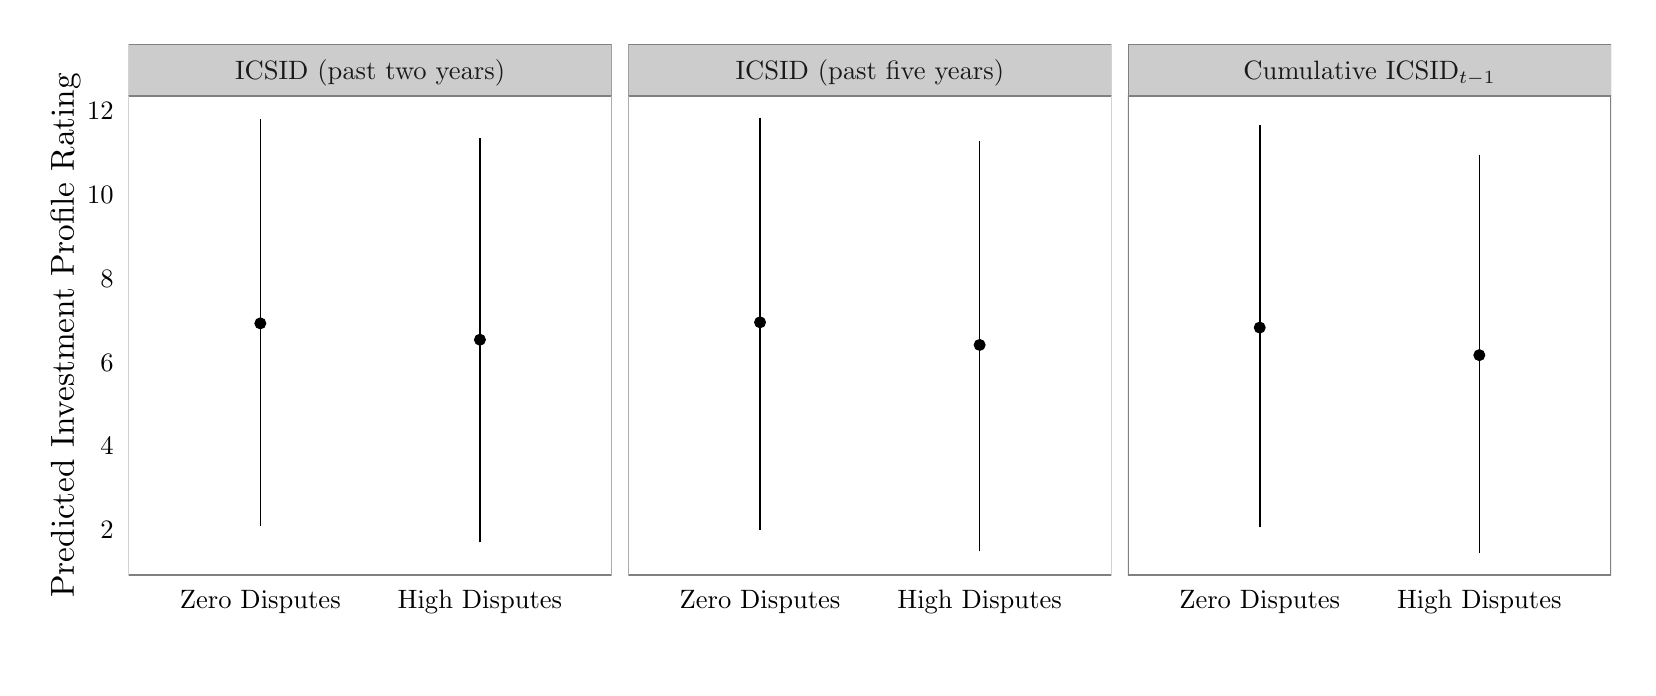
\begin{tikzpicture}[x=1pt,y=1pt]
\definecolor[named]{drawColor}{rgb}{0.00,0.00,0.00}
\definecolor[named]{fillColor}{rgb}{1.00,1.00,1.00}
\fill[color=fillColor,] (0,0) rectangle (578.16,231.26);
\begin{scope}
\path[clip] (  0.00,  0.00) rectangle (578.16,231.26);
\end{scope}
\begin{scope}
\path[clip] (  0.00,  0.00) rectangle (578.16,231.26);
\end{scope}
\begin{scope}
\path[clip] (  0.00,  0.00) rectangle (578.16,231.26);
\end{scope}
\begin{scope}
\path[clip] (  0.00,  0.00) rectangle (578.16,231.26);
\end{scope}
\begin{scope}
\path[clip] (  0.00,  0.00) rectangle (578.16,231.26);
\end{scope}
\begin{scope}
\path[clip] (  0.00,  0.00) rectangle (578.16,231.26);
\end{scope}
\begin{scope}
\path[clip] (  0.00,  0.00) rectangle (578.16,231.26);
\end{scope}
\begin{scope}
\path[clip] (  0.00,  0.00) rectangle (578.16,231.26);
\end{scope}
\begin{scope}
\path[clip] (  0.00,  0.00) rectangle (578.16,231.26);
\end{scope}
\begin{scope}
\path[clip] (  0.00,  0.00) rectangle (578.16,231.26);
\end{scope}
\begin{scope}
\path[clip] (  0.00,  0.00) rectangle (578.16,231.26);
\end{scope}
\begin{scope}
\path[clip] (  0.00,  0.00) rectangle (578.16,231.26);
\end{scope}
\begin{scope}
\path[clip] (  0.00,  0.00) rectangle (578.16,231.26);
\end{scope}
\begin{scope}
\path[clip] (  0.00,  0.00) rectangle (578.16,231.26);
\definecolor[named]{drawColor}{rgb}{1.00,1.00,1.00}
\definecolor[named]{fillColor}{rgb}{1.00,1.00,1.00}

\draw[color=drawColor,line width= 0.6pt,line cap=round,line join=round,fill=fillColor,] (  0.00,  0.00) rectangle (578.16,231.26);
\end{scope}
\begin{scope}
\path[clip] (  0.00,  0.00) rectangle (578.16,231.26);
\end{scope}
\begin{scope}
\path[clip] ( 36.46, 33.48) rectangle (211.03,206.65);
\definecolor[named]{fillColor}{rgb}{1.00,1.00,1.00}

\draw[fill=fillColor,draw opacity=0.00,] ( 36.46, 33.48) rectangle (211.03,206.65);
\definecolor[named]{drawColor}{rgb}{0.00,0.00,0.00}
\definecolor[named]{fillColor}{rgb}{0.00,0.00,0.00}

\draw[color=drawColor,line width= 0.6pt,line join=round,fill=fillColor,] ( 84.07, 51.23) -- ( 84.07,198.22);

\draw[color=drawColor,line width= 0.6pt,line join=round,fill=fillColor,] (163.42, 45.31) -- (163.42,191.56);

\draw[color=drawColor,line width= 0.4pt,line cap=round,line join=round,fill=fillColor,] ( 84.07,124.41) circle (  1.96);

\draw[color=drawColor,line width= 0.4pt,line cap=round,line join=round,fill=fillColor,] (163.42,118.50) circle (  1.96);
\definecolor[named]{drawColor}{rgb}{0.50,0.50,0.50}

\draw[color=drawColor,line width= 0.6pt,line cap=round,line join=round,fill opacity=0.00,] ( 36.46, 33.48) rectangle (211.03,206.65);
\end{scope}
\begin{scope}
\path[clip] (  0.00,  0.00) rectangle (578.16,231.26);
\end{scope}
\begin{scope}
\path[clip] (217.03, 33.48) rectangle (391.59,206.65);
\definecolor[named]{fillColor}{rgb}{1.00,1.00,1.00}

\draw[fill=fillColor,draw opacity=0.00,] (217.03, 33.48) rectangle (391.59,206.65);
\definecolor[named]{drawColor}{rgb}{0.00,0.00,0.00}
\definecolor[named]{fillColor}{rgb}{0.00,0.00,0.00}

\draw[color=drawColor,line width= 0.6pt,line join=round,fill=fillColor,] (264.64, 49.75) -- (264.64,198.78);

\draw[color=drawColor,line width= 0.6pt,line join=round,fill=fillColor,] (343.99, 42.06) -- (343.99,190.16);

\draw[color=drawColor,line width= 0.4pt,line cap=round,line join=round,fill=fillColor,] (264.64,124.79) circle (  1.96);

\draw[color=drawColor,line width= 0.4pt,line cap=round,line join=round,fill=fillColor,] (343.99,116.61) circle (  1.96);
\definecolor[named]{drawColor}{rgb}{0.50,0.50,0.50}

\draw[color=drawColor,line width= 0.6pt,line cap=round,line join=round,fill opacity=0.00,] (217.03, 33.48) rectangle (391.59,206.65);
\end{scope}
\begin{scope}
\path[clip] (  0.00,  0.00) rectangle (578.16,231.26);
\end{scope}
\begin{scope}
\path[clip] (397.59, 33.48) rectangle (572.16,206.65);
\definecolor[named]{fillColor}{rgb}{1.00,1.00,1.00}

\draw[fill=fillColor,draw opacity=0.00,] (397.59, 33.48) rectangle (572.16,206.65);
\definecolor[named]{drawColor}{rgb}{0.00,0.00,0.00}
\definecolor[named]{fillColor}{rgb}{0.00,0.00,0.00}

\draw[color=drawColor,line width= 0.6pt,line join=round,fill=fillColor,] (445.20, 50.70) -- (445.20,196.03);

\draw[color=drawColor,line width= 0.6pt,line join=round,fill=fillColor,] (524.55, 41.35) -- (524.55,185.34);

\draw[color=drawColor,line width= 0.4pt,line cap=round,line join=round,fill=fillColor,] (445.20,122.89) circle (  1.96);

\draw[color=drawColor,line width= 0.4pt,line cap=round,line join=round,fill=fillColor,] (524.55,112.93) circle (  1.96);
\definecolor[named]{drawColor}{rgb}{0.50,0.50,0.50}

\draw[color=drawColor,line width= 0.6pt,line cap=round,line join=round,fill opacity=0.00,] (397.59, 33.48) rectangle (572.16,206.65);
\end{scope}
\begin{scope}
\path[clip] (  0.00,  0.00) rectangle (578.16,231.26);
\end{scope}
\begin{scope}
\path[clip] (  0.00,  0.00) rectangle (578.16,231.26);
\end{scope}
\begin{scope}
\path[clip] (  0.00,  0.00) rectangle (578.16,231.26);
\end{scope}
\begin{scope}
\path[clip] ( 36.46,206.65) rectangle (211.03,225.26);
\definecolor[named]{drawColor}{rgb}{0.50,0.50,0.50}
\definecolor[named]{fillColor}{rgb}{0.80,0.80,0.80}

\draw[color=drawColor,line width= 0.2pt,line cap=round,line join=round,fill=fillColor,] ( 36.46,206.65) rectangle (211.03,225.26);
\definecolor[named]{drawColor}{rgb}{0.10,0.10,0.10}

\node[color=drawColor,anchor=base,inner sep=0pt, outer sep=0pt, scale=  0.96] at (123.75,212.65) {ICSID (past two years)%
};
\end{scope}
\begin{scope}
\path[clip] ( 36.46,206.65) rectangle (211.03,225.26);
\end{scope}
\begin{scope}
\path[clip] (  0.00,  0.00) rectangle (578.16,231.26);
\end{scope}
\begin{scope}
\path[clip] (  0.00,  0.00) rectangle (578.16,231.26);
\end{scope}
\begin{scope}
\path[clip] (  0.00,  0.00) rectangle (578.16,231.26);
\end{scope}
\begin{scope}
\path[clip] (  0.00,  0.00) rectangle (578.16,231.26);
\end{scope}
\begin{scope}
\path[clip] (  0.00,  0.00) rectangle (578.16,231.26);
\end{scope}
\begin{scope}
\path[clip] (  0.00,  0.00) rectangle (578.16,231.26);
\end{scope}
\begin{scope}
\path[clip] (217.03,206.65) rectangle (391.59,225.26);
\definecolor[named]{drawColor}{rgb}{0.50,0.50,0.50}
\definecolor[named]{fillColor}{rgb}{0.80,0.80,0.80}

\draw[color=drawColor,line width= 0.2pt,line cap=round,line join=round,fill=fillColor,] (217.03,206.65) rectangle (391.59,225.26);
\definecolor[named]{drawColor}{rgb}{0.10,0.10,0.10}

\node[color=drawColor,anchor=base,inner sep=0pt, outer sep=0pt, scale=  0.96] at (304.31,212.65) {ICSID (past five years)%
};
\end{scope}
\begin{scope}
\path[clip] (217.03,206.65) rectangle (391.59,225.26);
\end{scope}
\begin{scope}
\path[clip] (  0.00,  0.00) rectangle (578.16,231.26);
\end{scope}
\begin{scope}
\path[clip] (  0.00,  0.00) rectangle (578.16,231.26);
\end{scope}
\begin{scope}
\path[clip] (  0.00,  0.00) rectangle (578.16,231.26);
\end{scope}
\begin{scope}
\path[clip] (  0.00,  0.00) rectangle (578.16,231.26);
\end{scope}
\begin{scope}
\path[clip] (  0.00,  0.00) rectangle (578.16,231.26);
\end{scope}
\begin{scope}
\path[clip] (  0.00,  0.00) rectangle (578.16,231.26);
\end{scope}
\begin{scope}
\path[clip] (397.59,206.65) rectangle (572.16,225.26);
\definecolor[named]{drawColor}{rgb}{0.50,0.50,0.50}
\definecolor[named]{fillColor}{rgb}{0.80,0.80,0.80}

\draw[color=drawColor,line width= 0.2pt,line cap=round,line join=round,fill=fillColor,] (397.59,206.65) rectangle (572.16,225.26);
\definecolor[named]{drawColor}{rgb}{0.10,0.10,0.10}

\node[color=drawColor,anchor=base,inner sep=0pt, outer sep=0pt, scale=  0.96] at (484.88,212.65) {Cumulative ICSID$_{t-1}$%
};
\end{scope}
\begin{scope}
\path[clip] (397.59,206.65) rectangle (572.16,225.26);
\end{scope}
\begin{scope}
\path[clip] (  0.00,  0.00) rectangle (578.16,231.26);
\end{scope}
\begin{scope}
\path[clip] (  0.00,  0.00) rectangle (578.16,231.26);
\end{scope}
\begin{scope}
\path[clip] (  0.00,  0.00) rectangle (578.16,231.26);
\end{scope}
\begin{scope}
\path[clip] (  0.00,  0.00) rectangle (578.16,231.26);
\end{scope}
\begin{scope}
\path[clip] (  0.00,  0.00) rectangle (578.16,231.26);
\end{scope}
\begin{scope}
\path[clip] (  0.00,  0.00) rectangle (578.16,231.26);
\end{scope}
\begin{scope}
\path[clip] (  0.00,  0.00) rectangle (578.16,231.26);
\end{scope}
\begin{scope}
\path[clip] (  0.00,  0.00) rectangle (578.16,231.26);
\end{scope}
\begin{scope}
\path[clip] (  0.00,  0.00) rectangle (578.16,231.26);
\definecolor[named]{drawColor}{rgb}{0.00,0.00,0.00}

\node[color=drawColor,anchor=base east,inner sep=0pt, outer sep=0pt, scale=  0.96] at ( 31.06, 46.57) {2%
};

\node[color=drawColor,anchor=base east,inner sep=0pt, outer sep=0pt, scale=  0.96] at ( 31.06, 76.85) {4%
};

\node[color=drawColor,anchor=base east,inner sep=0pt, outer sep=0pt, scale=  0.96] at ( 31.06,107.14) {6%
};

\node[color=drawColor,anchor=base east,inner sep=0pt, outer sep=0pt, scale=  0.96] at ( 31.06,137.42) {8%
};

\node[color=drawColor,anchor=base east,inner sep=0pt, outer sep=0pt, scale=  0.96] at ( 31.06,167.70) {10%
};

\node[color=drawColor,anchor=base east,inner sep=0pt, outer sep=0pt, scale=  0.96] at ( 31.06,197.98) {12%
};
\end{scope}
\begin{scope}
\path[clip] (  0.00,  0.00) rectangle (578.16,231.26);
\end{scope}
\begin{scope}
\path[clip] (  0.00,  0.00) rectangle (578.16,231.26);
\end{scope}
\begin{scope}
\path[clip] (  0.00,  0.00) rectangle (578.16,231.26);
\end{scope}
\begin{scope}
\path[clip] (  0.00,  0.00) rectangle (578.16,231.26);
\end{scope}
\begin{scope}
\path[clip] (  0.00,  0.00) rectangle (578.16,231.26);
\end{scope}
\begin{scope}
\path[clip] (  0.00,  0.00) rectangle (578.16,231.26);
\end{scope}
\begin{scope}
\path[clip] (  0.00,  0.00) rectangle (578.16,231.26);
\end{scope}
\begin{scope}
\path[clip] (  0.00,  0.00) rectangle (578.16,231.26);
\end{scope}
\begin{scope}
\path[clip] (  0.00,  0.00) rectangle (578.16,231.26);
\end{scope}
\begin{scope}
\path[clip] (  0.00,  0.00) rectangle (578.16,231.26);
\end{scope}
\begin{scope}
\path[clip] (  0.00,  0.00) rectangle (578.16,231.26);
\end{scope}
\begin{scope}
\path[clip] (  0.00,  0.00) rectangle (578.16,231.26);
\end{scope}
\begin{scope}
\path[clip] (  0.00,  0.00) rectangle (578.16,231.26);
\end{scope}
\begin{scope}
\path[clip] (  0.00,  0.00) rectangle (578.16,231.26);
\end{scope}
\begin{scope}
\path[clip] (  0.00,  0.00) rectangle (578.16,231.26);
\end{scope}
\begin{scope}
\path[clip] (  0.00,  0.00) rectangle (578.16,231.26);
\end{scope}
\begin{scope}
\path[clip] (  0.00,  0.00) rectangle (578.16,231.26);
\end{scope}
\begin{scope}
\path[clip] (  0.00,  0.00) rectangle (578.16,231.26);
\definecolor[named]{drawColor}{rgb}{0.00,0.00,0.00}

\node[color=drawColor,anchor=base,inner sep=0pt, outer sep=0pt, scale=  0.96] at ( 84.07, 21.46) {Zero Disputes%
};

\node[color=drawColor,anchor=base,inner sep=0pt, outer sep=0pt, scale=  0.96] at (163.42, 21.46) {High Disputes%
};
\end{scope}
\begin{scope}
\path[clip] (  0.00,  0.00) rectangle (578.16,231.26);
\end{scope}
\begin{scope}
\path[clip] (  0.00,  0.00) rectangle (578.16,231.26);
\end{scope}
\begin{scope}
\path[clip] (  0.00,  0.00) rectangle (578.16,231.26);
\end{scope}
\begin{scope}
\path[clip] (  0.00,  0.00) rectangle (578.16,231.26);
\end{scope}
\begin{scope}
\path[clip] (  0.00,  0.00) rectangle (578.16,231.26);
\end{scope}
\begin{scope}
\path[clip] (  0.00,  0.00) rectangle (578.16,231.26);
\end{scope}
\begin{scope}
\path[clip] (  0.00,  0.00) rectangle (578.16,231.26);
\end{scope}
\begin{scope}
\path[clip] (  0.00,  0.00) rectangle (578.16,231.26);
\end{scope}
\begin{scope}
\path[clip] (  0.00,  0.00) rectangle (578.16,231.26);
\end{scope}
\begin{scope}
\path[clip] (  0.00,  0.00) rectangle (578.16,231.26);
\end{scope}
\begin{scope}
\path[clip] (  0.00,  0.00) rectangle (578.16,231.26);
\end{scope}
\begin{scope}
\path[clip] (  0.00,  0.00) rectangle (578.16,231.26);
\definecolor[named]{drawColor}{rgb}{0.00,0.00,0.00}

\node[color=drawColor,anchor=base,inner sep=0pt, outer sep=0pt, scale=  0.96] at (264.64, 21.46) {Zero Disputes%
};

\node[color=drawColor,anchor=base,inner sep=0pt, outer sep=0pt, scale=  0.96] at (343.99, 21.46) {High Disputes%
};
\end{scope}
\begin{scope}
\path[clip] (  0.00,  0.00) rectangle (578.16,231.26);
\end{scope}
\begin{scope}
\path[clip] (  0.00,  0.00) rectangle (578.16,231.26);
\end{scope}
\begin{scope}
\path[clip] (  0.00,  0.00) rectangle (578.16,231.26);
\end{scope}
\begin{scope}
\path[clip] (  0.00,  0.00) rectangle (578.16,231.26);
\end{scope}
\begin{scope}
\path[clip] (  0.00,  0.00) rectangle (578.16,231.26);
\end{scope}
\begin{scope}
\path[clip] (  0.00,  0.00) rectangle (578.16,231.26);
\end{scope}
\begin{scope}
\path[clip] (  0.00,  0.00) rectangle (578.16,231.26);
\end{scope}
\begin{scope}
\path[clip] (  0.00,  0.00) rectangle (578.16,231.26);
\end{scope}
\begin{scope}
\path[clip] (  0.00,  0.00) rectangle (578.16,231.26);
\end{scope}
\begin{scope}
\path[clip] (  0.00,  0.00) rectangle (578.16,231.26);
\end{scope}
\begin{scope}
\path[clip] (  0.00,  0.00) rectangle (578.16,231.26);
\end{scope}
\begin{scope}
\path[clip] (  0.00,  0.00) rectangle (578.16,231.26);
\definecolor[named]{drawColor}{rgb}{0.00,0.00,0.00}

\node[color=drawColor,anchor=base,inner sep=0pt, outer sep=0pt, scale=  0.96] at (445.20, 21.46) {Zero Disputes%
};

\node[color=drawColor,anchor=base,inner sep=0pt, outer sep=0pt, scale=  0.96] at (524.55, 21.46) {High Disputes%
};
\end{scope}
\begin{scope}
\path[clip] (  0.00,  0.00) rectangle (578.16,231.26);
\end{scope}
\begin{scope}
\path[clip] (  0.00,  0.00) rectangle (578.16,231.26);
\end{scope}
\begin{scope}
\path[clip] (  0.00,  0.00) rectangle (578.16,231.26);
\end{scope}
\begin{scope}
\path[clip] (  0.00,  0.00) rectangle (578.16,231.26);
\end{scope}
\begin{scope}
\path[clip] (  0.00,  0.00) rectangle (578.16,231.26);
\end{scope}
\begin{scope}
\path[clip] (  0.00,  0.00) rectangle (578.16,231.26);
\end{scope}
\begin{scope}
\path[clip] (  0.00,  0.00) rectangle (578.16,231.26);
\end{scope}
\begin{scope}
\path[clip] (  0.00,  0.00) rectangle (578.16,231.26);
\end{scope}
\begin{scope}
\path[clip] (  0.00,  0.00) rectangle (578.16,231.26);
\definecolor[named]{drawColor}{rgb}{0.00,0.00,0.00}

\node[rotate= 90.00,color=drawColor,anchor=base,inner sep=0pt, outer sep=0pt, scale=  1.20] at ( 16.66,120.06) {Predicted Investment Profile Rating%
};
\end{scope}
\begin{scope}
\path[clip] (  0.00,  0.00) rectangle (578.16,231.26);
\end{scope}
\begin{scope}
\path[clip] (  0.00,  0.00) rectangle (578.16,231.26);
\end{scope}
\begin{scope}
\path[clip] (  0.00,  0.00) rectangle (578.16,231.26);
\end{scope}
\begin{scope}
\path[clip] (  0.00,  0.00) rectangle (578.16,231.26);
\end{scope}
\begin{scope}
\path[clip] (  0.00,  0.00) rectangle (578.16,231.26);
\end{scope}
\end{tikzpicture}
}
	\caption*{Note: Here we show a typical country's predicted rating on investment profile under a scenario where a country faces a minimum versus the 99th percentile number of disputes, for each of the dispute variables this is equal to 3. Results were obtained by using simulations that accounted for inferential uncertainty. The point estimates here represent the mean predicted ratings and the line represents the 95\% level of uncertainty associated with these estimates.}
\end{figure}

% \newpage

However, the fact that the level of uncertainty around our predicted values is so high does raise an important and interesting question. As we discussed earlier, the assumption that international institutions will instantly be able to generate adverse effects with regards to country reputation is questionable. Allee and Peinhardt assume that being taken in front of ICSID will lead to an almost immediate shift in how FDI flows will then change, but the implicit assumption there is that the credibility and awareness of ICSID has been constant over time. This is an unnecessary assumption that should be more closely examined by unpacking potential temporal variation in the effect that ICSID disputes have on a country's reputation for the protection of foreign investment.

To explore this issue, we rerun the analysis shown in table \ref{tab:dispRepLevel} on a series of yearly level pooled models between 1995 to 2011.\footnote{We begin our period for analysis here at 1995 because the infrequency of disputes before that date leads to cases in which no country had a dispute within the last two years.} All the control variables that we used in table \ref{tab:dispRepLevel} are used here as well. For the sake of space, since our substantive interest is in how the effect of disputes has changed over time, we only show the coefficient results for our dispute measures. Figure \ref{fig:dispEffectYear} shows the results of this analysis, the dot in each line represents the coefficient estimate for a disputes variable in that year, and the line width represents the 95 percent confidence interval around that point estimate. Coefficient estimates that are significant at a 95 percent confidence interval are colored in dark grey. 

Interestingly, we find significant variation in how the effect of disputes on reputation has changed over time. Prior to 2007, the estimated effect of dispute initiations on reputation is quite imprecisely measured. After that point, the precision of the estimated effect narrows dramatically, and across each dispute variable there exists a clear negative relationship between the initiation of disputes within the past two years and perceptions of a country's reputation with regards to the protection of investment. 

\begin{figure}[ht]
	\vspace{4cm}
	\centering
	\caption{Change in Effect of Disputes Over Time}
	\label{fig:dispEffectYear}
	\resizebox{1\textwidth}{!}{% Created by tikzDevice version 0.7.0 on 2015-01-17 17:55:38
% !TEX encoding = UTF-8 Unicode
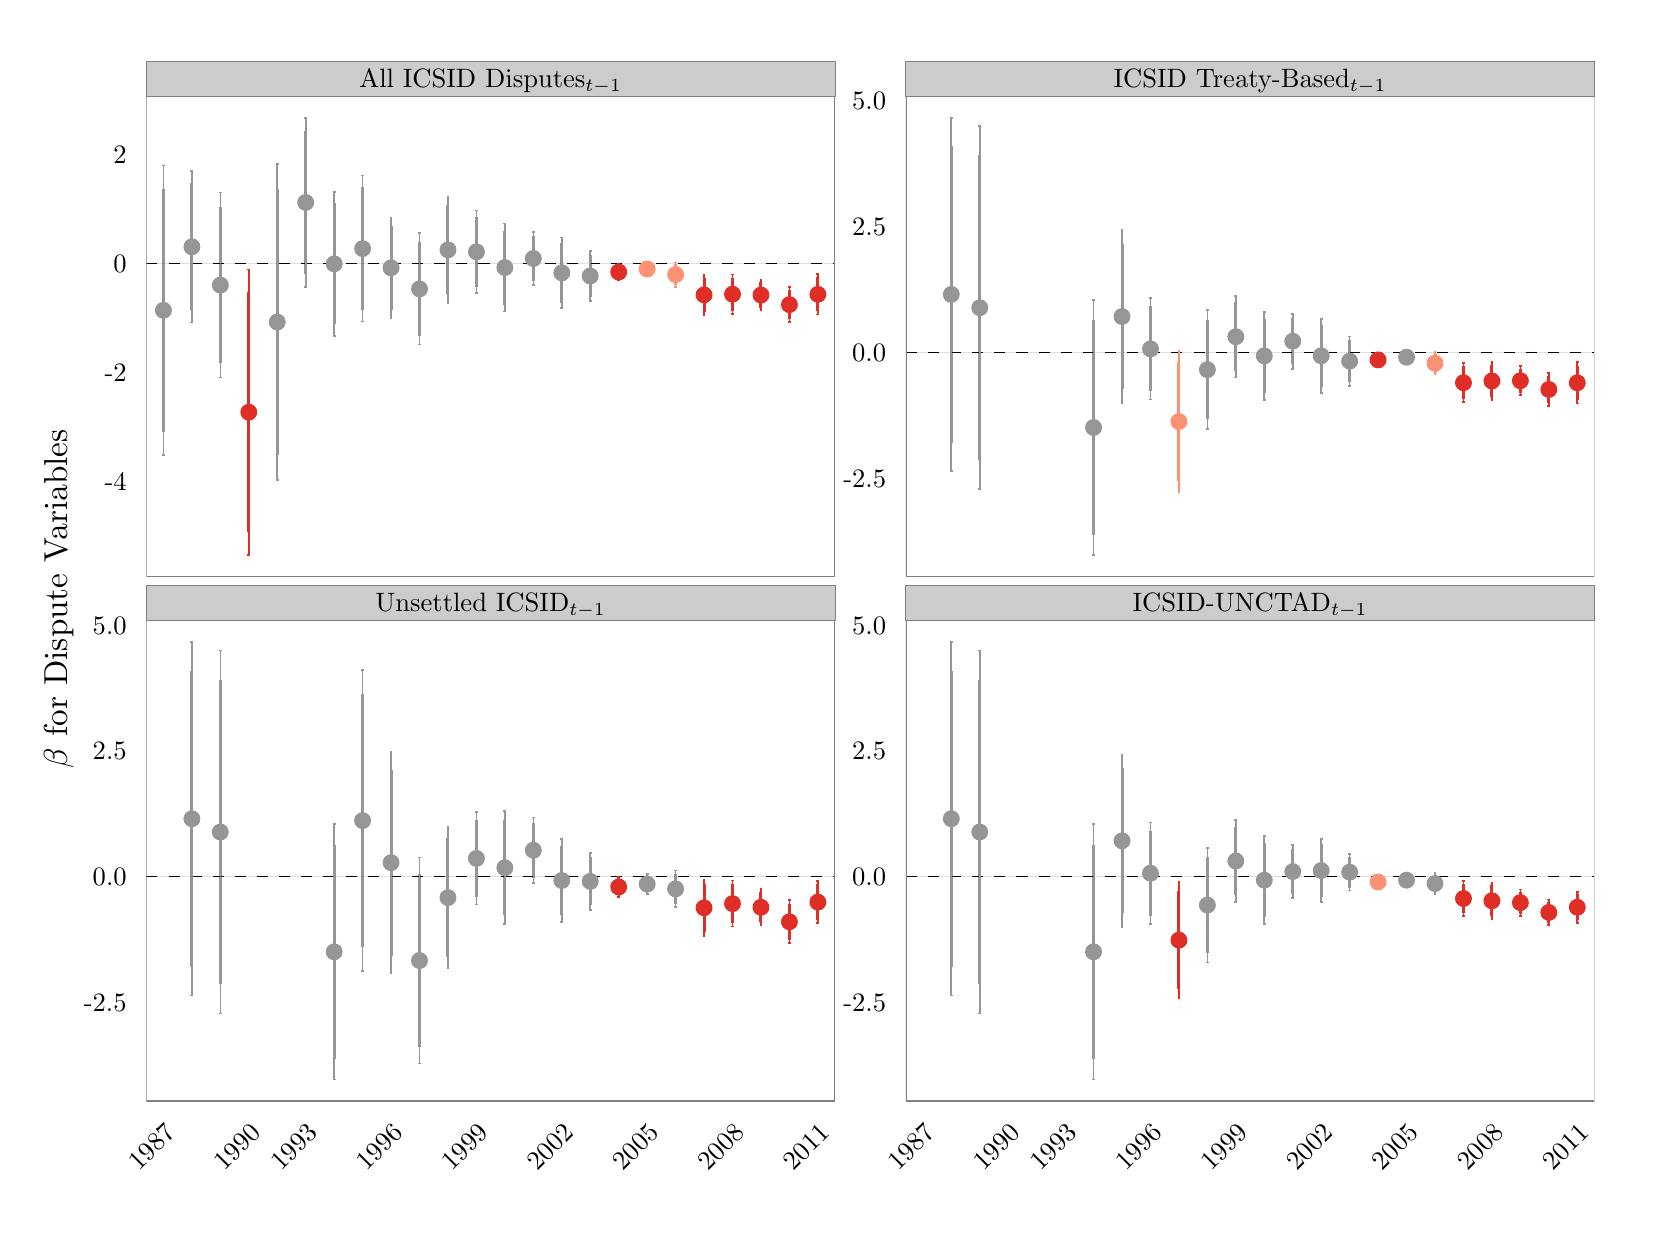
\begin{tikzpicture}[x=1pt,y=1pt]
\definecolor[named]{fillColor}{rgb}{1.00,1.00,1.00}
\path[use as bounding box,fill=fillColor,fill opacity=0.00] (0,0) rectangle (578.16,433.62);
\begin{scope}
\path[clip] (  0.00,  0.00) rectangle (578.16,433.62);
\definecolor[named]{drawColor}{rgb}{1.00,1.00,1.00}
\definecolor[named]{fillColor}{rgb}{1.00,1.00,1.00}

\path[draw=drawColor,line width= 0.6pt,line join=round,line cap=round,fill=fillColor] (  0.00,  0.00) rectangle (578.16,433.62);
\end{scope}
\begin{scope}
\path[clip] ( 42.89,235.13) rectangle (291.71,408.94);
\definecolor[named]{fillColor}{rgb}{1.00,1.00,1.00}

\path[fill=fillColor] ( 42.89,235.13) rectangle (291.71,408.94);
\definecolor[named]{drawColor}{rgb}{0.59,0.59,0.59}
\definecolor[named]{fillColor}{rgb}{0.59,0.59,0.59}

\path[draw=drawColor,draw opacity=0.30,line width= 0.3pt,line join=round,fill=fillColor,fill opacity=0.30] ( 49.05,279.17) -- ( 49.05,383.79);

\path[draw=drawColor,draw opacity=0.30,line width= 0.3pt,line join=round,fill=fillColor,fill opacity=0.30] ( 59.34,327.06) -- ( 59.34,381.80);

\path[draw=drawColor,draw opacity=0.30,line width= 0.3pt,line join=round,fill=fillColor,fill opacity=0.30] ( 69.62,307.18) -- ( 69.62,374.02);
\definecolor[named]{drawColor}{rgb}{0.87,0.18,0.15}
\definecolor[named]{fillColor}{rgb}{0.87,0.18,0.15}

\path[draw=drawColor,draw opacity=0.30,line width= 0.3pt,line join=round,fill=fillColor,fill opacity=0.30] ( 79.90,243.03) -- ( 79.90,346.28);
\definecolor[named]{drawColor}{rgb}{0.59,0.59,0.59}
\definecolor[named]{fillColor}{rgb}{0.59,0.59,0.59}

\path[draw=drawColor,draw opacity=0.30,line width= 0.3pt,line join=round,fill=fillColor,fill opacity=0.30] ( 90.18,270.12) -- ( 90.18,384.39);

\path[draw=drawColor,draw opacity=0.30,line width= 0.3pt,line join=round,fill=fillColor,fill opacity=0.30] (100.46,339.87) -- (100.46,401.04);

\path[draw=drawColor,draw opacity=0.30,line width= 0.3pt,line join=round,fill=fillColor,fill opacity=0.30] (110.75,322.30) -- (110.75,374.27);

\path[draw=drawColor,draw opacity=0.30,line width= 0.3pt,line join=round,fill=fillColor,fill opacity=0.30] (121.03,327.40) -- (121.03,380.17);

\path[draw=drawColor,draw opacity=0.30,line width= 0.3pt,line join=round,fill=fillColor,fill opacity=0.30] (131.31,328.76) -- (131.31,364.94);

\path[draw=drawColor,draw opacity=0.30,line width= 0.3pt,line join=round,fill=fillColor,fill opacity=0.30] (141.59,319.07) -- (141.59,359.35);

\path[draw=drawColor,draw opacity=0.30,line width= 0.3pt,line join=round,fill=fillColor,fill opacity=0.30] (151.87,334.15) -- (151.87,372.51);

\path[draw=drawColor,draw opacity=0.30,line width= 0.3pt,line join=round,fill=fillColor,fill opacity=0.30] (162.16,337.67) -- (162.16,367.57);

\path[draw=drawColor,draw opacity=0.30,line width= 0.3pt,line join=round,fill=fillColor,fill opacity=0.30] (172.44,331.01) -- (172.44,362.86);

\path[draw=drawColor,draw opacity=0.30,line width= 0.3pt,line join=round,fill=fillColor,fill opacity=0.30] (182.72,340.60) -- (182.72,359.82);

\path[draw=drawColor,draw opacity=0.30,line width= 0.3pt,line join=round,fill=fillColor,fill opacity=0.30] (193.00,332.20) -- (193.00,357.84);

\path[draw=drawColor,draw opacity=0.30,line width= 0.3pt,line join=round,fill=fillColor,fill opacity=0.30] (203.28,334.77) -- (203.28,352.99);
\definecolor[named]{drawColor}{rgb}{0.87,0.18,0.15}
\definecolor[named]{fillColor}{rgb}{0.87,0.18,0.15}

\path[draw=drawColor,draw opacity=0.30,line width= 0.3pt,line join=round,fill=fillColor,fill opacity=0.30] (213.56,342.52) -- (213.56,348.12);
\definecolor[named]{drawColor}{rgb}{0.99,0.57,0.45}
\definecolor[named]{fillColor}{rgb}{0.99,0.57,0.45}

\path[draw=drawColor,draw opacity=0.30,line width= 0.3pt,line join=round,fill=fillColor,fill opacity=0.30] (223.85,344.07) -- (223.85,348.80);

\path[draw=drawColor,draw opacity=0.30,line width= 0.3pt,line join=round,fill=fillColor,fill opacity=0.30] (234.13,339.99) -- (234.13,348.81);
\definecolor[named]{drawColor}{rgb}{0.87,0.18,0.15}
\definecolor[named]{fillColor}{rgb}{0.87,0.18,0.15}

\path[draw=drawColor,draw opacity=0.30,line width= 0.3pt,line join=round,fill=fillColor,fill opacity=0.30] (244.41,329.66) -- (244.41,344.47);

\path[draw=drawColor,draw opacity=0.30,line width= 0.3pt,line join=round,fill=fillColor,fill opacity=0.30] (254.69,330.17) -- (254.69,344.45);

\path[draw=drawColor,draw opacity=0.30,line width= 0.3pt,line join=round,fill=fillColor,fill opacity=0.30] (264.97,331.37) -- (264.97,342.62);

\path[draw=drawColor,draw opacity=0.30,line width= 0.3pt,line join=round,fill=fillColor,fill opacity=0.30] (275.26,327.22) -- (275.26,339.84);

\path[draw=drawColor,draw opacity=0.30,line width= 0.3pt,line join=round,fill=fillColor,fill opacity=0.30] (285.54,329.97) -- (285.54,344.55);
\definecolor[named]{drawColor}{rgb}{0.59,0.59,0.59}
\definecolor[named]{fillColor}{rgb}{0.59,0.59,0.59}

\path[draw=drawColor,line width= 1.1pt,line join=round,fill=fillColor] ( 49.05,287.58) -- ( 49.05,375.38);

\path[draw=drawColor,line width= 1.1pt,line join=round,fill=fillColor] ( 59.34,331.46) -- ( 59.34,377.40);

\path[draw=drawColor,line width= 1.1pt,line join=round,fill=fillColor] ( 69.62,312.55) -- ( 69.62,368.65);
\definecolor[named]{drawColor}{rgb}{0.87,0.18,0.15}
\definecolor[named]{fillColor}{rgb}{0.87,0.18,0.15}

\path[draw=drawColor,line width= 1.1pt,line join=round,fill=fillColor] ( 79.90,251.33) -- ( 79.90,337.98);
\definecolor[named]{drawColor}{rgb}{0.59,0.59,0.59}
\definecolor[named]{fillColor}{rgb}{0.59,0.59,0.59}

\path[draw=drawColor,line width= 1.1pt,line join=round,fill=fillColor] ( 90.18,279.30) -- ( 90.18,375.20);

\path[draw=drawColor,line width= 1.1pt,line join=round,fill=fillColor] (100.46,344.78) -- (100.46,396.12);

\path[draw=drawColor,line width= 1.1pt,line join=round,fill=fillColor] (110.75,326.48) -- (110.75,370.09);

\path[draw=drawColor,line width= 1.1pt,line join=round,fill=fillColor] (121.03,331.64) -- (121.03,375.93);

\path[draw=drawColor,line width= 1.1pt,line join=round,fill=fillColor] (131.31,331.67) -- (131.31,362.03);

\path[draw=drawColor,line width= 1.1pt,line join=round,fill=fillColor] (141.59,322.31) -- (141.59,356.11);

\path[draw=drawColor,line width= 1.1pt,line join=round,fill=fillColor] (151.87,337.23) -- (151.87,369.43);

\path[draw=drawColor,line width= 1.1pt,line join=round,fill=fillColor] (162.16,340.07) -- (162.16,365.17);

\path[draw=drawColor,line width= 1.1pt,line join=round,fill=fillColor] (172.44,333.57) -- (172.44,360.30);

\path[draw=drawColor,line width= 1.1pt,line join=round,fill=fillColor] (182.72,342.14) -- (182.72,358.27);

\path[draw=drawColor,line width= 1.1pt,line join=round,fill=fillColor] (193.00,334.26) -- (193.00,355.78);

\path[draw=drawColor,line width= 1.1pt,line join=round,fill=fillColor] (203.28,336.24) -- (203.28,351.52);
\definecolor[named]{drawColor}{rgb}{0.87,0.18,0.15}
\definecolor[named]{fillColor}{rgb}{0.87,0.18,0.15}

\path[draw=drawColor,line width= 1.1pt,line join=round,fill=fillColor] (213.56,342.97) -- (213.56,347.67);
\definecolor[named]{drawColor}{rgb}{0.99,0.57,0.45}
\definecolor[named]{fillColor}{rgb}{0.99,0.57,0.45}

\path[draw=drawColor,line width= 1.1pt,line join=round,fill=fillColor] (223.85,344.45) -- (223.85,348.42);

\path[draw=drawColor,line width= 1.1pt,line join=round,fill=fillColor] (234.13,340.70) -- (234.13,348.10);
\definecolor[named]{drawColor}{rgb}{0.87,0.18,0.15}
\definecolor[named]{fillColor}{rgb}{0.87,0.18,0.15}

\path[draw=drawColor,line width= 1.1pt,line join=round,fill=fillColor] (244.41,330.85) -- (244.41,343.28);

\path[draw=drawColor,line width= 1.1pt,line join=round,fill=fillColor] (254.69,331.32) -- (254.69,343.30);

\path[draw=drawColor,line width= 1.1pt,line join=round,fill=fillColor] (264.97,332.28) -- (264.97,341.71);

\path[draw=drawColor,line width= 1.1pt,line join=round,fill=fillColor] (275.26,328.24) -- (275.26,338.83);

\path[draw=drawColor,line width= 1.1pt,line join=round,fill=fillColor] (285.54,331.14) -- (285.54,343.38);
\definecolor[named]{drawColor}{rgb}{0.00,0.00,0.00}
\definecolor[named]{fillColor}{rgb}{0.00,0.00,0.00}

\path[draw=drawColor,line width= 0.6pt,dash pattern=on 4pt off 4pt ,line join=round,fill=fillColor] ( 42.89,348.44) -- (291.71,348.44);
\definecolor[named]{drawColor}{rgb}{0.59,0.59,0.59}
\definecolor[named]{fillColor}{rgb}{0.59,0.59,0.59}

\path[draw=drawColor,line width= 0.4pt,line join=round,line cap=round,fill=fillColor] ( 49.05,331.48) circle (  2.85);

\path[draw=drawColor,line width= 0.4pt,line join=round,line cap=round,fill=fillColor] ( 59.34,354.43) circle (  2.85);

\path[draw=drawColor,line width= 0.4pt,line join=round,line cap=round,fill=fillColor] ( 69.62,340.60) circle (  2.85);
\definecolor[named]{drawColor}{rgb}{0.87,0.18,0.15}
\definecolor[named]{fillColor}{rgb}{0.87,0.18,0.15}

\path[draw=drawColor,line width= 0.4pt,line join=round,line cap=round,fill=fillColor] ( 79.90,294.66) circle (  2.85);
\definecolor[named]{drawColor}{rgb}{0.59,0.59,0.59}
\definecolor[named]{fillColor}{rgb}{0.59,0.59,0.59}

\path[draw=drawColor,line width= 0.4pt,line join=round,line cap=round,fill=fillColor] ( 90.18,327.25) circle (  2.85);

\path[draw=drawColor,line width= 0.4pt,line join=round,line cap=round,fill=fillColor] (100.46,370.45) circle (  2.85);

\path[draw=drawColor,line width= 0.4pt,line join=round,line cap=round,fill=fillColor] (110.75,348.28) circle (  2.85);

\path[draw=drawColor,line width= 0.4pt,line join=round,line cap=round,fill=fillColor] (121.03,353.79) circle (  2.85);

\path[draw=drawColor,line width= 0.4pt,line join=round,line cap=round,fill=fillColor] (131.31,346.85) circle (  2.85);

\path[draw=drawColor,line width= 0.4pt,line join=round,line cap=round,fill=fillColor] (141.59,339.21) circle (  2.85);

\path[draw=drawColor,line width= 0.4pt,line join=round,line cap=round,fill=fillColor] (151.87,353.33) circle (  2.85);

\path[draw=drawColor,line width= 0.4pt,line join=round,line cap=round,fill=fillColor] (162.16,352.62) circle (  2.85);

\path[draw=drawColor,line width= 0.4pt,line join=round,line cap=round,fill=fillColor] (172.44,346.94) circle (  2.85);

\path[draw=drawColor,line width= 0.4pt,line join=round,line cap=round,fill=fillColor] (182.72,350.21) circle (  2.85);

\path[draw=drawColor,line width= 0.4pt,line join=round,line cap=round,fill=fillColor] (193.00,345.02) circle (  2.85);

\path[draw=drawColor,line width= 0.4pt,line join=round,line cap=round,fill=fillColor] (203.28,343.88) circle (  2.85);
\definecolor[named]{drawColor}{rgb}{0.87,0.18,0.15}
\definecolor[named]{fillColor}{rgb}{0.87,0.18,0.15}

\path[draw=drawColor,line width= 0.4pt,line join=round,line cap=round,fill=fillColor] (213.56,345.32) circle (  2.85);
\definecolor[named]{drawColor}{rgb}{0.99,0.57,0.45}
\definecolor[named]{fillColor}{rgb}{0.99,0.57,0.45}

\path[draw=drawColor,line width= 0.4pt,line join=round,line cap=round,fill=fillColor] (223.85,346.43) circle (  2.85);

\path[draw=drawColor,line width= 0.4pt,line join=round,line cap=round,fill=fillColor] (234.13,344.40) circle (  2.85);
\definecolor[named]{drawColor}{rgb}{0.87,0.18,0.15}
\definecolor[named]{fillColor}{rgb}{0.87,0.18,0.15}

\path[draw=drawColor,line width= 0.4pt,line join=round,line cap=round,fill=fillColor] (244.41,337.07) circle (  2.85);

\path[draw=drawColor,line width= 0.4pt,line join=round,line cap=round,fill=fillColor] (254.69,337.31) circle (  2.85);

\path[draw=drawColor,line width= 0.4pt,line join=round,line cap=round,fill=fillColor] (264.97,337.00) circle (  2.85);

\path[draw=drawColor,line width= 0.4pt,line join=round,line cap=round,fill=fillColor] (275.26,333.53) circle (  2.85);

\path[draw=drawColor,line width= 0.4pt,line join=round,line cap=round,fill=fillColor] (285.54,337.26) circle (  2.85);
\definecolor[named]{drawColor}{rgb}{0.59,0.59,0.59}

\path[draw=drawColor,line width= 0.6pt,line join=round] ( 48.54,383.79) --
	( 49.57,383.79);

\path[draw=drawColor,line width= 0.6pt,line join=round] ( 49.05,383.79) --
	( 49.05,279.17);

\path[draw=drawColor,line width= 0.6pt,line join=round] ( 48.54,279.17) --
	( 49.57,279.17);

\path[draw=drawColor,line width= 0.6pt,line join=round] ( 58.82,381.80) --
	( 59.85,381.80);

\path[draw=drawColor,line width= 0.6pt,line join=round] ( 59.34,381.80) --
	( 59.34,327.06);

\path[draw=drawColor,line width= 0.6pt,line join=round] ( 58.82,327.06) --
	( 59.85,327.06);

\path[draw=drawColor,line width= 0.6pt,line join=round] ( 69.10,374.02) --
	( 70.13,374.02);

\path[draw=drawColor,line width= 0.6pt,line join=round] ( 69.62,374.02) --
	( 69.62,307.18);

\path[draw=drawColor,line width= 0.6pt,line join=round] ( 69.10,307.18) --
	( 70.13,307.18);
\definecolor[named]{drawColor}{rgb}{0.87,0.18,0.15}

\path[draw=drawColor,line width= 0.6pt,line join=round] ( 79.39,346.28) --
	( 80.41,346.28);

\path[draw=drawColor,line width= 0.6pt,line join=round] ( 79.90,346.28) --
	( 79.90,243.03);

\path[draw=drawColor,line width= 0.6pt,line join=round] ( 79.39,243.03) --
	( 80.41,243.03);
\definecolor[named]{drawColor}{rgb}{0.59,0.59,0.59}

\path[draw=drawColor,line width= 0.6pt,line join=round] ( 89.67,384.39) --
	( 90.70,384.39);

\path[draw=drawColor,line width= 0.6pt,line join=round] ( 90.18,384.39) --
	( 90.18,270.12);

\path[draw=drawColor,line width= 0.6pt,line join=round] ( 89.67,270.12) --
	( 90.70,270.12);

\path[draw=drawColor,line width= 0.6pt,line join=round] ( 99.95,401.04) --
	(100.98,401.04);

\path[draw=drawColor,line width= 0.6pt,line join=round] (100.46,401.04) --
	(100.46,339.87);

\path[draw=drawColor,line width= 0.6pt,line join=round] ( 99.95,339.87) --
	(100.98,339.87);

\path[draw=drawColor,line width= 0.6pt,line join=round] (110.23,374.27) --
	(111.26,374.27);

\path[draw=drawColor,line width= 0.6pt,line join=round] (110.75,374.27) --
	(110.75,322.30);

\path[draw=drawColor,line width= 0.6pt,line join=round] (110.23,322.30) --
	(111.26,322.30);

\path[draw=drawColor,line width= 0.6pt,line join=round] (120.51,380.17) --
	(121.54,380.17);

\path[draw=drawColor,line width= 0.6pt,line join=round] (121.03,380.17) --
	(121.03,327.40);

\path[draw=drawColor,line width= 0.6pt,line join=round] (120.51,327.40) --
	(121.54,327.40);

\path[draw=drawColor,line width= 0.6pt,line join=round] (130.80,364.94) --
	(131.82,364.94);

\path[draw=drawColor,line width= 0.6pt,line join=round] (131.31,364.94) --
	(131.31,328.76);

\path[draw=drawColor,line width= 0.6pt,line join=round] (130.80,328.76) --
	(131.82,328.76);

\path[draw=drawColor,line width= 0.6pt,line join=round] (141.08,359.35) --
	(142.11,359.35);

\path[draw=drawColor,line width= 0.6pt,line join=round] (141.59,359.35) --
	(141.59,319.07);

\path[draw=drawColor,line width= 0.6pt,line join=round] (141.08,319.07) --
	(142.11,319.07);

\path[draw=drawColor,line width= 0.6pt,line join=round] (151.36,372.51) --
	(152.39,372.51);

\path[draw=drawColor,line width= 0.6pt,line join=round] (151.87,372.51) --
	(151.87,334.15);

\path[draw=drawColor,line width= 0.6pt,line join=round] (151.36,334.15) --
	(152.39,334.15);

\path[draw=drawColor,line width= 0.6pt,line join=round] (161.64,367.57) --
	(162.67,367.57);

\path[draw=drawColor,line width= 0.6pt,line join=round] (162.16,367.57) --
	(162.16,337.67);

\path[draw=drawColor,line width= 0.6pt,line join=round] (161.64,337.67) --
	(162.67,337.67);

\path[draw=drawColor,line width= 0.6pt,line join=round] (171.92,362.86) --
	(172.95,362.86);

\path[draw=drawColor,line width= 0.6pt,line join=round] (172.44,362.86) --
	(172.44,331.01);

\path[draw=drawColor,line width= 0.6pt,line join=round] (171.92,331.01) --
	(172.95,331.01);

\path[draw=drawColor,line width= 0.6pt,line join=round] (182.20,359.82) --
	(183.23,359.82);

\path[draw=drawColor,line width= 0.6pt,line join=round] (182.72,359.82) --
	(182.72,340.60);

\path[draw=drawColor,line width= 0.6pt,line join=round] (182.20,340.60) --
	(183.23,340.60);

\path[draw=drawColor,line width= 0.6pt,line join=round] (192.49,357.84) --
	(193.51,357.84);

\path[draw=drawColor,line width= 0.6pt,line join=round] (193.00,357.84) --
	(193.00,332.20);

\path[draw=drawColor,line width= 0.6pt,line join=round] (192.49,332.20) --
	(193.51,332.20);

\path[draw=drawColor,line width= 0.6pt,line join=round] (202.77,352.99) --
	(203.80,352.99);

\path[draw=drawColor,line width= 0.6pt,line join=round] (203.28,352.99) --
	(203.28,334.77);

\path[draw=drawColor,line width= 0.6pt,line join=round] (202.77,334.77) --
	(203.80,334.77);
\definecolor[named]{drawColor}{rgb}{0.87,0.18,0.15}

\path[draw=drawColor,line width= 0.6pt,line join=round] (213.05,348.12) --
	(214.08,348.12);

\path[draw=drawColor,line width= 0.6pt,line join=round] (213.56,348.12) --
	(213.56,342.52);

\path[draw=drawColor,line width= 0.6pt,line join=round] (213.05,342.52) --
	(214.08,342.52);
\definecolor[named]{drawColor}{rgb}{0.99,0.57,0.45}

\path[draw=drawColor,line width= 0.6pt,line join=round] (223.33,348.80) --
	(224.36,348.80);

\path[draw=drawColor,line width= 0.6pt,line join=round] (223.85,348.80) --
	(223.85,344.07);

\path[draw=drawColor,line width= 0.6pt,line join=round] (223.33,344.07) --
	(224.36,344.07);

\path[draw=drawColor,line width= 0.6pt,line join=round] (233.61,348.81) --
	(234.64,348.81);

\path[draw=drawColor,line width= 0.6pt,line join=round] (234.13,348.81) --
	(234.13,339.99);

\path[draw=drawColor,line width= 0.6pt,line join=round] (233.61,339.99) --
	(234.64,339.99);
\definecolor[named]{drawColor}{rgb}{0.87,0.18,0.15}

\path[draw=drawColor,line width= 0.6pt,line join=round] (243.90,344.47) --
	(244.92,344.47);

\path[draw=drawColor,line width= 0.6pt,line join=round] (244.41,344.47) --
	(244.41,329.66);

\path[draw=drawColor,line width= 0.6pt,line join=round] (243.90,329.66) --
	(244.92,329.66);

\path[draw=drawColor,line width= 0.6pt,line join=round] (254.18,344.45) --
	(255.21,344.45);

\path[draw=drawColor,line width= 0.6pt,line join=round] (254.69,344.45) --
	(254.69,330.17);

\path[draw=drawColor,line width= 0.6pt,line join=round] (254.18,330.17) --
	(255.21,330.17);

\path[draw=drawColor,line width= 0.6pt,line join=round] (264.46,342.62) --
	(265.49,342.62);

\path[draw=drawColor,line width= 0.6pt,line join=round] (264.97,342.62) --
	(264.97,331.37);

\path[draw=drawColor,line width= 0.6pt,line join=round] (264.46,331.37) --
	(265.49,331.37);

\path[draw=drawColor,line width= 0.6pt,line join=round] (274.74,339.84) --
	(275.77,339.84);

\path[draw=drawColor,line width= 0.6pt,line join=round] (275.26,339.84) --
	(275.26,327.22);

\path[draw=drawColor,line width= 0.6pt,line join=round] (274.74,327.22) --
	(275.77,327.22);

\path[draw=drawColor,line width= 0.6pt,line join=round] (285.02,344.55) --
	(286.05,344.55);

\path[draw=drawColor,line width= 0.6pt,line join=round] (285.54,344.55) --
	(285.54,329.97);

\path[draw=drawColor,line width= 0.6pt,line join=round] (285.02,329.97) --
	(286.05,329.97);
\definecolor[named]{drawColor}{rgb}{0.50,0.50,0.50}

\path[draw=drawColor,line width= 0.6pt,line join=round,line cap=round] ( 42.89,235.13) rectangle (291.71,408.94);
\end{scope}
\begin{scope}
\path[clip] (317.29,235.13) rectangle (566.11,408.94);
\definecolor[named]{fillColor}{rgb}{1.00,1.00,1.00}

\path[fill=fillColor] (317.29,235.13) rectangle (566.11,408.94);
\definecolor[named]{drawColor}{rgb}{0.59,0.59,0.59}
\definecolor[named]{fillColor}{rgb}{0.59,0.59,0.59}

\path[draw=drawColor,draw opacity=0.30,line width= 0.3pt,line join=round,fill=fillColor,fill opacity=0.30] (333.75,273.40) -- (333.75,401.04);

\path[draw=drawColor,draw opacity=0.30,line width= 0.3pt,line join=round,fill=fillColor,fill opacity=0.30] (344.03,266.82) -- (344.03,398.03);

\path[draw=drawColor,draw opacity=0.30,line width= 0.3pt,line join=round,fill=fillColor,fill opacity=0.30] (385.15,243.03) -- (385.15,335.26);

\path[draw=drawColor,draw opacity=0.30,line width= 0.3pt,line join=round,fill=fillColor,fill opacity=0.30] (395.44,298.04) -- (395.44,360.45);

\path[draw=drawColor,draw opacity=0.30,line width= 0.3pt,line join=round,fill=fillColor,fill opacity=0.30] (405.72,299.23) -- (405.72,335.84);
\definecolor[named]{drawColor}{rgb}{0.99,0.57,0.45}
\definecolor[named]{fillColor}{rgb}{0.99,0.57,0.45}

\path[draw=drawColor,draw opacity=0.30,line width= 0.3pt,line join=round,fill=fillColor,fill opacity=0.30] (416.00,265.74) -- (416.00,316.84);
\definecolor[named]{drawColor}{rgb}{0.59,0.59,0.59}
\definecolor[named]{fillColor}{rgb}{0.59,0.59,0.59}

\path[draw=drawColor,draw opacity=0.30,line width= 0.3pt,line join=round,fill=fillColor,fill opacity=0.30] (426.28,288.61) -- (426.28,331.49);

\path[draw=drawColor,draw opacity=0.30,line width= 0.3pt,line join=round,fill=fillColor,fill opacity=0.30] (436.56,307.16) -- (436.56,336.74);

\path[draw=drawColor,draw opacity=0.30,line width= 0.3pt,line join=round,fill=fillColor,fill opacity=0.30] (446.85,299.07) -- (446.85,330.96);

\path[draw=drawColor,draw opacity=0.30,line width= 0.3pt,line join=round,fill=fillColor,fill opacity=0.30] (457.13,310.39) -- (457.13,330.24);

\path[draw=drawColor,draw opacity=0.30,line width= 0.3pt,line join=round,fill=fillColor,fill opacity=0.30] (467.41,301.67) -- (467.41,328.40);

\path[draw=drawColor,draw opacity=0.30,line width= 0.3pt,line join=round,fill=fillColor,fill opacity=0.30] (477.69,304.19) -- (477.69,322.08);
\definecolor[named]{drawColor}{rgb}{0.87,0.18,0.15}
\definecolor[named]{fillColor}{rgb}{0.87,0.18,0.15}

\path[draw=drawColor,draw opacity=0.30,line width= 0.3pt,line join=round,fill=fillColor,fill opacity=0.30] (487.97,310.97) -- (487.97,316.17);
\definecolor[named]{drawColor}{rgb}{0.59,0.59,0.59}
\definecolor[named]{fillColor}{rgb}{0.59,0.59,0.59}

\path[draw=drawColor,draw opacity=0.30,line width= 0.3pt,line join=round,fill=fillColor,fill opacity=0.30] (498.25,312.34) -- (498.25,316.74);
\definecolor[named]{drawColor}{rgb}{0.99,0.57,0.45}
\definecolor[named]{fillColor}{rgb}{0.99,0.57,0.45}

\path[draw=drawColor,draw opacity=0.30,line width= 0.3pt,line join=round,fill=fillColor,fill opacity=0.30] (508.54,308.23) -- (508.54,316.49);
\definecolor[named]{drawColor}{rgb}{0.87,0.18,0.15}
\definecolor[named]{fillColor}{rgb}{0.87,0.18,0.15}

\path[draw=drawColor,draw opacity=0.30,line width= 0.3pt,line join=round,fill=fillColor,fill opacity=0.30] (518.82,298.26) -- (518.82,312.38);

\path[draw=drawColor,draw opacity=0.30,line width= 0.3pt,line join=round,fill=fillColor,fill opacity=0.30] (529.10,299.15) -- (529.10,312.75);

\path[draw=drawColor,draw opacity=0.30,line width= 0.3pt,line join=round,fill=fillColor,fill opacity=0.30] (539.38,300.81) -- (539.38,311.27);

\path[draw=drawColor,draw opacity=0.30,line width= 0.3pt,line join=round,fill=fillColor,fill opacity=0.30] (549.66,296.99) -- (549.66,308.78);

\path[draw=drawColor,draw opacity=0.30,line width= 0.3pt,line join=round,fill=fillColor,fill opacity=0.30] (559.95,297.87) -- (559.95,312.71);
\definecolor[named]{drawColor}{rgb}{0.59,0.59,0.59}
\definecolor[named]{fillColor}{rgb}{0.59,0.59,0.59}

\path[draw=drawColor,line width= 1.1pt,line join=round,fill=fillColor] (333.75,283.66) -- (333.75,390.78);

\path[draw=drawColor,line width= 1.1pt,line join=round,fill=fillColor] (344.03,277.37) -- (344.03,387.49);

\path[draw=drawColor,line width= 1.1pt,line join=round,fill=fillColor] (385.15,250.44) -- (385.15,327.84);

\path[draw=drawColor,line width= 1.1pt,line join=round,fill=fillColor] (395.44,303.05) -- (395.44,355.43);

\path[draw=drawColor,line width= 1.1pt,line join=round,fill=fillColor] (405.72,302.18) -- (405.72,332.90);
\definecolor[named]{drawColor}{rgb}{0.99,0.57,0.45}
\definecolor[named]{fillColor}{rgb}{0.99,0.57,0.45}

\path[draw=drawColor,line width= 1.1pt,line join=round,fill=fillColor] (416.00,269.85) -- (416.00,312.73);
\definecolor[named]{drawColor}{rgb}{0.59,0.59,0.59}
\definecolor[named]{fillColor}{rgb}{0.59,0.59,0.59}

\path[draw=drawColor,line width= 1.1pt,line join=round,fill=fillColor] (426.28,292.05) -- (426.28,328.04);

\path[draw=drawColor,line width= 1.1pt,line join=round,fill=fillColor] (436.56,309.54) -- (436.56,334.37);

\path[draw=drawColor,line width= 1.1pt,line join=round,fill=fillColor] (446.85,301.64) -- (446.85,328.40);

\path[draw=drawColor,line width= 1.1pt,line join=round,fill=fillColor] (457.13,311.98) -- (457.13,328.65);

\path[draw=drawColor,line width= 1.1pt,line join=round,fill=fillColor] (467.41,303.82) -- (467.41,326.25);

\path[draw=drawColor,line width= 1.1pt,line join=round,fill=fillColor] (477.69,305.62) -- (477.69,320.64);
\definecolor[named]{drawColor}{rgb}{0.87,0.18,0.15}
\definecolor[named]{fillColor}{rgb}{0.87,0.18,0.15}

\path[draw=drawColor,line width= 1.1pt,line join=round,fill=fillColor] (487.97,311.39) -- (487.97,315.75);
\definecolor[named]{drawColor}{rgb}{0.59,0.59,0.59}
\definecolor[named]{fillColor}{rgb}{0.59,0.59,0.59}

\path[draw=drawColor,line width= 1.1pt,line join=round,fill=fillColor] (498.25,312.70) -- (498.25,316.38);
\definecolor[named]{drawColor}{rgb}{0.99,0.57,0.45}
\definecolor[named]{fillColor}{rgb}{0.99,0.57,0.45}

\path[draw=drawColor,line width= 1.1pt,line join=round,fill=fillColor] (508.54,308.90) -- (508.54,315.83);
\definecolor[named]{drawColor}{rgb}{0.87,0.18,0.15}
\definecolor[named]{fillColor}{rgb}{0.87,0.18,0.15}

\path[draw=drawColor,line width= 1.1pt,line join=round,fill=fillColor] (518.82,299.40) -- (518.82,311.25);

\path[draw=drawColor,line width= 1.1pt,line join=round,fill=fillColor] (529.10,300.25) -- (529.10,311.66);

\path[draw=drawColor,line width= 1.1pt,line join=round,fill=fillColor] (539.38,301.65) -- (539.38,310.43);

\path[draw=drawColor,line width= 1.1pt,line join=round,fill=fillColor] (549.66,297.94) -- (549.66,307.84);

\path[draw=drawColor,line width= 1.1pt,line join=round,fill=fillColor] (559.95,299.06) -- (559.95,311.52);
\definecolor[named]{drawColor}{rgb}{0.00,0.00,0.00}
\definecolor[named]{fillColor}{rgb}{0.00,0.00,0.00}

\path[draw=drawColor,line width= 0.6pt,dash pattern=on 4pt off 4pt ,line join=round,fill=fillColor] (317.29,316.30) -- (566.11,316.30);
\definecolor[named]{drawColor}{rgb}{0.59,0.59,0.59}
\definecolor[named]{fillColor}{rgb}{0.59,0.59,0.59}

\path[draw=drawColor,line width= 0.4pt,line join=round,line cap=round,fill=fillColor] (333.75,337.22) circle (  2.85);

\path[draw=drawColor,line width= 0.4pt,line join=round,line cap=round,fill=fillColor] (344.03,332.43) circle (  2.85);

\path[draw=drawColor,line width= 0.4pt,line join=round,line cap=round,fill=fillColor] (385.15,289.14) circle (  2.85);

\path[draw=drawColor,line width= 0.4pt,line join=round,line cap=round,fill=fillColor] (395.44,329.24) circle (  2.85);

\path[draw=drawColor,line width= 0.4pt,line join=round,line cap=round,fill=fillColor] (405.72,317.54) circle (  2.85);
\definecolor[named]{drawColor}{rgb}{0.99,0.57,0.45}
\definecolor[named]{fillColor}{rgb}{0.99,0.57,0.45}

\path[draw=drawColor,line width= 0.4pt,line join=round,line cap=round,fill=fillColor] (416.00,291.29) circle (  2.85);
\definecolor[named]{drawColor}{rgb}{0.59,0.59,0.59}
\definecolor[named]{fillColor}{rgb}{0.59,0.59,0.59}

\path[draw=drawColor,line width= 0.4pt,line join=round,line cap=round,fill=fillColor] (426.28,310.05) circle (  2.85);

\path[draw=drawColor,line width= 0.4pt,line join=round,line cap=round,fill=fillColor] (436.56,321.95) circle (  2.85);

\path[draw=drawColor,line width= 0.4pt,line join=round,line cap=round,fill=fillColor] (446.85,315.02) circle (  2.85);

\path[draw=drawColor,line width= 0.4pt,line join=round,line cap=round,fill=fillColor] (457.13,320.32) circle (  2.85);

\path[draw=drawColor,line width= 0.4pt,line join=round,line cap=round,fill=fillColor] (467.41,315.04) circle (  2.85);

\path[draw=drawColor,line width= 0.4pt,line join=round,line cap=round,fill=fillColor] (477.69,313.13) circle (  2.85);
\definecolor[named]{drawColor}{rgb}{0.87,0.18,0.15}
\definecolor[named]{fillColor}{rgb}{0.87,0.18,0.15}

\path[draw=drawColor,line width= 0.4pt,line join=round,line cap=round,fill=fillColor] (487.97,313.57) circle (  2.85);
\definecolor[named]{drawColor}{rgb}{0.59,0.59,0.59}
\definecolor[named]{fillColor}{rgb}{0.59,0.59,0.59}

\path[draw=drawColor,line width= 0.4pt,line join=round,line cap=round,fill=fillColor] (498.25,314.54) circle (  2.85);
\definecolor[named]{drawColor}{rgb}{0.99,0.57,0.45}
\definecolor[named]{fillColor}{rgb}{0.99,0.57,0.45}

\path[draw=drawColor,line width= 0.4pt,line join=round,line cap=round,fill=fillColor] (508.54,312.36) circle (  2.85);
\definecolor[named]{drawColor}{rgb}{0.87,0.18,0.15}
\definecolor[named]{fillColor}{rgb}{0.87,0.18,0.15}

\path[draw=drawColor,line width= 0.4pt,line join=round,line cap=round,fill=fillColor] (518.82,305.32) circle (  2.85);

\path[draw=drawColor,line width= 0.4pt,line join=round,line cap=round,fill=fillColor] (529.10,305.95) circle (  2.85);

\path[draw=drawColor,line width= 0.4pt,line join=round,line cap=round,fill=fillColor] (539.38,306.04) circle (  2.85);

\path[draw=drawColor,line width= 0.4pt,line join=round,line cap=round,fill=fillColor] (549.66,302.89) circle (  2.85);

\path[draw=drawColor,line width= 0.4pt,line join=round,line cap=round,fill=fillColor] (559.95,305.29) circle (  2.85);
\definecolor[named]{drawColor}{rgb}{0.59,0.59,0.59}

\path[draw=drawColor,line width= 0.6pt,line join=round] (333.23,401.04) --
	(334.26,401.04);

\path[draw=drawColor,line width= 0.6pt,line join=round] (333.75,401.04) --
	(333.75,273.40);

\path[draw=drawColor,line width= 0.6pt,line join=round] (333.23,273.40) --
	(334.26,273.40);

\path[draw=drawColor,line width= 0.6pt,line join=round] (343.51,398.03) --
	(344.54,398.03);

\path[draw=drawColor,line width= 0.6pt,line join=round] (344.03,398.03) --
	(344.03,266.82);

\path[draw=drawColor,line width= 0.6pt,line join=round] (343.51,266.82) --
	(344.54,266.82);

\path[draw=drawColor,line width= 0.6pt,line join=round] (384.64,335.26) --
	(385.67,335.26);

\path[draw=drawColor,line width= 0.6pt,line join=round] (385.15,335.26) --
	(385.15,243.03);

\path[draw=drawColor,line width= 0.6pt,line join=round] (384.64,243.03) --
	(385.67,243.03);

\path[draw=drawColor,line width= 0.6pt,line join=round] (394.92,360.45) --
	(395.95,360.45);

\path[draw=drawColor,line width= 0.6pt,line join=round] (395.44,360.45) --
	(395.44,298.04);

\path[draw=drawColor,line width= 0.6pt,line join=round] (394.92,298.04) --
	(395.95,298.04);

\path[draw=drawColor,line width= 0.6pt,line join=round] (405.20,335.84) --
	(406.23,335.84);

\path[draw=drawColor,line width= 0.6pt,line join=round] (405.72,335.84) --
	(405.72,299.23);

\path[draw=drawColor,line width= 0.6pt,line join=round] (405.20,299.23) --
	(406.23,299.23);
\definecolor[named]{drawColor}{rgb}{0.99,0.57,0.45}

\path[draw=drawColor,line width= 0.6pt,line join=round] (415.49,316.84) --
	(416.51,316.84);

\path[draw=drawColor,line width= 0.6pt,line join=round] (416.00,316.84) --
	(416.00,265.74);

\path[draw=drawColor,line width= 0.6pt,line join=round] (415.49,265.74) --
	(416.51,265.74);
\definecolor[named]{drawColor}{rgb}{0.59,0.59,0.59}

\path[draw=drawColor,line width= 0.6pt,line join=round] (425.77,331.49) --
	(426.80,331.49);

\path[draw=drawColor,line width= 0.6pt,line join=round] (426.28,331.49) --
	(426.28,288.61);

\path[draw=drawColor,line width= 0.6pt,line join=round] (425.77,288.61) --
	(426.80,288.61);

\path[draw=drawColor,line width= 0.6pt,line join=round] (436.05,336.74) --
	(437.08,336.74);

\path[draw=drawColor,line width= 0.6pt,line join=round] (436.56,336.74) --
	(436.56,307.16);

\path[draw=drawColor,line width= 0.6pt,line join=round] (436.05,307.16) --
	(437.08,307.16);

\path[draw=drawColor,line width= 0.6pt,line join=round] (446.33,330.96) --
	(447.36,330.96);

\path[draw=drawColor,line width= 0.6pt,line join=round] (446.85,330.96) --
	(446.85,299.07);

\path[draw=drawColor,line width= 0.6pt,line join=round] (446.33,299.07) --
	(447.36,299.07);

\path[draw=drawColor,line width= 0.6pt,line join=round] (456.61,330.24) --
	(457.64,330.24);

\path[draw=drawColor,line width= 0.6pt,line join=round] (457.13,330.24) --
	(457.13,310.39);

\path[draw=drawColor,line width= 0.6pt,line join=round] (456.61,310.39) --
	(457.64,310.39);

\path[draw=drawColor,line width= 0.6pt,line join=round] (466.90,328.40) --
	(467.92,328.40);

\path[draw=drawColor,line width= 0.6pt,line join=round] (467.41,328.40) --
	(467.41,301.67);

\path[draw=drawColor,line width= 0.6pt,line join=round] (466.90,301.67) --
	(467.92,301.67);

\path[draw=drawColor,line width= 0.6pt,line join=round] (477.18,322.08) --
	(478.21,322.08);

\path[draw=drawColor,line width= 0.6pt,line join=round] (477.69,322.08) --
	(477.69,304.19);

\path[draw=drawColor,line width= 0.6pt,line join=round] (477.18,304.19) --
	(478.21,304.19);
\definecolor[named]{drawColor}{rgb}{0.87,0.18,0.15}

\path[draw=drawColor,line width= 0.6pt,line join=round] (487.46,316.17) --
	(488.49,316.17);

\path[draw=drawColor,line width= 0.6pt,line join=round] (487.97,316.17) --
	(487.97,310.97);

\path[draw=drawColor,line width= 0.6pt,line join=round] (487.46,310.97) --
	(488.49,310.97);
\definecolor[named]{drawColor}{rgb}{0.59,0.59,0.59}

\path[draw=drawColor,line width= 0.6pt,line join=round] (497.74,316.74) --
	(498.77,316.74);

\path[draw=drawColor,line width= 0.6pt,line join=round] (498.25,316.74) --
	(498.25,312.34);

\path[draw=drawColor,line width= 0.6pt,line join=round] (497.74,312.34) --
	(498.77,312.34);
\definecolor[named]{drawColor}{rgb}{0.99,0.57,0.45}

\path[draw=drawColor,line width= 0.6pt,line join=round] (508.02,316.49) --
	(509.05,316.49);

\path[draw=drawColor,line width= 0.6pt,line join=round] (508.54,316.49) --
	(508.54,308.23);

\path[draw=drawColor,line width= 0.6pt,line join=round] (508.02,308.23) --
	(509.05,308.23);
\definecolor[named]{drawColor}{rgb}{0.87,0.18,0.15}

\path[draw=drawColor,line width= 0.6pt,line join=round] (518.30,312.38) --
	(519.33,312.38);

\path[draw=drawColor,line width= 0.6pt,line join=round] (518.82,312.38) --
	(518.82,298.26);

\path[draw=drawColor,line width= 0.6pt,line join=round] (518.30,298.26) --
	(519.33,298.26);

\path[draw=drawColor,line width= 0.6pt,line join=round] (528.59,312.75) --
	(529.61,312.75);

\path[draw=drawColor,line width= 0.6pt,line join=round] (529.10,312.75) --
	(529.10,299.15);

\path[draw=drawColor,line width= 0.6pt,line join=round] (528.59,299.15) --
	(529.61,299.15);

\path[draw=drawColor,line width= 0.6pt,line join=round] (538.87,311.27) --
	(539.90,311.27);

\path[draw=drawColor,line width= 0.6pt,line join=round] (539.38,311.27) --
	(539.38,300.81);

\path[draw=drawColor,line width= 0.6pt,line join=round] (538.87,300.81) --
	(539.90,300.81);

\path[draw=drawColor,line width= 0.6pt,line join=round] (549.15,308.78) --
	(550.18,308.78);

\path[draw=drawColor,line width= 0.6pt,line join=round] (549.66,308.78) --
	(549.66,296.99);

\path[draw=drawColor,line width= 0.6pt,line join=round] (549.15,296.99) --
	(550.18,296.99);

\path[draw=drawColor,line width= 0.6pt,line join=round] (559.43,312.71) --
	(560.46,312.71);

\path[draw=drawColor,line width= 0.6pt,line join=round] (559.95,312.71) --
	(559.95,297.87);

\path[draw=drawColor,line width= 0.6pt,line join=round] (559.43,297.87) --
	(560.46,297.87);
\definecolor[named]{drawColor}{rgb}{0.50,0.50,0.50}

\path[draw=drawColor,line width= 0.6pt,line join=round,line cap=round] (317.29,235.13) rectangle (566.11,408.94);
\end{scope}
\begin{scope}
\path[clip] ( 42.89, 45.67) rectangle (291.71,219.48);
\definecolor[named]{fillColor}{rgb}{1.00,1.00,1.00}

\path[fill=fillColor] ( 42.89, 45.67) rectangle (291.71,219.48);
\definecolor[named]{drawColor}{rgb}{0.59,0.59,0.59}
\definecolor[named]{fillColor}{rgb}{0.59,0.59,0.59}

\path[draw=drawColor,draw opacity=0.30,line width= 0.3pt,line join=round,fill=fillColor,fill opacity=0.30] ( 59.34, 83.94) -- ( 59.34,211.58);

\path[draw=drawColor,draw opacity=0.30,line width= 0.3pt,line join=round,fill=fillColor,fill opacity=0.30] ( 69.62, 77.36) -- ( 69.62,208.58);

\path[draw=drawColor,draw opacity=0.30,line width= 0.3pt,line join=round,fill=fillColor,fill opacity=0.30] (110.75, 53.57) -- (110.75,145.80);

\path[draw=drawColor,draw opacity=0.30,line width= 0.3pt,line join=round,fill=fillColor,fill opacity=0.30] (121.03, 92.64) -- (121.03,201.52);

\path[draw=drawColor,draw opacity=0.30,line width= 0.3pt,line join=round,fill=fillColor,fill opacity=0.30] (131.31, 91.85) -- (131.31,171.95);

\path[draw=drawColor,draw opacity=0.30,line width= 0.3pt,line join=round,fill=fillColor,fill opacity=0.30] (141.59, 59.32) -- (141.59,133.70);

\path[draw=drawColor,draw opacity=0.30,line width= 0.3pt,line join=round,fill=fillColor,fill opacity=0.30] (151.87, 93.79) -- (151.87,144.74);

\path[draw=drawColor,draw opacity=0.30,line width= 0.3pt,line join=round,fill=fillColor,fill opacity=0.30] (162.16,116.76) -- (162.16,150.10);

\path[draw=drawColor,draw opacity=0.30,line width= 0.3pt,line join=round,fill=fillColor,fill opacity=0.30] (172.44,109.64) -- (172.44,150.48);

\path[draw=drawColor,draw opacity=0.30,line width= 0.3pt,line join=round,fill=fillColor,fill opacity=0.30] (182.72,124.51) -- (182.72,148.25);

\path[draw=drawColor,draw opacity=0.30,line width= 0.3pt,line join=round,fill=fillColor,fill opacity=0.30] (193.00,110.44) -- (193.00,140.49);

\path[draw=drawColor,draw opacity=0.30,line width= 0.3pt,line join=round,fill=fillColor,fill opacity=0.30] (203.28,114.81) -- (203.28,135.44);
\definecolor[named]{drawColor}{rgb}{0.87,0.18,0.15}
\definecolor[named]{fillColor}{rgb}{0.87,0.18,0.15}

\path[draw=drawColor,draw opacity=0.30,line width= 0.3pt,line join=round,fill=fillColor,fill opacity=0.30] (213.56,119.44) -- (213.56,126.80);
\definecolor[named]{drawColor}{rgb}{0.59,0.59,0.59}
\definecolor[named]{fillColor}{rgb}{0.59,0.59,0.59}

\path[draw=drawColor,draw opacity=0.30,line width= 0.3pt,line join=round,fill=fillColor,fill opacity=0.30] (223.85,120.61) -- (223.85,127.69);

\path[draw=drawColor,draw opacity=0.30,line width= 0.3pt,line join=round,fill=fillColor,fill opacity=0.30] (234.13,115.82) -- (234.13,129.02);
\definecolor[named]{drawColor}{rgb}{0.87,0.18,0.15}
\definecolor[named]{fillColor}{rgb}{0.87,0.18,0.15}

\path[draw=drawColor,draw opacity=0.30,line width= 0.3pt,line join=round,fill=fillColor,fill opacity=0.30] (244.41,105.31) -- (244.41,125.85);

\path[draw=drawColor,draw opacity=0.30,line width= 0.3pt,line join=round,fill=fillColor,fill opacity=0.30] (254.69,108.77) -- (254.69,125.44);

\path[draw=drawColor,draw opacity=0.30,line width= 0.3pt,line join=round,fill=fillColor,fill opacity=0.30] (264.97,109.25) -- (264.97,122.30);

\path[draw=drawColor,draw opacity=0.30,line width= 0.3pt,line join=round,fill=fillColor,fill opacity=0.30] (275.26,102.77) -- (275.26,118.30);

\path[draw=drawColor,draw opacity=0.30,line width= 0.3pt,line join=round,fill=fillColor,fill opacity=0.30] (285.54,110.00) -- (285.54,125.27);
\definecolor[named]{drawColor}{rgb}{0.59,0.59,0.59}
\definecolor[named]{fillColor}{rgb}{0.59,0.59,0.59}

\path[draw=drawColor,line width= 1.1pt,line join=round,fill=fillColor] ( 59.34, 94.20) -- ( 59.34,201.32);

\path[draw=drawColor,line width= 1.1pt,line join=round,fill=fillColor] ( 69.62, 87.91) -- ( 69.62,198.03);

\path[draw=drawColor,line width= 1.1pt,line join=round,fill=fillColor] (110.75, 60.99) -- (110.75,138.38);

\path[draw=drawColor,line width= 1.1pt,line join=round,fill=fillColor] (121.03,101.39) -- (121.03,192.77);

\path[draw=drawColor,line width= 1.1pt,line join=round,fill=fillColor] (131.31, 98.29) -- (131.31,165.51);

\path[draw=drawColor,line width= 1.1pt,line join=round,fill=fillColor] (141.59, 65.30) -- (141.59,127.72);

\path[draw=drawColor,line width= 1.1pt,line join=round,fill=fillColor] (151.87, 97.89) -- (151.87,140.65);

\path[draw=drawColor,line width= 1.1pt,line join=round,fill=fillColor] (162.16,119.44) -- (162.16,147.42);

\path[draw=drawColor,line width= 1.1pt,line join=round,fill=fillColor] (172.44,112.92) -- (172.44,147.20);

\path[draw=drawColor,line width= 1.1pt,line join=round,fill=fillColor] (182.72,126.42) -- (182.72,146.35);

\path[draw=drawColor,line width= 1.1pt,line join=round,fill=fillColor] (193.00,112.85) -- (193.00,138.08);

\path[draw=drawColor,line width= 1.1pt,line join=round,fill=fillColor] (203.28,116.47) -- (203.28,133.78);
\definecolor[named]{drawColor}{rgb}{0.87,0.18,0.15}
\definecolor[named]{fillColor}{rgb}{0.87,0.18,0.15}

\path[draw=drawColor,line width= 1.1pt,line join=round,fill=fillColor] (213.56,120.03) -- (213.56,126.21);
\definecolor[named]{drawColor}{rgb}{0.59,0.59,0.59}
\definecolor[named]{fillColor}{rgb}{0.59,0.59,0.59}

\path[draw=drawColor,line width= 1.1pt,line join=round,fill=fillColor] (223.85,121.18) -- (223.85,127.12);

\path[draw=drawColor,line width= 1.1pt,line join=round,fill=fillColor] (234.13,116.88) -- (234.13,127.95);
\definecolor[named]{drawColor}{rgb}{0.87,0.18,0.15}
\definecolor[named]{fillColor}{rgb}{0.87,0.18,0.15}

\path[draw=drawColor,line width= 1.1pt,line join=round,fill=fillColor] (244.41,106.96) -- (244.41,124.20);

\path[draw=drawColor,line width= 1.1pt,line join=round,fill=fillColor] (254.69,110.11) -- (254.69,124.10);

\path[draw=drawColor,line width= 1.1pt,line join=round,fill=fillColor] (264.97,110.30) -- (264.97,121.25);

\path[draw=drawColor,line width= 1.1pt,line join=round,fill=fillColor] (275.26,104.02) -- (275.26,117.05);

\path[draw=drawColor,line width= 1.1pt,line join=round,fill=fillColor] (285.54,111.23) -- (285.54,124.04);
\definecolor[named]{drawColor}{rgb}{0.00,0.00,0.00}
\definecolor[named]{fillColor}{rgb}{0.00,0.00,0.00}

\path[draw=drawColor,line width= 0.6pt,dash pattern=on 4pt off 4pt ,line join=round,fill=fillColor] ( 42.89,126.84) -- (291.71,126.84);
\definecolor[named]{drawColor}{rgb}{0.59,0.59,0.59}
\definecolor[named]{fillColor}{rgb}{0.59,0.59,0.59}

\path[draw=drawColor,line width= 0.4pt,line join=round,line cap=round,fill=fillColor] ( 59.34,147.76) circle (  2.85);

\path[draw=drawColor,line width= 0.4pt,line join=round,line cap=round,fill=fillColor] ( 69.62,142.97) circle (  2.85);

\path[draw=drawColor,line width= 0.4pt,line join=round,line cap=round,fill=fillColor] (110.75, 99.69) circle (  2.85);

\path[draw=drawColor,line width= 0.4pt,line join=round,line cap=round,fill=fillColor] (121.03,147.08) circle (  2.85);

\path[draw=drawColor,line width= 0.4pt,line join=round,line cap=round,fill=fillColor] (131.31,131.90) circle (  2.85);

\path[draw=drawColor,line width= 0.4pt,line join=round,line cap=round,fill=fillColor] (141.59, 96.51) circle (  2.85);

\path[draw=drawColor,line width= 0.4pt,line join=round,line cap=round,fill=fillColor] (151.87,119.27) circle (  2.85);

\path[draw=drawColor,line width= 0.4pt,line join=round,line cap=round,fill=fillColor] (162.16,133.43) circle (  2.85);

\path[draw=drawColor,line width= 0.4pt,line join=round,line cap=round,fill=fillColor] (172.44,130.06) circle (  2.85);

\path[draw=drawColor,line width= 0.4pt,line join=round,line cap=round,fill=fillColor] (182.72,136.38) circle (  2.85);

\path[draw=drawColor,line width= 0.4pt,line join=round,line cap=round,fill=fillColor] (193.00,125.46) circle (  2.85);

\path[draw=drawColor,line width= 0.4pt,line join=round,line cap=round,fill=fillColor] (203.28,125.13) circle (  2.85);
\definecolor[named]{drawColor}{rgb}{0.87,0.18,0.15}
\definecolor[named]{fillColor}{rgb}{0.87,0.18,0.15}

\path[draw=drawColor,line width= 0.4pt,line join=round,line cap=round,fill=fillColor] (213.56,123.12) circle (  2.85);
\definecolor[named]{drawColor}{rgb}{0.59,0.59,0.59}
\definecolor[named]{fillColor}{rgb}{0.59,0.59,0.59}

\path[draw=drawColor,line width= 0.4pt,line join=round,line cap=round,fill=fillColor] (223.85,124.15) circle (  2.85);

\path[draw=drawColor,line width= 0.4pt,line join=round,line cap=round,fill=fillColor] (234.13,122.42) circle (  2.85);
\definecolor[named]{drawColor}{rgb}{0.87,0.18,0.15}
\definecolor[named]{fillColor}{rgb}{0.87,0.18,0.15}

\path[draw=drawColor,line width= 0.4pt,line join=round,line cap=round,fill=fillColor] (244.41,115.58) circle (  2.85);

\path[draw=drawColor,line width= 0.4pt,line join=round,line cap=round,fill=fillColor] (254.69,117.10) circle (  2.85);

\path[draw=drawColor,line width= 0.4pt,line join=round,line cap=round,fill=fillColor] (264.97,115.77) circle (  2.85);

\path[draw=drawColor,line width= 0.4pt,line join=round,line cap=round,fill=fillColor] (275.26,110.53) circle (  2.85);

\path[draw=drawColor,line width= 0.4pt,line join=round,line cap=round,fill=fillColor] (285.54,117.64) circle (  2.85);
\definecolor[named]{drawColor}{rgb}{0.59,0.59,0.59}

\path[draw=drawColor,line width= 0.6pt,line join=round] ( 58.82,211.58) --
	( 59.85,211.58);

\path[draw=drawColor,line width= 0.6pt,line join=round] ( 59.34,211.58) --
	( 59.34, 83.94);

\path[draw=drawColor,line width= 0.6pt,line join=round] ( 58.82, 83.94) --
	( 59.85, 83.94);

\path[draw=drawColor,line width= 0.6pt,line join=round] ( 69.10,208.58) --
	( 70.13,208.58);

\path[draw=drawColor,line width= 0.6pt,line join=round] ( 69.62,208.58) --
	( 69.62, 77.36);

\path[draw=drawColor,line width= 0.6pt,line join=round] ( 69.10, 77.36) --
	( 70.13, 77.36);

\path[draw=drawColor,line width= 0.6pt,line join=round] (110.23,145.80) --
	(111.26,145.80);

\path[draw=drawColor,line width= 0.6pt,line join=round] (110.75,145.80) --
	(110.75, 53.57);

\path[draw=drawColor,line width= 0.6pt,line join=round] (110.23, 53.57) --
	(111.26, 53.57);

\path[draw=drawColor,line width= 0.6pt,line join=round] (120.51,201.52) --
	(121.54,201.52);

\path[draw=drawColor,line width= 0.6pt,line join=round] (121.03,201.52) --
	(121.03, 92.64);

\path[draw=drawColor,line width= 0.6pt,line join=round] (120.51, 92.64) --
	(121.54, 92.64);

\path[draw=drawColor,line width= 0.6pt,line join=round] (130.80,171.95) --
	(131.82,171.95);

\path[draw=drawColor,line width= 0.6pt,line join=round] (131.31,171.95) --
	(131.31, 91.85);

\path[draw=drawColor,line width= 0.6pt,line join=round] (130.80, 91.85) --
	(131.82, 91.85);

\path[draw=drawColor,line width= 0.6pt,line join=round] (141.08,133.70) --
	(142.11,133.70);

\path[draw=drawColor,line width= 0.6pt,line join=round] (141.59,133.70) --
	(141.59, 59.32);

\path[draw=drawColor,line width= 0.6pt,line join=round] (141.08, 59.32) --
	(142.11, 59.32);

\path[draw=drawColor,line width= 0.6pt,line join=round] (151.36,144.74) --
	(152.39,144.74);

\path[draw=drawColor,line width= 0.6pt,line join=round] (151.87,144.74) --
	(151.87, 93.79);

\path[draw=drawColor,line width= 0.6pt,line join=round] (151.36, 93.79) --
	(152.39, 93.79);

\path[draw=drawColor,line width= 0.6pt,line join=round] (161.64,150.10) --
	(162.67,150.10);

\path[draw=drawColor,line width= 0.6pt,line join=round] (162.16,150.10) --
	(162.16,116.76);

\path[draw=drawColor,line width= 0.6pt,line join=round] (161.64,116.76) --
	(162.67,116.76);

\path[draw=drawColor,line width= 0.6pt,line join=round] (171.92,150.48) --
	(172.95,150.48);

\path[draw=drawColor,line width= 0.6pt,line join=round] (172.44,150.48) --
	(172.44,109.64);

\path[draw=drawColor,line width= 0.6pt,line join=round] (171.92,109.64) --
	(172.95,109.64);

\path[draw=drawColor,line width= 0.6pt,line join=round] (182.20,148.25) --
	(183.23,148.25);

\path[draw=drawColor,line width= 0.6pt,line join=round] (182.72,148.25) --
	(182.72,124.51);

\path[draw=drawColor,line width= 0.6pt,line join=round] (182.20,124.51) --
	(183.23,124.51);

\path[draw=drawColor,line width= 0.6pt,line join=round] (192.49,140.49) --
	(193.51,140.49);

\path[draw=drawColor,line width= 0.6pt,line join=round] (193.00,140.49) --
	(193.00,110.44);

\path[draw=drawColor,line width= 0.6pt,line join=round] (192.49,110.44) --
	(193.51,110.44);

\path[draw=drawColor,line width= 0.6pt,line join=round] (202.77,135.44) --
	(203.80,135.44);

\path[draw=drawColor,line width= 0.6pt,line join=round] (203.28,135.44) --
	(203.28,114.81);

\path[draw=drawColor,line width= 0.6pt,line join=round] (202.77,114.81) --
	(203.80,114.81);
\definecolor[named]{drawColor}{rgb}{0.87,0.18,0.15}

\path[draw=drawColor,line width= 0.6pt,line join=round] (213.05,126.80) --
	(214.08,126.80);

\path[draw=drawColor,line width= 0.6pt,line join=round] (213.56,126.80) --
	(213.56,119.44);

\path[draw=drawColor,line width= 0.6pt,line join=round] (213.05,119.44) --
	(214.08,119.44);
\definecolor[named]{drawColor}{rgb}{0.59,0.59,0.59}

\path[draw=drawColor,line width= 0.6pt,line join=round] (223.33,127.69) --
	(224.36,127.69);

\path[draw=drawColor,line width= 0.6pt,line join=round] (223.85,127.69) --
	(223.85,120.61);

\path[draw=drawColor,line width= 0.6pt,line join=round] (223.33,120.61) --
	(224.36,120.61);

\path[draw=drawColor,line width= 0.6pt,line join=round] (233.61,129.02) --
	(234.64,129.02);

\path[draw=drawColor,line width= 0.6pt,line join=round] (234.13,129.02) --
	(234.13,115.82);

\path[draw=drawColor,line width= 0.6pt,line join=round] (233.61,115.82) --
	(234.64,115.82);
\definecolor[named]{drawColor}{rgb}{0.87,0.18,0.15}

\path[draw=drawColor,line width= 0.6pt,line join=round] (243.90,125.85) --
	(244.92,125.85);

\path[draw=drawColor,line width= 0.6pt,line join=round] (244.41,125.85) --
	(244.41,105.31);

\path[draw=drawColor,line width= 0.6pt,line join=round] (243.90,105.31) --
	(244.92,105.31);

\path[draw=drawColor,line width= 0.6pt,line join=round] (254.18,125.44) --
	(255.21,125.44);

\path[draw=drawColor,line width= 0.6pt,line join=round] (254.69,125.44) --
	(254.69,108.77);

\path[draw=drawColor,line width= 0.6pt,line join=round] (254.18,108.77) --
	(255.21,108.77);

\path[draw=drawColor,line width= 0.6pt,line join=round] (264.46,122.30) --
	(265.49,122.30);

\path[draw=drawColor,line width= 0.6pt,line join=round] (264.97,122.30) --
	(264.97,109.25);

\path[draw=drawColor,line width= 0.6pt,line join=round] (264.46,109.25) --
	(265.49,109.25);

\path[draw=drawColor,line width= 0.6pt,line join=round] (274.74,118.30) --
	(275.77,118.30);

\path[draw=drawColor,line width= 0.6pt,line join=round] (275.26,118.30) --
	(275.26,102.77);

\path[draw=drawColor,line width= 0.6pt,line join=round] (274.74,102.77) --
	(275.77,102.77);

\path[draw=drawColor,line width= 0.6pt,line join=round] (285.02,125.27) --
	(286.05,125.27);

\path[draw=drawColor,line width= 0.6pt,line join=round] (285.54,125.27) --
	(285.54,110.00);

\path[draw=drawColor,line width= 0.6pt,line join=round] (285.02,110.00) --
	(286.05,110.00);
\definecolor[named]{drawColor}{rgb}{0.50,0.50,0.50}

\path[draw=drawColor,line width= 0.6pt,line join=round,line cap=round] ( 42.89, 45.67) rectangle (291.71,219.48);
\end{scope}
\begin{scope}
\path[clip] (317.29, 45.67) rectangle (566.11,219.48);
\definecolor[named]{fillColor}{rgb}{1.00,1.00,1.00}

\path[fill=fillColor] (317.29, 45.67) rectangle (566.11,219.48);
\definecolor[named]{drawColor}{rgb}{0.59,0.59,0.59}
\definecolor[named]{fillColor}{rgb}{0.59,0.59,0.59}

\path[draw=drawColor,draw opacity=0.30,line width= 0.3pt,line join=round,fill=fillColor,fill opacity=0.30] (333.75, 83.94) -- (333.75,211.58);

\path[draw=drawColor,draw opacity=0.30,line width= 0.3pt,line join=round,fill=fillColor,fill opacity=0.30] (344.03, 77.36) -- (344.03,208.58);

\path[draw=drawColor,draw opacity=0.30,line width= 0.3pt,line join=round,fill=fillColor,fill opacity=0.30] (385.15, 53.57) -- (385.15,145.80);

\path[draw=drawColor,draw opacity=0.30,line width= 0.3pt,line join=round,fill=fillColor,fill opacity=0.30] (395.44,108.58) -- (395.44,170.99);

\path[draw=drawColor,draw opacity=0.30,line width= 0.3pt,line join=round,fill=fillColor,fill opacity=0.30] (405.72,109.78) -- (405.72,146.38);
\definecolor[named]{drawColor}{rgb}{0.87,0.18,0.15}
\definecolor[named]{fillColor}{rgb}{0.87,0.18,0.15}

\path[draw=drawColor,draw opacity=0.30,line width= 0.3pt,line join=round,fill=fillColor,fill opacity=0.30] (416.00, 82.80) -- (416.00,124.98);
\definecolor[named]{drawColor}{rgb}{0.59,0.59,0.59}
\definecolor[named]{fillColor}{rgb}{0.59,0.59,0.59}

\path[draw=drawColor,draw opacity=0.30,line width= 0.3pt,line join=round,fill=fillColor,fill opacity=0.30] (426.28, 95.86) -- (426.28,137.27);

\path[draw=drawColor,draw opacity=0.30,line width= 0.3pt,line join=round,fill=fillColor,fill opacity=0.30] (436.56,117.70) -- (436.56,147.29);

\path[draw=drawColor,draw opacity=0.30,line width= 0.3pt,line join=round,fill=fillColor,fill opacity=0.30] (446.85,109.62) -- (446.85,141.51);

\path[draw=drawColor,draw opacity=0.30,line width= 0.3pt,line join=round,fill=fillColor,fill opacity=0.30] (457.13,119.08) -- (457.13,138.26);

\path[draw=drawColor,draw opacity=0.30,line width= 0.3pt,line join=round,fill=fillColor,fill opacity=0.30] (467.41,117.61) -- (467.41,140.49);

\path[draw=drawColor,draw opacity=0.30,line width= 0.3pt,line join=round,fill=fillColor,fill opacity=0.30] (477.69,121.82) -- (477.69,135.10);
\definecolor[named]{drawColor}{rgb}{0.99,0.57,0.45}
\definecolor[named]{fillColor}{rgb}{0.99,0.57,0.45}

\path[draw=drawColor,draw opacity=0.30,line width= 0.3pt,line join=round,fill=fillColor,fill opacity=0.30] (487.97,122.72) -- (487.97,127.07);
\definecolor[named]{drawColor}{rgb}{0.59,0.59,0.59}
\definecolor[named]{fillColor}{rgb}{0.59,0.59,0.59}

\path[draw=drawColor,draw opacity=0.30,line width= 0.3pt,line join=round,fill=fillColor,fill opacity=0.30] (498.25,123.69) -- (498.25,127.46);

\path[draw=drawColor,draw opacity=0.30,line width= 0.3pt,line join=round,fill=fillColor,fill opacity=0.30] (508.54,120.59) -- (508.54,128.13);
\definecolor[named]{drawColor}{rgb}{0.87,0.18,0.15}
\definecolor[named]{fillColor}{rgb}{0.87,0.18,0.15}

\path[draw=drawColor,draw opacity=0.30,line width= 0.3pt,line join=round,fill=fillColor,fill opacity=0.30] (518.82,112.69) -- (518.82,125.18);

\path[draw=drawColor,draw opacity=0.30,line width= 0.3pt,line join=round,fill=fillColor,fill opacity=0.30] (529.10,111.46) -- (529.10,124.76);

\path[draw=drawColor,draw opacity=0.30,line width= 0.3pt,line join=round,fill=fillColor,fill opacity=0.30] (539.38,112.70) -- (539.38,122.20);

\path[draw=drawColor,draw opacity=0.30,line width= 0.3pt,line join=round,fill=fillColor,fill opacity=0.30] (549.66,109.25) -- (549.66,118.55);

\path[draw=drawColor,draw opacity=0.30,line width= 0.3pt,line join=round,fill=fillColor,fill opacity=0.30] (559.95,110.16) -- (559.95,121.41);
\definecolor[named]{drawColor}{rgb}{0.59,0.59,0.59}
\definecolor[named]{fillColor}{rgb}{0.59,0.59,0.59}

\path[draw=drawColor,line width= 1.1pt,line join=round,fill=fillColor] (333.75, 94.20) -- (333.75,201.32);

\path[draw=drawColor,line width= 1.1pt,line join=round,fill=fillColor] (344.03, 87.91) -- (344.03,198.03);

\path[draw=drawColor,line width= 1.1pt,line join=round,fill=fillColor] (385.15, 60.99) -- (385.15,138.38);

\path[draw=drawColor,line width= 1.1pt,line join=round,fill=fillColor] (395.44,113.60) -- (395.44,165.97);

\path[draw=drawColor,line width= 1.1pt,line join=round,fill=fillColor] (405.72,112.72) -- (405.72,143.44);
\definecolor[named]{drawColor}{rgb}{0.87,0.18,0.15}
\definecolor[named]{fillColor}{rgb}{0.87,0.18,0.15}

\path[draw=drawColor,line width= 1.1pt,line join=round,fill=fillColor] (416.00, 86.19) -- (416.00,121.59);
\definecolor[named]{drawColor}{rgb}{0.59,0.59,0.59}
\definecolor[named]{fillColor}{rgb}{0.59,0.59,0.59}

\path[draw=drawColor,line width= 1.1pt,line join=round,fill=fillColor] (426.28, 99.19) -- (426.28,133.94);

\path[draw=drawColor,line width= 1.1pt,line join=round,fill=fillColor] (436.56,120.08) -- (436.56,144.91);

\path[draw=drawColor,line width= 1.1pt,line join=round,fill=fillColor] (446.85,112.18) -- (446.85,138.94);

\path[draw=drawColor,line width= 1.1pt,line join=round,fill=fillColor] (457.13,120.62) -- (457.13,136.72);

\path[draw=drawColor,line width= 1.1pt,line join=round,fill=fillColor] (467.41,119.44) -- (467.41,138.65);

\path[draw=drawColor,line width= 1.1pt,line join=round,fill=fillColor] (477.69,122.88) -- (477.69,134.03);
\definecolor[named]{drawColor}{rgb}{0.99,0.57,0.45}
\definecolor[named]{fillColor}{rgb}{0.99,0.57,0.45}

\path[draw=drawColor,line width= 1.1pt,line join=round,fill=fillColor] (487.97,123.07) -- (487.97,126.72);
\definecolor[named]{drawColor}{rgb}{0.59,0.59,0.59}
\definecolor[named]{fillColor}{rgb}{0.59,0.59,0.59}

\path[draw=drawColor,line width= 1.1pt,line join=round,fill=fillColor] (498.25,123.99) -- (498.25,127.16);

\path[draw=drawColor,line width= 1.1pt,line join=round,fill=fillColor] (508.54,121.20) -- (508.54,127.52);
\definecolor[named]{drawColor}{rgb}{0.87,0.18,0.15}
\definecolor[named]{fillColor}{rgb}{0.87,0.18,0.15}

\path[draw=drawColor,line width= 1.1pt,line join=round,fill=fillColor] (518.82,113.69) -- (518.82,124.17);

\path[draw=drawColor,line width= 1.1pt,line join=round,fill=fillColor] (529.10,112.53) -- (529.10,123.69);

\path[draw=drawColor,line width= 1.1pt,line join=round,fill=fillColor] (539.38,113.47) -- (539.38,121.44);

\path[draw=drawColor,line width= 1.1pt,line join=round,fill=fillColor] (549.66,110.00) -- (549.66,117.80);

\path[draw=drawColor,line width= 1.1pt,line join=round,fill=fillColor] (559.95,111.06) -- (559.95,120.50);
\definecolor[named]{drawColor}{rgb}{0.00,0.00,0.00}
\definecolor[named]{fillColor}{rgb}{0.00,0.00,0.00}

\path[draw=drawColor,line width= 0.6pt,dash pattern=on 4pt off 4pt ,line join=round,fill=fillColor] (317.29,126.84) -- (566.11,126.84);
\definecolor[named]{drawColor}{rgb}{0.59,0.59,0.59}
\definecolor[named]{fillColor}{rgb}{0.59,0.59,0.59}

\path[draw=drawColor,line width= 0.4pt,line join=round,line cap=round,fill=fillColor] (333.75,147.76) circle (  2.85);

\path[draw=drawColor,line width= 0.4pt,line join=round,line cap=round,fill=fillColor] (344.03,142.97) circle (  2.85);

\path[draw=drawColor,line width= 0.4pt,line join=round,line cap=round,fill=fillColor] (385.15, 99.69) circle (  2.85);

\path[draw=drawColor,line width= 0.4pt,line join=round,line cap=round,fill=fillColor] (395.44,139.78) circle (  2.85);

\path[draw=drawColor,line width= 0.4pt,line join=round,line cap=round,fill=fillColor] (405.72,128.08) circle (  2.85);
\definecolor[named]{drawColor}{rgb}{0.87,0.18,0.15}
\definecolor[named]{fillColor}{rgb}{0.87,0.18,0.15}

\path[draw=drawColor,line width= 0.4pt,line join=round,line cap=round,fill=fillColor] (416.00,103.89) circle (  2.85);
\definecolor[named]{drawColor}{rgb}{0.59,0.59,0.59}
\definecolor[named]{fillColor}{rgb}{0.59,0.59,0.59}

\path[draw=drawColor,line width= 0.4pt,line join=round,line cap=round,fill=fillColor] (426.28,116.57) circle (  2.85);

\path[draw=drawColor,line width= 0.4pt,line join=round,line cap=round,fill=fillColor] (436.56,132.49) circle (  2.85);

\path[draw=drawColor,line width= 0.4pt,line join=round,line cap=round,fill=fillColor] (446.85,125.56) circle (  2.85);

\path[draw=drawColor,line width= 0.4pt,line join=round,line cap=round,fill=fillColor] (457.13,128.67) circle (  2.85);

\path[draw=drawColor,line width= 0.4pt,line join=round,line cap=round,fill=fillColor] (467.41,129.05) circle (  2.85);

\path[draw=drawColor,line width= 0.4pt,line join=round,line cap=round,fill=fillColor] (477.69,128.46) circle (  2.85);
\definecolor[named]{drawColor}{rgb}{0.99,0.57,0.45}
\definecolor[named]{fillColor}{rgb}{0.99,0.57,0.45}

\path[draw=drawColor,line width= 0.4pt,line join=round,line cap=round,fill=fillColor] (487.97,124.90) circle (  2.85);
\definecolor[named]{drawColor}{rgb}{0.59,0.59,0.59}
\definecolor[named]{fillColor}{rgb}{0.59,0.59,0.59}

\path[draw=drawColor,line width= 0.4pt,line join=round,line cap=round,fill=fillColor] (498.25,125.57) circle (  2.85);

\path[draw=drawColor,line width= 0.4pt,line join=round,line cap=round,fill=fillColor] (508.54,124.36) circle (  2.85);
\definecolor[named]{drawColor}{rgb}{0.87,0.18,0.15}
\definecolor[named]{fillColor}{rgb}{0.87,0.18,0.15}

\path[draw=drawColor,line width= 0.4pt,line join=round,line cap=round,fill=fillColor] (518.82,118.93) circle (  2.85);

\path[draw=drawColor,line width= 0.4pt,line join=round,line cap=round,fill=fillColor] (529.10,118.11) circle (  2.85);

\path[draw=drawColor,line width= 0.4pt,line join=round,line cap=round,fill=fillColor] (539.38,117.45) circle (  2.85);

\path[draw=drawColor,line width= 0.4pt,line join=round,line cap=round,fill=fillColor] (549.66,113.90) circle (  2.85);

\path[draw=drawColor,line width= 0.4pt,line join=round,line cap=round,fill=fillColor] (559.95,115.78) circle (  2.85);
\definecolor[named]{drawColor}{rgb}{0.59,0.59,0.59}

\path[draw=drawColor,line width= 0.6pt,line join=round] (333.23,211.58) --
	(334.26,211.58);

\path[draw=drawColor,line width= 0.6pt,line join=round] (333.75,211.58) --
	(333.75, 83.94);

\path[draw=drawColor,line width= 0.6pt,line join=round] (333.23, 83.94) --
	(334.26, 83.94);

\path[draw=drawColor,line width= 0.6pt,line join=round] (343.51,208.58) --
	(344.54,208.58);

\path[draw=drawColor,line width= 0.6pt,line join=round] (344.03,208.58) --
	(344.03, 77.36);

\path[draw=drawColor,line width= 0.6pt,line join=round] (343.51, 77.36) --
	(344.54, 77.36);

\path[draw=drawColor,line width= 0.6pt,line join=round] (384.64,145.80) --
	(385.67,145.80);

\path[draw=drawColor,line width= 0.6pt,line join=round] (385.15,145.80) --
	(385.15, 53.57);

\path[draw=drawColor,line width= 0.6pt,line join=round] (384.64, 53.57) --
	(385.67, 53.57);

\path[draw=drawColor,line width= 0.6pt,line join=round] (394.92,170.99) --
	(395.95,170.99);

\path[draw=drawColor,line width= 0.6pt,line join=round] (395.44,170.99) --
	(395.44,108.58);

\path[draw=drawColor,line width= 0.6pt,line join=round] (394.92,108.58) --
	(395.95,108.58);

\path[draw=drawColor,line width= 0.6pt,line join=round] (405.20,146.38) --
	(406.23,146.38);

\path[draw=drawColor,line width= 0.6pt,line join=round] (405.72,146.38) --
	(405.72,109.78);

\path[draw=drawColor,line width= 0.6pt,line join=round] (405.20,109.78) --
	(406.23,109.78);
\definecolor[named]{drawColor}{rgb}{0.87,0.18,0.15}

\path[draw=drawColor,line width= 0.6pt,line join=round] (415.49,124.98) --
	(416.51,124.98);

\path[draw=drawColor,line width= 0.6pt,line join=round] (416.00,124.98) --
	(416.00, 82.80);

\path[draw=drawColor,line width= 0.6pt,line join=round] (415.49, 82.80) --
	(416.51, 82.80);
\definecolor[named]{drawColor}{rgb}{0.59,0.59,0.59}

\path[draw=drawColor,line width= 0.6pt,line join=round] (425.77,137.27) --
	(426.80,137.27);

\path[draw=drawColor,line width= 0.6pt,line join=round] (426.28,137.27) --
	(426.28, 95.86);

\path[draw=drawColor,line width= 0.6pt,line join=round] (425.77, 95.86) --
	(426.80, 95.86);

\path[draw=drawColor,line width= 0.6pt,line join=round] (436.05,147.29) --
	(437.08,147.29);

\path[draw=drawColor,line width= 0.6pt,line join=round] (436.56,147.29) --
	(436.56,117.70);

\path[draw=drawColor,line width= 0.6pt,line join=round] (436.05,117.70) --
	(437.08,117.70);

\path[draw=drawColor,line width= 0.6pt,line join=round] (446.33,141.51) --
	(447.36,141.51);

\path[draw=drawColor,line width= 0.6pt,line join=round] (446.85,141.51) --
	(446.85,109.62);

\path[draw=drawColor,line width= 0.6pt,line join=round] (446.33,109.62) --
	(447.36,109.62);

\path[draw=drawColor,line width= 0.6pt,line join=round] (456.61,138.26) --
	(457.64,138.26);

\path[draw=drawColor,line width= 0.6pt,line join=round] (457.13,138.26) --
	(457.13,119.08);

\path[draw=drawColor,line width= 0.6pt,line join=round] (456.61,119.08) --
	(457.64,119.08);

\path[draw=drawColor,line width= 0.6pt,line join=round] (466.90,140.49) --
	(467.92,140.49);

\path[draw=drawColor,line width= 0.6pt,line join=round] (467.41,140.49) --
	(467.41,117.61);

\path[draw=drawColor,line width= 0.6pt,line join=round] (466.90,117.61) --
	(467.92,117.61);

\path[draw=drawColor,line width= 0.6pt,line join=round] (477.18,135.10) --
	(478.21,135.10);

\path[draw=drawColor,line width= 0.6pt,line join=round] (477.69,135.10) --
	(477.69,121.82);

\path[draw=drawColor,line width= 0.6pt,line join=round] (477.18,121.82) --
	(478.21,121.82);
\definecolor[named]{drawColor}{rgb}{0.99,0.57,0.45}

\path[draw=drawColor,line width= 0.6pt,line join=round] (487.46,127.07) --
	(488.49,127.07);

\path[draw=drawColor,line width= 0.6pt,line join=round] (487.97,127.07) --
	(487.97,122.72);

\path[draw=drawColor,line width= 0.6pt,line join=round] (487.46,122.72) --
	(488.49,122.72);
\definecolor[named]{drawColor}{rgb}{0.59,0.59,0.59}

\path[draw=drawColor,line width= 0.6pt,line join=round] (497.74,127.46) --
	(498.77,127.46);

\path[draw=drawColor,line width= 0.6pt,line join=round] (498.25,127.46) --
	(498.25,123.69);

\path[draw=drawColor,line width= 0.6pt,line join=round] (497.74,123.69) --
	(498.77,123.69);

\path[draw=drawColor,line width= 0.6pt,line join=round] (508.02,128.13) --
	(509.05,128.13);

\path[draw=drawColor,line width= 0.6pt,line join=round] (508.54,128.13) --
	(508.54,120.59);

\path[draw=drawColor,line width= 0.6pt,line join=round] (508.02,120.59) --
	(509.05,120.59);
\definecolor[named]{drawColor}{rgb}{0.87,0.18,0.15}

\path[draw=drawColor,line width= 0.6pt,line join=round] (518.30,125.18) --
	(519.33,125.18);

\path[draw=drawColor,line width= 0.6pt,line join=round] (518.82,125.18) --
	(518.82,112.69);

\path[draw=drawColor,line width= 0.6pt,line join=round] (518.30,112.69) --
	(519.33,112.69);

\path[draw=drawColor,line width= 0.6pt,line join=round] (528.59,124.76) --
	(529.61,124.76);

\path[draw=drawColor,line width= 0.6pt,line join=round] (529.10,124.76) --
	(529.10,111.46);

\path[draw=drawColor,line width= 0.6pt,line join=round] (528.59,111.46) --
	(529.61,111.46);

\path[draw=drawColor,line width= 0.6pt,line join=round] (538.87,122.20) --
	(539.90,122.20);

\path[draw=drawColor,line width= 0.6pt,line join=round] (539.38,122.20) --
	(539.38,112.70);

\path[draw=drawColor,line width= 0.6pt,line join=round] (538.87,112.70) --
	(539.90,112.70);

\path[draw=drawColor,line width= 0.6pt,line join=round] (549.15,118.55) --
	(550.18,118.55);

\path[draw=drawColor,line width= 0.6pt,line join=round] (549.66,118.55) --
	(549.66,109.25);

\path[draw=drawColor,line width= 0.6pt,line join=round] (549.15,109.25) --
	(550.18,109.25);

\path[draw=drawColor,line width= 0.6pt,line join=round] (559.43,121.41) --
	(560.46,121.41);

\path[draw=drawColor,line width= 0.6pt,line join=round] (559.95,121.41) --
	(559.95,110.16);

\path[draw=drawColor,line width= 0.6pt,line join=round] (559.43,110.16) --
	(560.46,110.16);
\definecolor[named]{drawColor}{rgb}{0.50,0.50,0.50}

\path[draw=drawColor,line width= 0.6pt,line join=round,line cap=round] (317.29, 45.67) rectangle (566.11,219.48);
\end{scope}
\begin{scope}
\path[clip] (  0.00,  0.00) rectangle (578.16,433.62);
\definecolor[named]{drawColor}{rgb}{0.50,0.50,0.50}
\definecolor[named]{fillColor}{rgb}{0.80,0.80,0.80}

\path[draw=drawColor,line width= 0.2pt,line join=round,line cap=round,fill=fillColor] ( 42.89,408.94) rectangle (291.71,421.57);
\definecolor[named]{drawColor}{rgb}{0.00,0.00,0.00}

\node[text=drawColor,anchor=base,inner sep=0pt, outer sep=0pt, scale=  0.96] at (167.30,411.95) {All ICSID Disputes$_{t-1}$};
\end{scope}
\begin{scope}
\path[clip] (  0.00,  0.00) rectangle (578.16,433.62);
\definecolor[named]{drawColor}{rgb}{0.50,0.50,0.50}
\definecolor[named]{fillColor}{rgb}{0.80,0.80,0.80}

\path[draw=drawColor,line width= 0.2pt,line join=round,line cap=round,fill=fillColor] (317.29,408.94) rectangle (566.11,421.57);
\definecolor[named]{drawColor}{rgb}{0.00,0.00,0.00}

\node[text=drawColor,anchor=base,inner sep=0pt, outer sep=0pt, scale=  0.96] at (441.70,411.95) {ICSID Treaty-Based$_{t-1}$};
\end{scope}
\begin{scope}
\path[clip] (  0.00,  0.00) rectangle (578.16,433.62);
\definecolor[named]{drawColor}{rgb}{0.50,0.50,0.50}
\definecolor[named]{fillColor}{rgb}{0.80,0.80,0.80}

\path[draw=drawColor,line width= 0.2pt,line join=round,line cap=round,fill=fillColor] ( 42.89,219.48) rectangle (291.71,232.12);
\definecolor[named]{drawColor}{rgb}{0.00,0.00,0.00}

\node[text=drawColor,anchor=base,inner sep=0pt, outer sep=0pt, scale=  0.96] at (167.30,222.49) {Unsettled ICSID$_{t-1}$};
\end{scope}
\begin{scope}
\path[clip] (  0.00,  0.00) rectangle (578.16,433.62);
\definecolor[named]{drawColor}{rgb}{0.50,0.50,0.50}
\definecolor[named]{fillColor}{rgb}{0.80,0.80,0.80}

\path[draw=drawColor,line width= 0.2pt,line join=round,line cap=round,fill=fillColor] (317.29,219.48) rectangle (566.11,232.12);
\definecolor[named]{drawColor}{rgb}{0.00,0.00,0.00}

\node[text=drawColor,anchor=base,inner sep=0pt, outer sep=0pt, scale=  0.96] at (441.70,222.49) {ICSID-UNCTAD$_{t-1}$};
\end{scope}
\begin{scope}
\path[clip] (  0.00,  0.00) rectangle (578.16,433.62);
\definecolor[named]{drawColor}{rgb}{0.00,0.00,0.00}

\node[text=drawColor,anchor=base east,inner sep=0pt, outer sep=0pt, scale=  0.96] at ( 35.77,266.26) {-4};

\node[text=drawColor,anchor=base east,inner sep=0pt, outer sep=0pt, scale=  0.96] at ( 35.77,305.69) {-2};

\node[text=drawColor,anchor=base east,inner sep=0pt, outer sep=0pt, scale=  0.96] at ( 35.77,345.13) {0};

\node[text=drawColor,anchor=base east,inner sep=0pt, outer sep=0pt, scale=  0.96] at ( 35.77,384.56) {2};
\end{scope}
\begin{scope}
\path[clip] (  0.00,  0.00) rectangle (578.16,433.62);
\definecolor[named]{drawColor}{rgb}{0.00,0.00,0.00}

\node[text=drawColor,anchor=base east,inner sep=0pt, outer sep=0pt, scale=  0.96] at (310.18,267.51) {-2.5};

\node[text=drawColor,anchor=base east,inner sep=0pt, outer sep=0pt, scale=  0.96] at (310.18,312.99) {0.0};

\node[text=drawColor,anchor=base east,inner sep=0pt, outer sep=0pt, scale=  0.96] at (310.18,358.48) {2.5};

\node[text=drawColor,anchor=base east,inner sep=0pt, outer sep=0pt, scale=  0.96] at (310.18,403.96) {5.0};
\end{scope}
\begin{scope}
\path[clip] (  0.00,  0.00) rectangle (578.16,433.62);
\definecolor[named]{drawColor}{rgb}{0.00,0.00,0.00}

\node[text=drawColor,anchor=base east,inner sep=0pt, outer sep=0pt, scale=  0.96] at ( 35.77, 78.05) {-2.5};

\node[text=drawColor,anchor=base east,inner sep=0pt, outer sep=0pt, scale=  0.96] at ( 35.77,123.54) {0.0};

\node[text=drawColor,anchor=base east,inner sep=0pt, outer sep=0pt, scale=  0.96] at ( 35.77,169.02) {2.5};

\node[text=drawColor,anchor=base east,inner sep=0pt, outer sep=0pt, scale=  0.96] at ( 35.77,214.50) {5.0};
\end{scope}
\begin{scope}
\path[clip] (  0.00,  0.00) rectangle (578.16,433.62);
\definecolor[named]{drawColor}{rgb}{0.00,0.00,0.00}

\node[text=drawColor,anchor=base east,inner sep=0pt, outer sep=0pt, scale=  0.96] at (310.18, 78.05) {-2.5};

\node[text=drawColor,anchor=base east,inner sep=0pt, outer sep=0pt, scale=  0.96] at (310.18,123.54) {0.0};

\node[text=drawColor,anchor=base east,inner sep=0pt, outer sep=0pt, scale=  0.96] at (310.18,169.02) {2.5};

\node[text=drawColor,anchor=base east,inner sep=0pt, outer sep=0pt, scale=  0.96] at (310.18,214.50) {5.0};
\end{scope}
\begin{scope}
\path[clip] (  0.00,  0.00) rectangle (578.16,433.62);
\definecolor[named]{drawColor}{rgb}{0.00,0.00,0.00}

\node[text=drawColor,rotate= 45.00,anchor=base east,inner sep=0pt, outer sep=0pt, scale=  0.96] at ( 53.73, 33.88) {1987};

\node[text=drawColor,rotate= 45.00,anchor=base east,inner sep=0pt, outer sep=0pt, scale=  0.96] at ( 84.58, 33.88) {1990};

\node[text=drawColor,rotate= 45.00,anchor=base east,inner sep=0pt, outer sep=0pt, scale=  0.96] at (105.14, 33.88) {1993};

\node[text=drawColor,rotate= 45.00,anchor=base east,inner sep=0pt, outer sep=0pt, scale=  0.96] at (135.98, 33.88) {1996};

\node[text=drawColor,rotate= 45.00,anchor=base east,inner sep=0pt, outer sep=0pt, scale=  0.96] at (166.83, 33.88) {1999};

\node[text=drawColor,rotate= 45.00,anchor=base east,inner sep=0pt, outer sep=0pt, scale=  0.96] at (197.68, 33.88) {2002};

\node[text=drawColor,rotate= 45.00,anchor=base east,inner sep=0pt, outer sep=0pt, scale=  0.96] at (228.52, 33.88) {2005};

\node[text=drawColor,rotate= 45.00,anchor=base east,inner sep=0pt, outer sep=0pt, scale=  0.96] at (259.37, 33.88) {2008};

\node[text=drawColor,rotate= 45.00,anchor=base east,inner sep=0pt, outer sep=0pt, scale=  0.96] at (290.21, 33.88) {2011};
\end{scope}
\begin{scope}
\path[clip] (  0.00,  0.00) rectangle (578.16,433.62);
\definecolor[named]{drawColor}{rgb}{0.00,0.00,0.00}

\node[text=drawColor,rotate= 45.00,anchor=base east,inner sep=0pt, outer sep=0pt, scale=  0.96] at (328.14, 33.88) {1987};

\node[text=drawColor,rotate= 45.00,anchor=base east,inner sep=0pt, outer sep=0pt, scale=  0.96] at (358.98, 33.88) {1990};

\node[text=drawColor,rotate= 45.00,anchor=base east,inner sep=0pt, outer sep=0pt, scale=  0.96] at (379.55, 33.88) {1993};

\node[text=drawColor,rotate= 45.00,anchor=base east,inner sep=0pt, outer sep=0pt, scale=  0.96] at (410.39, 33.88) {1996};

\node[text=drawColor,rotate= 45.00,anchor=base east,inner sep=0pt, outer sep=0pt, scale=  0.96] at (441.24, 33.88) {1999};

\node[text=drawColor,rotate= 45.00,anchor=base east,inner sep=0pt, outer sep=0pt, scale=  0.96] at (472.08, 33.88) {2002};

\node[text=drawColor,rotate= 45.00,anchor=base east,inner sep=0pt, outer sep=0pt, scale=  0.96] at (502.93, 33.88) {2005};

\node[text=drawColor,rotate= 45.00,anchor=base east,inner sep=0pt, outer sep=0pt, scale=  0.96] at (533.78, 33.88) {2008};

\node[text=drawColor,rotate= 45.00,anchor=base east,inner sep=0pt, outer sep=0pt, scale=  0.96] at (564.62, 33.88) {2011};
\end{scope}
\begin{scope}
\path[clip] (  0.00,  0.00) rectangle (578.16,433.62);
\definecolor[named]{drawColor}{rgb}{0.00,0.00,0.00}

\node[text=drawColor,rotate= 90.00,anchor=base,inner sep=0pt, outer sep=0pt, scale=  1.20] at ( 14.29,227.31) {$\beta$ for Dispute Variables};
\end{scope}
\end{tikzpicture}
}
	\caption*{Note: Each point here designates the coefficient estimate for a disputes variable in that year and the thick line represents the 90\% confidence interval around that point estimate, while the longer, thin line represents the 95\% confidence interval. Dark grey lines and points designate coefficient estimate significant at a 95\% confidence interval and medium grey at a 90\% confidence interval, and light grey estimates that are not significant at either of those intervals. All the covariates used in the initial model shown in table \ref{tab:dispRepLevel} were included in these pooled models as controls.}
\end{figure}

Similarly, to our fixed effects analysis, we gauge the substantive meaning of this finding using a simulation-based analysis. Figure \ref{fig:dispEffectYearSim} visualizes the results of our simulation, the grey line and circle denote the scenario in which all the control variable are set to their median and the disputes variable is set to zero. The dark line and triangle denote the scenario in which the control variable are again set to their median but the disputes variable is set to its 99th percentile value for each dispute measure. The line width again designates where 95 percent of the predicted values for a particular scenario fall. 

Looking across the results shown in this figure, we can see that pre-2007, the predicted investment profile ratings given these two scenarios practically overlap. After 2007, however, we can clearly see a divergence in the reputation of countries that have faced disputes and those have not. Countries that have gone without facing disputes typically receive investment profile ratings of 8, while those that have had a high number of disputes within the past two years have predicted ratings that are almost two points less. 

\begin{figure}[ht]
	\vspace{4cm}
	\centering
	\caption{Substantive Effect of Changes in Disputes}
	\label{fig:dispEffectYearSim}
	\resizebox{1\textwidth}{!}{% Created by tikzDevice version 0.7.0 on 2015-01-17 16:33:29
% !TEX encoding = UTF-8 Unicode
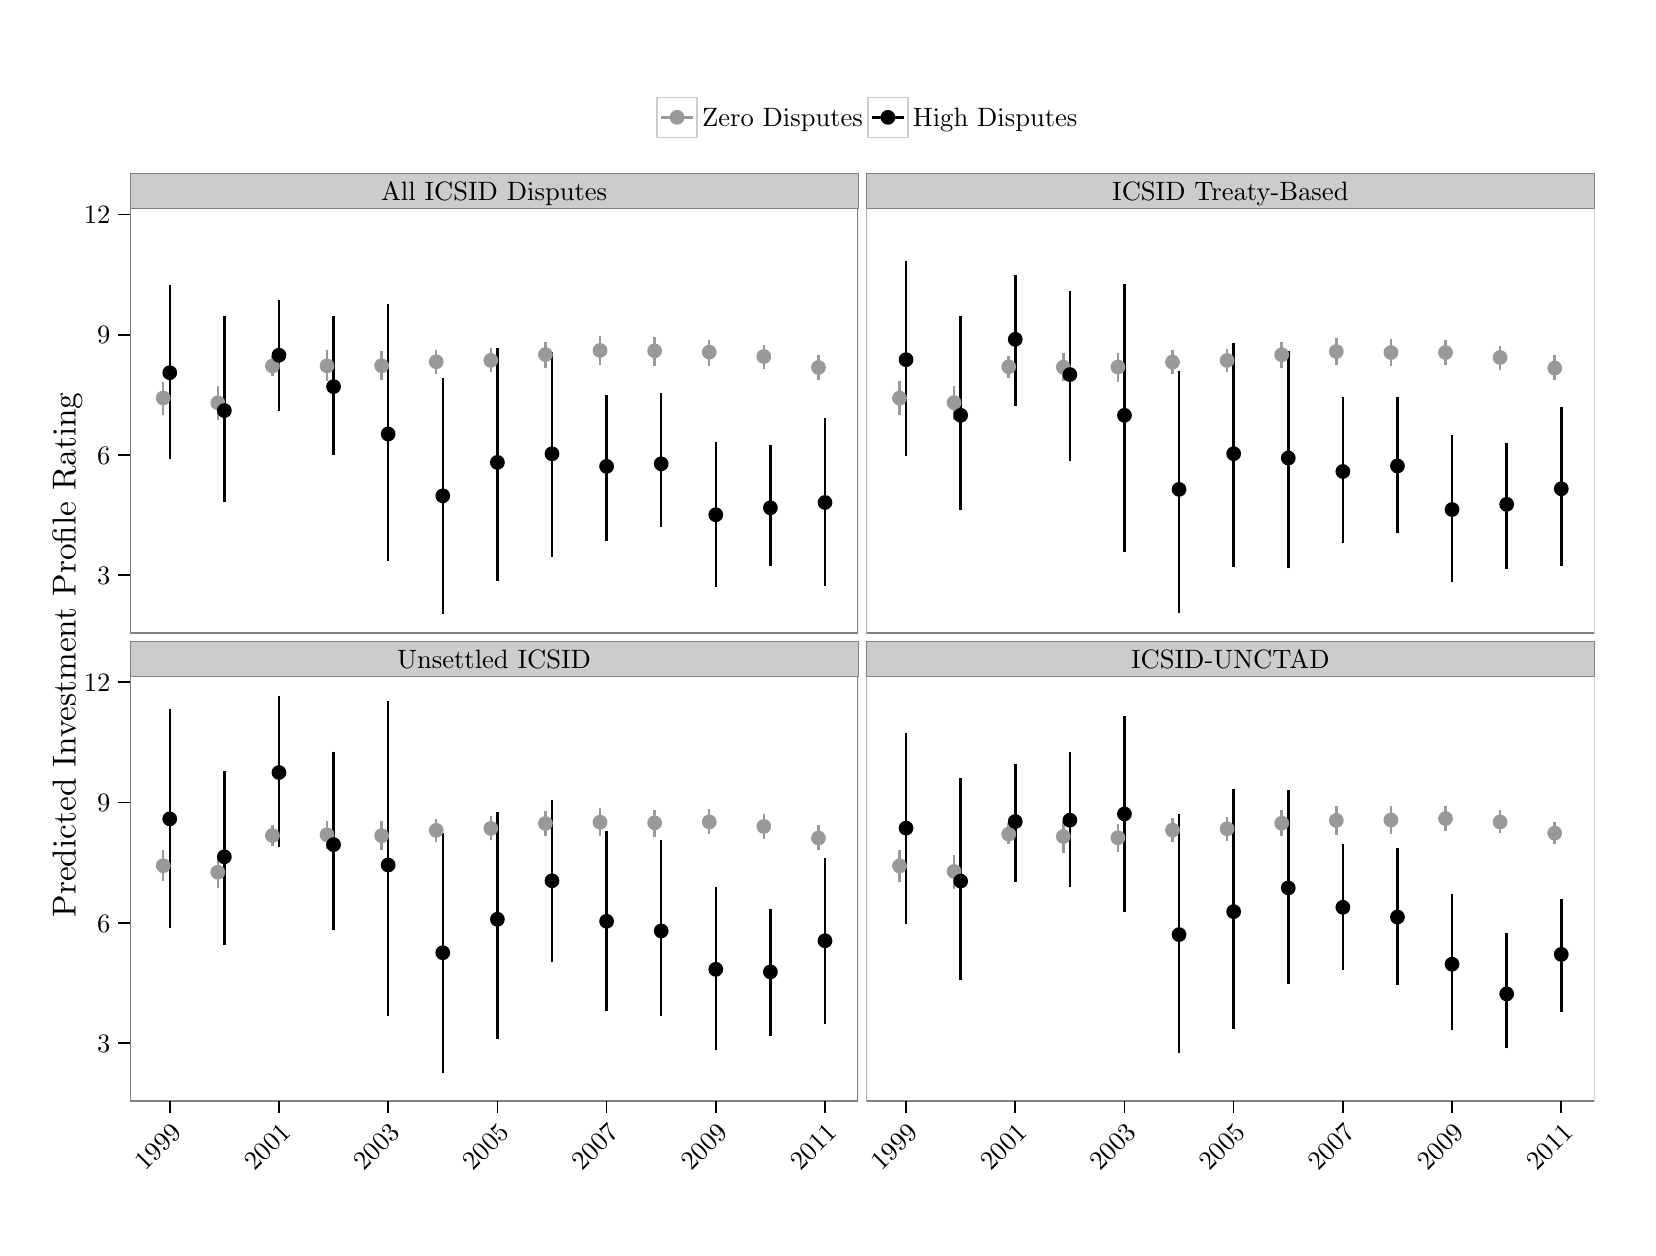
\begin{tikzpicture}[x=1pt,y=1pt]
\definecolor[named]{fillColor}{rgb}{1.00,1.00,1.00}
\path[use as bounding box,fill=fillColor,fill opacity=0.00] (0,0) rectangle (578.16,433.62);
\begin{scope}
\path[clip] (  0.00,  0.00) rectangle (578.16,433.62);
\definecolor[named]{drawColor}{rgb}{1.00,1.00,1.00}
\definecolor[named]{fillColor}{rgb}{1.00,1.00,1.00}

\path[draw=drawColor,line width= 0.6pt,line join=round,line cap=round,fill=fillColor] (  0.00,  0.00) rectangle (578.16,433.62);
\end{scope}
\begin{scope}
\path[clip] ( 37.02,214.77) rectangle (300.06,368.22);
\definecolor[named]{fillColor}{rgb}{1.00,1.00,1.00}

\path[fill=fillColor] ( 37.02,214.77) rectangle (300.06,368.22);
\definecolor[named]{drawColor}{rgb}{0.60,0.60,0.60}
\definecolor[named]{fillColor}{rgb}{0.60,0.60,0.60}

\path[draw=drawColor,line width= 0.9pt,line join=round,fill=fillColor] ( 48.98,293.67) -- ( 48.98,305.59);

\path[draw=drawColor,line width= 0.9pt,line join=round,fill=fillColor] ( 68.71,291.93) -- ( 68.71,304.29);

\path[draw=drawColor,line width= 0.9pt,line join=round,fill=fillColor] ( 88.44,307.70) -- ( 88.44,315.07);

\path[draw=drawColor,line width= 0.9pt,line join=round,fill=fillColor] (108.17,305.93) -- (108.17,317.28);

\path[draw=drawColor,line width= 0.9pt,line join=round,fill=fillColor] (127.90,306.46) -- (127.90,316.72);

\path[draw=drawColor,line width= 0.9pt,line join=round,fill=fillColor] (147.63,308.45) -- (147.63,317.07);

\path[draw=drawColor,line width= 0.9pt,line join=round,fill=fillColor] (167.36,309.24) -- (167.36,317.81);

\path[draw=drawColor,line width= 0.9pt,line join=round,fill=fillColor] (187.09,310.64) -- (187.09,320.16);

\path[draw=drawColor,line width= 0.9pt,line join=round,fill=fillColor] (206.82,311.61) -- (206.82,322.25);

\path[draw=drawColor,line width= 0.9pt,line join=round,fill=fillColor] (226.55,311.45) -- (226.55,321.98);

\path[draw=drawColor,line width= 0.9pt,line join=round,fill=fillColor] (246.28,311.52) -- (246.28,320.82);

\path[draw=drawColor,line width= 0.9pt,line join=round,fill=fillColor] (266.01,310.10) -- (266.01,319.07);

\path[draw=drawColor,line width= 0.9pt,line join=round,fill=fillColor] (285.74,306.38) -- (285.74,315.18);
\definecolor[named]{drawColor}{rgb}{0.00,0.00,0.00}
\definecolor[named]{fillColor}{rgb}{0.00,0.00,0.00}

\path[draw=drawColor,line width= 0.9pt,line join=round,fill=fillColor] ( 51.34,277.65) -- ( 51.34,340.81);

\path[draw=drawColor,line width= 0.9pt,line join=round,fill=fillColor] ( 71.07,262.34) -- ( 71.07,329.49);

\path[draw=drawColor,line width= 0.9pt,line join=round,fill=fillColor] ( 90.80,295.23) -- ( 90.80,335.12);

\path[draw=drawColor,line width= 0.9pt,line join=round,fill=fillColor] (110.53,279.19) -- (110.53,329.36);

\path[draw=drawColor,line width= 0.9pt,line join=round,fill=fillColor] (130.26,240.98) -- (130.26,333.61);

\path[draw=drawColor,line width= 0.9pt,line join=round,fill=fillColor] (150.00,221.74) -- (150.00,307.17);

\path[draw=drawColor,line width= 0.9pt,line join=round,fill=fillColor] (169.73,233.78) -- (169.73,317.86);

\path[draw=drawColor,line width= 0.9pt,line join=round,fill=fillColor] (189.46,242.46) -- (189.46,316.24);

\path[draw=drawColor,line width= 0.9pt,line join=round,fill=fillColor] (209.19,248.30) -- (209.19,300.81);

\path[draw=drawColor,line width= 0.9pt,line join=round,fill=fillColor] (228.92,253.28) -- (228.92,301.49);

\path[draw=drawColor,line width= 0.9pt,line join=round,fill=fillColor] (248.65,231.43) -- (248.65,284.04);

\path[draw=drawColor,line width= 0.9pt,line join=round,fill=fillColor] (268.38,239.20) -- (268.38,282.77);

\path[draw=drawColor,line width= 0.9pt,line join=round,fill=fillColor] (288.11,231.84) -- (288.11,292.68);
\definecolor[named]{fillColor}{rgb}{0.60,0.60,0.60}

\path[fill=fillColor] ( 48.98,299.78) circle (  2.67);
\definecolor[named]{fillColor}{rgb}{0.00,0.00,0.00}

\path[fill=fillColor] ( 51.34,308.94) circle (  2.67);
\definecolor[named]{fillColor}{rgb}{0.60,0.60,0.60}

\path[fill=fillColor] ( 68.71,298.06) circle (  2.67);
\definecolor[named]{fillColor}{rgb}{0.00,0.00,0.00}

\path[fill=fillColor] ( 71.07,295.25) circle (  2.67);
\definecolor[named]{fillColor}{rgb}{0.60,0.60,0.60}

\path[fill=fillColor] ( 88.44,311.37) circle (  2.67);
\definecolor[named]{fillColor}{rgb}{0.00,0.00,0.00}

\path[fill=fillColor] ( 90.80,315.26) circle (  2.67);
\definecolor[named]{fillColor}{rgb}{0.60,0.60,0.60}

\path[fill=fillColor] (108.17,311.43) circle (  2.67);
\definecolor[named]{fillColor}{rgb}{0.00,0.00,0.00}

\path[fill=fillColor] (110.53,303.90) circle (  2.67);
\definecolor[named]{fillColor}{rgb}{0.60,0.60,0.60}

\path[fill=fillColor] (127.90,311.46) circle (  2.67);
\definecolor[named]{fillColor}{rgb}{0.00,0.00,0.00}

\path[fill=fillColor] (130.26,286.79) circle (  2.67);
\definecolor[named]{fillColor}{rgb}{0.60,0.60,0.60}

\path[fill=fillColor] (147.63,312.90) circle (  2.67);
\definecolor[named]{fillColor}{rgb}{0.00,0.00,0.00}

\path[fill=fillColor] (150.00,264.46) circle (  2.67);
\definecolor[named]{fillColor}{rgb}{0.60,0.60,0.60}

\path[fill=fillColor] (167.36,313.40) circle (  2.67);
\definecolor[named]{fillColor}{rgb}{0.00,0.00,0.00}

\path[fill=fillColor] (169.73,276.53) circle (  2.67);
\definecolor[named]{fillColor}{rgb}{0.60,0.60,0.60}

\path[fill=fillColor] (187.09,315.49) circle (  2.67);
\definecolor[named]{fillColor}{rgb}{0.00,0.00,0.00}

\path[fill=fillColor] (189.46,279.64) circle (  2.67);
\definecolor[named]{fillColor}{rgb}{0.60,0.60,0.60}

\path[fill=fillColor] (206.82,316.99) circle (  2.67);
\definecolor[named]{fillColor}{rgb}{0.00,0.00,0.00}

\path[fill=fillColor] (209.19,275.10) circle (  2.67);
\definecolor[named]{fillColor}{rgb}{0.60,0.60,0.60}

\path[fill=fillColor] (226.55,316.84) circle (  2.67);
\definecolor[named]{fillColor}{rgb}{0.00,0.00,0.00}

\path[fill=fillColor] (228.92,276.03) circle (  2.67);
\definecolor[named]{fillColor}{rgb}{0.60,0.60,0.60}

\path[fill=fillColor] (246.28,316.38) circle (  2.67);
\definecolor[named]{fillColor}{rgb}{0.00,0.00,0.00}

\path[fill=fillColor] (248.65,257.61) circle (  2.67);
\definecolor[named]{fillColor}{rgb}{0.60,0.60,0.60}

\path[fill=fillColor] (266.01,314.79) circle (  2.67);
\definecolor[named]{fillColor}{rgb}{0.00,0.00,0.00}

\path[fill=fillColor] (268.38,260.12) circle (  2.67);
\definecolor[named]{fillColor}{rgb}{0.60,0.60,0.60}

\path[fill=fillColor] (285.74,310.83) circle (  2.67);
\definecolor[named]{fillColor}{rgb}{0.00,0.00,0.00}

\path[fill=fillColor] (288.11,262.05) circle (  2.67);
\definecolor[named]{drawColor}{rgb}{0.50,0.50,0.50}

\path[draw=drawColor,line width= 0.6pt,line join=round,line cap=round] ( 37.02,214.77) rectangle (300.06,368.22);
\end{scope}
\begin{scope}
\path[clip] (303.07,214.77) rectangle (566.12,368.22);
\definecolor[named]{fillColor}{rgb}{1.00,1.00,1.00}

\path[fill=fillColor] (303.07,214.77) rectangle (566.12,368.22);
\definecolor[named]{drawColor}{rgb}{0.60,0.60,0.60}
\definecolor[named]{fillColor}{rgb}{0.60,0.60,0.60}

\path[draw=drawColor,line width= 0.9pt,line join=round,fill=fillColor] (315.03,293.78) -- (315.03,305.84);

\path[draw=drawColor,line width= 0.9pt,line join=round,fill=fillColor] (334.76,291.95) -- (334.76,304.13);

\path[draw=drawColor,line width= 0.9pt,line join=round,fill=fillColor] (354.49,307.16) -- (354.49,314.84);

\path[draw=drawColor,line width= 0.9pt,line join=round,fill=fillColor] (374.22,305.98) -- (374.22,316.10);

\path[draw=drawColor,line width= 0.9pt,line join=round,fill=fillColor] (393.95,305.73) -- (393.95,316.18);

\path[draw=drawColor,line width= 0.9pt,line join=round,fill=fillColor] (413.68,308.47) -- (413.68,316.99);

\path[draw=drawColor,line width= 0.9pt,line join=round,fill=fillColor] (433.41,309.08) -- (433.41,317.58);

\path[draw=drawColor,line width= 0.9pt,line join=round,fill=fillColor] (453.14,310.77) -- (453.14,319.96);

\path[draw=drawColor,line width= 0.9pt,line join=round,fill=fillColor] (472.87,311.76) -- (472.87,321.65);

\path[draw=drawColor,line width= 0.9pt,line join=round,fill=fillColor] (492.60,311.49) -- (492.60,321.25);

\path[draw=drawColor,line width= 0.9pt,line join=round,fill=fillColor] (512.33,311.80) -- (512.33,320.87);

\path[draw=drawColor,line width= 0.9pt,line join=round,fill=fillColor] (532.06,310.00) -- (532.06,318.75);

\path[draw=drawColor,line width= 0.9pt,line join=round,fill=fillColor] (551.79,306.27) -- (551.79,315.18);
\definecolor[named]{drawColor}{rgb}{0.00,0.00,0.00}
\definecolor[named]{fillColor}{rgb}{0.00,0.00,0.00}

\path[draw=drawColor,line width= 0.9pt,line join=round,fill=fillColor] (317.40,278.99) -- (317.40,349.30);

\path[draw=drawColor,line width= 0.9pt,line join=round,fill=fillColor] (337.13,259.18) -- (337.13,329.45);

\path[draw=drawColor,line width= 0.9pt,line join=round,fill=fillColor] (356.86,296.83) -- (356.86,344.32);

\path[draw=drawColor,line width= 0.9pt,line join=round,fill=fillColor] (376.59,276.90) -- (376.59,338.49);

\path[draw=drawColor,line width= 0.9pt,line join=round,fill=fillColor] (396.32,243.99) -- (396.32,340.82);

\path[draw=drawColor,line width= 0.9pt,line join=round,fill=fillColor] (416.05,221.97) -- (416.05,309.69);

\path[draw=drawColor,line width= 0.9pt,line join=round,fill=fillColor] (435.78,238.83) -- (435.78,319.61);

\path[draw=drawColor,line width= 0.9pt,line join=round,fill=fillColor] (455.51,238.22) -- (455.51,316.91);

\path[draw=drawColor,line width= 0.9pt,line join=round,fill=fillColor] (475.24,247.41) -- (475.24,300.28);

\path[draw=drawColor,line width= 0.9pt,line join=round,fill=fillColor] (494.97,251.06) -- (494.97,300.07);

\path[draw=drawColor,line width= 0.9pt,line join=round,fill=fillColor] (514.70,233.31) -- (514.70,286.29);

\path[draw=drawColor,line width= 0.9pt,line join=round,fill=fillColor] (534.43,238.00) -- (534.43,283.55);

\path[draw=drawColor,line width= 0.9pt,line join=round,fill=fillColor] (554.16,238.96) -- (554.16,296.55);
\definecolor[named]{fillColor}{rgb}{0.60,0.60,0.60}

\path[fill=fillColor] (315.03,299.76) circle (  2.67);
\definecolor[named]{fillColor}{rgb}{0.00,0.00,0.00}

\path[fill=fillColor] (317.40,313.65) circle (  2.67);
\definecolor[named]{fillColor}{rgb}{0.60,0.60,0.60}

\path[fill=fillColor] (334.76,298.12) circle (  2.67);
\definecolor[named]{fillColor}{rgb}{0.00,0.00,0.00}

\path[fill=fillColor] (337.13,293.55) circle (  2.67);
\definecolor[named]{fillColor}{rgb}{0.60,0.60,0.60}

\path[fill=fillColor] (354.49,311.08) circle (  2.67);
\definecolor[named]{fillColor}{rgb}{0.00,0.00,0.00}

\path[fill=fillColor] (356.86,321.00) circle (  2.67);
\definecolor[named]{fillColor}{rgb}{0.60,0.60,0.60}

\path[fill=fillColor] (374.22,310.94) circle (  2.67);
\definecolor[named]{fillColor}{rgb}{0.00,0.00,0.00}

\path[fill=fillColor] (376.59,308.26) circle (  2.67);
\definecolor[named]{fillColor}{rgb}{0.60,0.60,0.60}

\path[fill=fillColor] (393.95,310.98) circle (  2.67);
\definecolor[named]{fillColor}{rgb}{0.00,0.00,0.00}

\path[fill=fillColor] (396.32,293.54) circle (  2.67);
\definecolor[named]{fillColor}{rgb}{0.60,0.60,0.60}

\path[fill=fillColor] (413.68,312.77) circle (  2.67);
\definecolor[named]{fillColor}{rgb}{0.00,0.00,0.00}

\path[fill=fillColor] (416.05,266.78) circle (  2.67);
\definecolor[named]{fillColor}{rgb}{0.60,0.60,0.60}

\path[fill=fillColor] (433.41,313.37) circle (  2.67);
\definecolor[named]{fillColor}{rgb}{0.00,0.00,0.00}

\path[fill=fillColor] (435.78,279.67) circle (  2.67);
\definecolor[named]{fillColor}{rgb}{0.60,0.60,0.60}

\path[fill=fillColor] (453.14,315.42) circle (  2.67);
\definecolor[named]{fillColor}{rgb}{0.00,0.00,0.00}

\path[fill=fillColor] (455.51,278.10) circle (  2.67);
\definecolor[named]{fillColor}{rgb}{0.60,0.60,0.60}

\path[fill=fillColor] (472.87,316.62) circle (  2.67);
\definecolor[named]{fillColor}{rgb}{0.00,0.00,0.00}

\path[fill=fillColor] (475.24,273.25) circle (  2.67);
\definecolor[named]{fillColor}{rgb}{0.60,0.60,0.60}

\path[fill=fillColor] (492.60,316.22) circle (  2.67);
\definecolor[named]{fillColor}{rgb}{0.00,0.00,0.00}

\path[fill=fillColor] (494.97,275.25) circle (  2.67);
\definecolor[named]{fillColor}{rgb}{0.60,0.60,0.60}

\path[fill=fillColor] (512.33,316.24) circle (  2.67);
\definecolor[named]{fillColor}{rgb}{0.00,0.00,0.00}

\path[fill=fillColor] (514.70,259.49) circle (  2.67);
\definecolor[named]{fillColor}{rgb}{0.60,0.60,0.60}

\path[fill=fillColor] (532.06,314.44) circle (  2.67);
\definecolor[named]{fillColor}{rgb}{0.00,0.00,0.00}

\path[fill=fillColor] (534.43,261.38) circle (  2.67);
\definecolor[named]{fillColor}{rgb}{0.60,0.60,0.60}

\path[fill=fillColor] (551.79,310.60) circle (  2.67);
\definecolor[named]{fillColor}{rgb}{0.00,0.00,0.00}

\path[fill=fillColor] (554.16,266.99) circle (  2.67);
\definecolor[named]{drawColor}{rgb}{0.50,0.50,0.50}

\path[draw=drawColor,line width= 0.6pt,line join=round,line cap=round] (303.07,214.77) rectangle (566.12,368.22);
\end{scope}
\begin{scope}
\path[clip] ( 37.02, 45.67) rectangle (300.06,199.12);
\definecolor[named]{fillColor}{rgb}{1.00,1.00,1.00}

\path[fill=fillColor] ( 37.02, 45.67) rectangle (300.06,199.12);
\definecolor[named]{drawColor}{rgb}{0.60,0.60,0.60}
\definecolor[named]{fillColor}{rgb}{0.60,0.60,0.60}

\path[draw=drawColor,line width= 0.9pt,line join=round,fill=fillColor] ( 48.98,125.38) -- ( 48.98,136.64);

\path[draw=drawColor,line width= 0.9pt,line join=round,fill=fillColor] ( 68.71,122.62) -- ( 68.71,134.68);

\path[draw=drawColor,line width= 0.9pt,line join=round,fill=fillColor] ( 88.44,137.99) -- ( 88.44,145.38);

\path[draw=drawColor,line width= 0.9pt,line join=round,fill=fillColor] (108.17,136.92) -- (108.17,146.80);

\path[draw=drawColor,line width= 0.9pt,line join=round,fill=fillColor] (127.90,136.43) -- (127.90,146.97);

\path[draw=drawColor,line width= 0.9pt,line join=round,fill=fillColor] (147.63,139.21) -- (147.63,147.84);

\path[draw=drawColor,line width= 0.9pt,line join=round,fill=fillColor] (167.36,139.98) -- (167.36,148.92);

\path[draw=drawColor,line width= 0.9pt,line join=round,fill=fillColor] (187.09,141.35) -- (187.09,150.56);

\path[draw=drawColor,line width= 0.9pt,line join=round,fill=fillColor] (206.82,141.52) -- (206.82,151.53);

\path[draw=drawColor,line width= 0.9pt,line join=round,fill=fillColor] (226.55,141.08) -- (226.55,151.10);

\path[draw=drawColor,line width= 0.9pt,line join=round,fill=fillColor] (246.28,142.10) -- (246.28,151.31);

\path[draw=drawColor,line width= 0.9pt,line join=round,fill=fillColor] (266.01,140.56) -- (266.01,149.61);

\path[draw=drawColor,line width= 0.9pt,line join=round,fill=fillColor] (285.74,136.44) -- (285.74,145.36);
\definecolor[named]{drawColor}{rgb}{0.00,0.00,0.00}
\definecolor[named]{fillColor}{rgb}{0.00,0.00,0.00}

\path[draw=drawColor,line width= 0.9pt,line join=round,fill=fillColor] ( 51.34,108.37) -- ( 51.34,187.25);

\path[draw=drawColor,line width= 0.9pt,line join=round,fill=fillColor] ( 71.07,102.13) -- ( 71.07,165.18);

\path[draw=drawColor,line width= 0.9pt,line join=round,fill=fillColor] ( 90.80,137.47) -- ( 90.80,192.15);

\path[draw=drawColor,line width= 0.9pt,line join=round,fill=fillColor] (110.53,107.39) -- (110.53,171.99);

\path[draw=drawColor,line width= 0.9pt,line join=round,fill=fillColor] (130.26, 76.50) -- (130.26,190.14);

\path[draw=drawColor,line width= 0.9pt,line join=round,fill=fillColor] (150.00, 55.81) -- (150.00,142.68);

\path[draw=drawColor,line width= 0.9pt,line join=round,fill=fillColor] (169.73, 68.20) -- (169.73,150.27);

\path[draw=drawColor,line width= 0.9pt,line join=round,fill=fillColor] (189.46, 95.95) -- (189.46,154.62);

\path[draw=drawColor,line width= 0.9pt,line join=round,fill=fillColor] (209.19, 78.21) -- (209.19,143.42);

\path[draw=drawColor,line width= 0.9pt,line join=round,fill=fillColor] (228.92, 76.53) -- (228.92,140.01);

\path[draw=drawColor,line width= 0.9pt,line join=round,fill=fillColor] (248.65, 64.08) -- (248.65,123.27);

\path[draw=drawColor,line width= 0.9pt,line join=round,fill=fillColor] (268.38, 69.38) -- (268.38,115.03);

\path[draw=drawColor,line width= 0.9pt,line join=round,fill=fillColor] (288.11, 73.63) -- (288.11,133.71);
\definecolor[named]{fillColor}{rgb}{0.60,0.60,0.60}

\path[fill=fillColor] ( 48.98,130.79) circle (  2.67);
\definecolor[named]{fillColor}{rgb}{0.00,0.00,0.00}

\path[fill=fillColor] ( 51.34,147.73) circle (  2.67);
\definecolor[named]{fillColor}{rgb}{0.60,0.60,0.60}

\path[fill=fillColor] ( 68.71,128.45) circle (  2.67);
\definecolor[named]{fillColor}{rgb}{0.00,0.00,0.00}

\path[fill=fillColor] ( 71.07,134.01) circle (  2.67);
\definecolor[named]{fillColor}{rgb}{0.60,0.60,0.60}

\path[fill=fillColor] ( 88.44,141.70) circle (  2.67);
\definecolor[named]{fillColor}{rgb}{0.00,0.00,0.00}

\path[fill=fillColor] ( 90.80,164.47) circle (  2.67);
\definecolor[named]{fillColor}{rgb}{0.60,0.60,0.60}

\path[fill=fillColor] (108.17,141.95) circle (  2.67);
\definecolor[named]{fillColor}{rgb}{0.00,0.00,0.00}

\path[fill=fillColor] (110.53,138.41) circle (  2.67);
\definecolor[named]{fillColor}{rgb}{0.60,0.60,0.60}

\path[fill=fillColor] (127.90,141.65) circle (  2.67);
\definecolor[named]{fillColor}{rgb}{0.00,0.00,0.00}

\path[fill=fillColor] (130.26,131.04) circle (  2.67);
\definecolor[named]{fillColor}{rgb}{0.60,0.60,0.60}

\path[fill=fillColor] (147.63,143.57) circle (  2.67);
\definecolor[named]{fillColor}{rgb}{0.00,0.00,0.00}

\path[fill=fillColor] (150.00, 99.35) circle (  2.67);
\definecolor[named]{fillColor}{rgb}{0.60,0.60,0.60}

\path[fill=fillColor] (167.36,144.27) circle (  2.67);
\definecolor[named]{fillColor}{rgb}{0.00,0.00,0.00}

\path[fill=fillColor] (169.73,111.43) circle (  2.67);
\definecolor[named]{fillColor}{rgb}{0.60,0.60,0.60}

\path[fill=fillColor] (187.09,146.06) circle (  2.67);
\definecolor[named]{fillColor}{rgb}{0.00,0.00,0.00}

\path[fill=fillColor] (189.46,125.36) circle (  2.67);
\definecolor[named]{fillColor}{rgb}{0.60,0.60,0.60}

\path[fill=fillColor] (206.82,146.52) circle (  2.67);
\definecolor[named]{fillColor}{rgb}{0.00,0.00,0.00}

\path[fill=fillColor] (209.19,110.72) circle (  2.67);
\definecolor[named]{fillColor}{rgb}{0.60,0.60,0.60}

\path[fill=fillColor] (226.55,146.28) circle (  2.67);
\definecolor[named]{fillColor}{rgb}{0.00,0.00,0.00}

\path[fill=fillColor] (228.92,107.22) circle (  2.67);
\definecolor[named]{fillColor}{rgb}{0.60,0.60,0.60}

\path[fill=fillColor] (246.28,146.63) circle (  2.67);
\definecolor[named]{fillColor}{rgb}{0.00,0.00,0.00}

\path[fill=fillColor] (248.65, 93.35) circle (  2.67);
\definecolor[named]{fillColor}{rgb}{0.60,0.60,0.60}

\path[fill=fillColor] (266.01,144.98) circle (  2.67);
\definecolor[named]{fillColor}{rgb}{0.00,0.00,0.00}

\path[fill=fillColor] (268.38, 92.43) circle (  2.67);
\definecolor[named]{fillColor}{rgb}{0.60,0.60,0.60}

\path[fill=fillColor] (285.74,140.79) circle (  2.67);
\definecolor[named]{fillColor}{rgb}{0.00,0.00,0.00}

\path[fill=fillColor] (288.11,103.67) circle (  2.67);
\definecolor[named]{drawColor}{rgb}{0.50,0.50,0.50}

\path[draw=drawColor,line width= 0.6pt,line join=round,line cap=round] ( 37.02, 45.67) rectangle (300.06,199.12);
\end{scope}
\begin{scope}
\path[clip] (303.07, 45.67) rectangle (566.12,199.12);
\definecolor[named]{fillColor}{rgb}{1.00,1.00,1.00}

\path[fill=fillColor] (303.07, 45.67) rectangle (566.12,199.12);
\definecolor[named]{drawColor}{rgb}{0.60,0.60,0.60}
\definecolor[named]{fillColor}{rgb}{0.60,0.60,0.60}

\path[draw=drawColor,line width= 0.9pt,line join=round,fill=fillColor] (315.03,124.77) -- (315.03,136.40);

\path[draw=drawColor,line width= 0.9pt,line join=round,fill=fillColor] (334.76,122.55) -- (334.76,134.49);

\path[draw=drawColor,line width= 0.9pt,line join=round,fill=fillColor] (354.49,138.58) -- (354.49,146.09);

\path[draw=drawColor,line width= 0.9pt,line join=round,fill=fillColor] (374.22,135.46) -- (374.22,146.59);

\path[draw=drawColor,line width= 0.9pt,line join=round,fill=fillColor] (393.95,135.88) -- (393.95,145.95);

\path[draw=drawColor,line width= 0.9pt,line join=round,fill=fillColor] (413.68,139.39) -- (413.68,147.97);

\path[draw=drawColor,line width= 0.9pt,line join=round,fill=fillColor] (433.41,139.78) -- (433.41,148.45);

\path[draw=drawColor,line width= 0.9pt,line join=round,fill=fillColor] (453.14,141.53) -- (453.14,150.88);

\path[draw=drawColor,line width= 0.9pt,line join=round,fill=fillColor] (472.87,141.91) -- (472.87,152.29);

\path[draw=drawColor,line width= 0.9pt,line join=round,fill=fillColor] (492.60,142.20) -- (492.60,152.36);

\path[draw=drawColor,line width= 0.9pt,line join=round,fill=fillColor] (512.33,143.35) -- (512.33,152.28);

\path[draw=drawColor,line width= 0.9pt,line join=round,fill=fillColor] (532.06,142.45) -- (532.06,150.85);

\path[draw=drawColor,line width= 0.9pt,line join=round,fill=fillColor] (551.79,138.48) -- (551.79,146.68);
\definecolor[named]{drawColor}{rgb}{0.00,0.00,0.00}
\definecolor[named]{fillColor}{rgb}{0.00,0.00,0.00}

\path[draw=drawColor,line width= 0.9pt,line join=round,fill=fillColor] (317.40,109.70) -- (317.40,178.73);

\path[draw=drawColor,line width= 0.9pt,line join=round,fill=fillColor] (337.13, 89.60) -- (337.13,162.56);

\path[draw=drawColor,line width= 0.9pt,line join=round,fill=fillColor] (356.86,124.91) -- (356.86,167.47);

\path[draw=drawColor,line width= 0.9pt,line join=round,fill=fillColor] (376.59,122.92) -- (376.59,171.79);

\path[draw=drawColor,line width= 0.9pt,line join=round,fill=fillColor] (396.32,113.96) -- (396.32,184.97);

\path[draw=drawColor,line width= 0.9pt,line join=round,fill=fillColor] (416.05, 62.98) -- (416.05,149.42);

\path[draw=drawColor,line width= 0.9pt,line join=round,fill=fillColor] (435.78, 71.72) -- (435.78,158.52);

\path[draw=drawColor,line width= 0.9pt,line join=round,fill=fillColor] (455.51, 88.23) -- (455.51,158.15);

\path[draw=drawColor,line width= 0.9pt,line join=round,fill=fillColor] (475.24, 93.25) -- (475.24,138.81);

\path[draw=drawColor,line width= 0.9pt,line join=round,fill=fillColor] (494.97, 87.78) -- (494.97,137.21);

\path[draw=drawColor,line width= 0.9pt,line join=round,fill=fillColor] (514.70, 71.48) -- (514.70,120.63);

\path[draw=drawColor,line width= 0.9pt,line join=round,fill=fillColor] (534.43, 64.78) -- (534.43,106.32);

\path[draw=drawColor,line width= 0.9pt,line join=round,fill=fillColor] (554.16, 77.99) -- (554.16,118.94);
\definecolor[named]{fillColor}{rgb}{0.60,0.60,0.60}

\path[fill=fillColor] (315.03,130.70) circle (  2.67);
\definecolor[named]{fillColor}{rgb}{0.00,0.00,0.00}

\path[fill=fillColor] (317.40,144.37) circle (  2.67);
\definecolor[named]{fillColor}{rgb}{0.60,0.60,0.60}

\path[fill=fillColor] (334.76,128.73) circle (  2.67);
\definecolor[named]{fillColor}{rgb}{0.00,0.00,0.00}

\path[fill=fillColor] (337.13,125.24) circle (  2.67);
\definecolor[named]{fillColor}{rgb}{0.60,0.60,0.60}

\path[fill=fillColor] (354.49,142.20) circle (  2.67);
\definecolor[named]{fillColor}{rgb}{0.00,0.00,0.00}

\path[fill=fillColor] (356.86,146.75) circle (  2.67);
\definecolor[named]{fillColor}{rgb}{0.60,0.60,0.60}

\path[fill=fillColor] (374.22,141.34) circle (  2.67);
\definecolor[named]{fillColor}{rgb}{0.00,0.00,0.00}

\path[fill=fillColor] (376.59,147.24) circle (  2.67);
\definecolor[named]{fillColor}{rgb}{0.60,0.60,0.60}

\path[fill=fillColor] (393.95,140.90) circle (  2.67);
\definecolor[named]{fillColor}{rgb}{0.00,0.00,0.00}

\path[fill=fillColor] (396.32,149.51) circle (  2.67);
\definecolor[named]{fillColor}{rgb}{0.60,0.60,0.60}

\path[fill=fillColor] (413.68,143.66) circle (  2.67);
\definecolor[named]{fillColor}{rgb}{0.00,0.00,0.00}

\path[fill=fillColor] (416.05,105.90) circle (  2.67);
\definecolor[named]{fillColor}{rgb}{0.60,0.60,0.60}

\path[fill=fillColor] (433.41,144.13) circle (  2.67);
\definecolor[named]{fillColor}{rgb}{0.00,0.00,0.00}

\path[fill=fillColor] (435.78,114.21) circle (  2.67);
\definecolor[named]{fillColor}{rgb}{0.60,0.60,0.60}

\path[fill=fillColor] (453.14,146.15) circle (  2.67);
\definecolor[named]{fillColor}{rgb}{0.00,0.00,0.00}

\path[fill=fillColor] (455.51,122.77) circle (  2.67);
\definecolor[named]{fillColor}{rgb}{0.60,0.60,0.60}

\path[fill=fillColor] (472.87,147.15) circle (  2.67);
\definecolor[named]{fillColor}{rgb}{0.00,0.00,0.00}

\path[fill=fillColor] (475.24,115.76) circle (  2.67);
\definecolor[named]{fillColor}{rgb}{0.60,0.60,0.60}

\path[fill=fillColor] (492.60,147.30) circle (  2.67);
\definecolor[named]{fillColor}{rgb}{0.00,0.00,0.00}

\path[fill=fillColor] (494.97,112.25) circle (  2.67);
\definecolor[named]{fillColor}{rgb}{0.60,0.60,0.60}

\path[fill=fillColor] (512.33,147.83) circle (  2.67);
\definecolor[named]{fillColor}{rgb}{0.00,0.00,0.00}

\path[fill=fillColor] (514.70, 95.21) circle (  2.67);
\definecolor[named]{fillColor}{rgb}{0.60,0.60,0.60}

\path[fill=fillColor] (532.06,146.59) circle (  2.67);
\definecolor[named]{fillColor}{rgb}{0.00,0.00,0.00}

\path[fill=fillColor] (534.43, 84.49) circle (  2.67);
\definecolor[named]{fillColor}{rgb}{0.60,0.60,0.60}

\path[fill=fillColor] (551.79,142.58) circle (  2.67);
\definecolor[named]{fillColor}{rgb}{0.00,0.00,0.00}

\path[fill=fillColor] (554.16, 98.75) circle (  2.67);
\definecolor[named]{drawColor}{rgb}{0.50,0.50,0.50}

\path[draw=drawColor,line width= 0.6pt,line join=round,line cap=round] (303.07, 45.67) rectangle (566.12,199.12);
\end{scope}
\begin{scope}
\path[clip] (  0.00,  0.00) rectangle (578.16,433.62);
\definecolor[named]{drawColor}{rgb}{0.50,0.50,0.50}
\definecolor[named]{fillColor}{rgb}{0.80,0.80,0.80}

\path[draw=drawColor,line width= 0.2pt,line join=round,line cap=round,fill=fillColor] ( 37.02,368.22) rectangle (300.06,380.85);
\definecolor[named]{drawColor}{rgb}{0.00,0.00,0.00}

\node[text=drawColor,anchor=base,inner sep=0pt, outer sep=0pt, scale=  0.96] at (168.54,371.23) {All ICSID Disputes};
\end{scope}
\begin{scope}
\path[clip] (  0.00,  0.00) rectangle (578.16,433.62);
\definecolor[named]{drawColor}{rgb}{0.50,0.50,0.50}
\definecolor[named]{fillColor}{rgb}{0.80,0.80,0.80}

\path[draw=drawColor,line width= 0.2pt,line join=round,line cap=round,fill=fillColor] (303.07,368.22) rectangle (566.12,380.85);
\definecolor[named]{drawColor}{rgb}{0.00,0.00,0.00}

\node[text=drawColor,anchor=base,inner sep=0pt, outer sep=0pt, scale=  0.96] at (434.59,371.23) {ICSID Treaty-Based};
\end{scope}
\begin{scope}
\path[clip] (  0.00,  0.00) rectangle (578.16,433.62);
\definecolor[named]{drawColor}{rgb}{0.50,0.50,0.50}
\definecolor[named]{fillColor}{rgb}{0.80,0.80,0.80}

\path[draw=drawColor,line width= 0.2pt,line join=round,line cap=round,fill=fillColor] ( 37.02,199.12) rectangle (300.06,211.75);
\definecolor[named]{drawColor}{rgb}{0.00,0.00,0.00}

\node[text=drawColor,anchor=base,inner sep=0pt, outer sep=0pt, scale=  0.96] at (168.54,202.13) {Unsettled ICSID};
\end{scope}
\begin{scope}
\path[clip] (  0.00,  0.00) rectangle (578.16,433.62);
\definecolor[named]{drawColor}{rgb}{0.50,0.50,0.50}
\definecolor[named]{fillColor}{rgb}{0.80,0.80,0.80}

\path[draw=drawColor,line width= 0.2pt,line join=round,line cap=round,fill=fillColor] (303.07,199.12) rectangle (566.12,211.75);
\definecolor[named]{drawColor}{rgb}{0.00,0.00,0.00}

\node[text=drawColor,anchor=base,inner sep=0pt, outer sep=0pt, scale=  0.96] at (434.59,202.13) {ICSID-UNCTAD};
\end{scope}
\begin{scope}
\path[clip] (  0.00,  0.00) rectangle (578.16,433.62);
\definecolor[named]{drawColor}{rgb}{0.00,0.00,0.00}

\node[text=drawColor,anchor=base east,inner sep=0pt, outer sep=0pt, scale=  0.96] at ( 29.91,232.42) {3};

\node[text=drawColor,anchor=base east,inner sep=0pt, outer sep=0pt, scale=  0.96] at ( 29.91,275.90) {6};

\node[text=drawColor,anchor=base east,inner sep=0pt, outer sep=0pt, scale=  0.96] at ( 29.91,319.38) {9};

\node[text=drawColor,anchor=base east,inner sep=0pt, outer sep=0pt, scale=  0.96] at ( 29.91,362.86) {12};
\end{scope}
\begin{scope}
\path[clip] (  0.00,  0.00) rectangle (578.16,433.62);
\definecolor[named]{drawColor}{rgb}{0.00,0.00,0.00}

\path[draw=drawColor,line width= 0.6pt,line join=round] ( 32.75,235.73) --
	( 37.02,235.73);

\path[draw=drawColor,line width= 0.6pt,line join=round] ( 32.75,279.21) --
	( 37.02,279.21);

\path[draw=drawColor,line width= 0.6pt,line join=round] ( 32.75,322.68) --
	( 37.02,322.68);

\path[draw=drawColor,line width= 0.6pt,line join=round] ( 32.75,366.16) --
	( 37.02,366.16);
\end{scope}
\begin{scope}
\path[clip] (  0.00,  0.00) rectangle (578.16,433.62);
\definecolor[named]{drawColor}{rgb}{0.00,0.00,0.00}

\node[text=drawColor,anchor=base east,inner sep=0pt, outer sep=0pt, scale=  0.96] at ( 29.91, 63.33) {3};

\node[text=drawColor,anchor=base east,inner sep=0pt, outer sep=0pt, scale=  0.96] at ( 29.91,106.81) {6};

\node[text=drawColor,anchor=base east,inner sep=0pt, outer sep=0pt, scale=  0.96] at ( 29.91,150.28) {9};

\node[text=drawColor,anchor=base east,inner sep=0pt, outer sep=0pt, scale=  0.96] at ( 29.91,193.76) {12};
\end{scope}
\begin{scope}
\path[clip] (  0.00,  0.00) rectangle (578.16,433.62);
\definecolor[named]{drawColor}{rgb}{0.00,0.00,0.00}

\path[draw=drawColor,line width= 0.6pt,line join=round] ( 32.75, 66.63) --
	( 37.02, 66.63);

\path[draw=drawColor,line width= 0.6pt,line join=round] ( 32.75,110.11) --
	( 37.02,110.11);

\path[draw=drawColor,line width= 0.6pt,line join=round] ( 32.75,153.59) --
	( 37.02,153.59);

\path[draw=drawColor,line width= 0.6pt,line join=round] ( 32.75,197.07) --
	( 37.02,197.07);
\end{scope}
\begin{scope}
\path[clip] (  0.00,  0.00) rectangle (578.16,433.62);
\definecolor[named]{drawColor}{rgb}{0.00,0.00,0.00}

\path[draw=drawColor,line width= 0.6pt,line join=round] ( 51.34, 41.40) --
	( 51.34, 45.67);

\path[draw=drawColor,line width= 0.6pt,line join=round] ( 90.80, 41.40) --
	( 90.80, 45.67);

\path[draw=drawColor,line width= 0.6pt,line join=round] (130.26, 41.40) --
	(130.26, 45.67);

\path[draw=drawColor,line width= 0.6pt,line join=round] (169.73, 41.40) --
	(169.73, 45.67);

\path[draw=drawColor,line width= 0.6pt,line join=round] (209.19, 41.40) --
	(209.19, 45.67);

\path[draw=drawColor,line width= 0.6pt,line join=round] (248.65, 41.40) --
	(248.65, 45.67);

\path[draw=drawColor,line width= 0.6pt,line join=round] (288.11, 41.40) --
	(288.11, 45.67);
\end{scope}
\begin{scope}
\path[clip] (  0.00,  0.00) rectangle (578.16,433.62);
\definecolor[named]{drawColor}{rgb}{0.00,0.00,0.00}

\node[text=drawColor,rotate= 45.00,anchor=base east,inner sep=0pt, outer sep=0pt, scale=  0.96] at ( 56.02, 33.88) {1999};

\node[text=drawColor,rotate= 45.00,anchor=base east,inner sep=0pt, outer sep=0pt, scale=  0.96] at ( 95.48, 33.88) {2001};

\node[text=drawColor,rotate= 45.00,anchor=base east,inner sep=0pt, outer sep=0pt, scale=  0.96] at (134.94, 33.88) {2003};

\node[text=drawColor,rotate= 45.00,anchor=base east,inner sep=0pt, outer sep=0pt, scale=  0.96] at (174.40, 33.88) {2005};

\node[text=drawColor,rotate= 45.00,anchor=base east,inner sep=0pt, outer sep=0pt, scale=  0.96] at (213.86, 33.88) {2007};

\node[text=drawColor,rotate= 45.00,anchor=base east,inner sep=0pt, outer sep=0pt, scale=  0.96] at (253.32, 33.88) {2009};

\node[text=drawColor,rotate= 45.00,anchor=base east,inner sep=0pt, outer sep=0pt, scale=  0.96] at (292.78, 33.88) {2011};
\end{scope}
\begin{scope}
\path[clip] (  0.00,  0.00) rectangle (578.16,433.62);
\definecolor[named]{drawColor}{rgb}{0.00,0.00,0.00}

\path[draw=drawColor,line width= 0.6pt,line join=round] (317.40, 41.40) --
	(317.40, 45.67);

\path[draw=drawColor,line width= 0.6pt,line join=round] (356.86, 41.40) --
	(356.86, 45.67);

\path[draw=drawColor,line width= 0.6pt,line join=round] (396.32, 41.40) --
	(396.32, 45.67);

\path[draw=drawColor,line width= 0.6pt,line join=round] (435.78, 41.40) --
	(435.78, 45.67);

\path[draw=drawColor,line width= 0.6pt,line join=round] (475.24, 41.40) --
	(475.24, 45.67);

\path[draw=drawColor,line width= 0.6pt,line join=round] (514.70, 41.40) --
	(514.70, 45.67);

\path[draw=drawColor,line width= 0.6pt,line join=round] (554.16, 41.40) --
	(554.16, 45.67);
\end{scope}
\begin{scope}
\path[clip] (  0.00,  0.00) rectangle (578.16,433.62);
\definecolor[named]{drawColor}{rgb}{0.00,0.00,0.00}

\node[text=drawColor,rotate= 45.00,anchor=base east,inner sep=0pt, outer sep=0pt, scale=  0.96] at (322.07, 33.88) {1999};

\node[text=drawColor,rotate= 45.00,anchor=base east,inner sep=0pt, outer sep=0pt, scale=  0.96] at (361.53, 33.88) {2001};

\node[text=drawColor,rotate= 45.00,anchor=base east,inner sep=0pt, outer sep=0pt, scale=  0.96] at (400.99, 33.88) {2003};

\node[text=drawColor,rotate= 45.00,anchor=base east,inner sep=0pt, outer sep=0pt, scale=  0.96] at (440.45, 33.88) {2005};

\node[text=drawColor,rotate= 45.00,anchor=base east,inner sep=0pt, outer sep=0pt, scale=  0.96] at (479.91, 33.88) {2007};

\node[text=drawColor,rotate= 45.00,anchor=base east,inner sep=0pt, outer sep=0pt, scale=  0.96] at (519.37, 33.88) {2009};

\node[text=drawColor,rotate= 45.00,anchor=base east,inner sep=0pt, outer sep=0pt, scale=  0.96] at (558.83, 33.88) {2011};
\end{scope}
\begin{scope}
\path[clip] (  0.00,  0.00) rectangle (578.16,433.62);
\definecolor[named]{drawColor}{rgb}{0.00,0.00,0.00}

\node[text=drawColor,rotate= 90.00,anchor=base,inner sep=0pt, outer sep=0pt, scale=  1.20] at ( 17.30,206.94) {Predicted Investment Profile Rating};
\end{scope}
\begin{scope}
\path[clip] (  0.00,  0.00) rectangle (578.16,433.62);
\definecolor[named]{fillColor}{rgb}{1.00,1.00,1.00}

\path[fill=fillColor] (219.56,389.72) rectangle (383.58,412.71);
\end{scope}
\begin{scope}
\path[clip] (  0.00,  0.00) rectangle (578.16,433.62);
\definecolor[named]{drawColor}{rgb}{0.80,0.80,0.80}
\definecolor[named]{fillColor}{rgb}{1.00,1.00,1.00}

\path[draw=drawColor,line width= 0.6pt,line join=round,line cap=round,fill=fillColor] (227.44,393.99) rectangle (241.89,408.44);
\end{scope}
\begin{scope}
\path[clip] (  0.00,  0.00) rectangle (578.16,433.62);
\definecolor[named]{drawColor}{rgb}{0.60,0.60,0.60}

\path[draw=drawColor,line width= 0.9pt,line join=round] (228.88,401.21) -- (240.45,401.21);
\end{scope}
\begin{scope}
\path[clip] (  0.00,  0.00) rectangle (578.16,433.62);
\definecolor[named]{fillColor}{rgb}{0.60,0.60,0.60}

\path[fill=fillColor] (234.66,401.21) circle (  2.67);
\end{scope}
\begin{scope}
\path[clip] (  0.00,  0.00) rectangle (578.16,433.62);
\definecolor[named]{drawColor}{rgb}{0.80,0.80,0.80}
\definecolor[named]{fillColor}{rgb}{1.00,1.00,1.00}

\path[draw=drawColor,line width= 0.6pt,line join=round,line cap=round,fill=fillColor] (303.62,393.99) rectangle (318.08,408.44);
\end{scope}
\begin{scope}
\path[clip] (  0.00,  0.00) rectangle (578.16,433.62);
\definecolor[named]{drawColor}{rgb}{0.00,0.00,0.00}

\path[draw=drawColor,line width= 0.9pt,line join=round] (305.07,401.21) -- (316.63,401.21);
\end{scope}
\begin{scope}
\path[clip] (  0.00,  0.00) rectangle (578.16,433.62);
\definecolor[named]{fillColor}{rgb}{0.00,0.00,0.00}

\path[fill=fillColor] (310.85,401.21) circle (  2.67);
\end{scope}
\begin{scope}
\path[clip] (  0.00,  0.00) rectangle (578.16,433.62);
\definecolor[named]{drawColor}{rgb}{0.00,0.00,0.00}

\node[text=drawColor,anchor=base west,inner sep=0pt, outer sep=0pt, scale=  0.96] at (243.70,397.91) {Zero Disputes};
\end{scope}
\begin{scope}
\path[clip] (  0.00,  0.00) rectangle (578.16,433.62);
\definecolor[named]{drawColor}{rgb}{0.00,0.00,0.00}

\node[text=drawColor,anchor=base west,inner sep=0pt, outer sep=0pt, scale=  0.96] at (319.89,397.91) {High Disputes};
\end{scope}
\end{tikzpicture}
}
	\caption*{Note: Each line here shows the mean prediction and 95\% interval around a given scenario using the pooled yearly level regression results. The grey line and circle denote the scenario in which all control variables are set to their median and disputes is set to zero. The black line and triangle denote teh scenario in which all control variables are set to their median and the disputes variable is set to its 99th percentile. Results were obtained by using simulations that accounted for inferential uncertainty. }
\end{figure}

% \newpage

\section*{Increasing Media Attention}

There has been a growing amount of publicity in recent years about ICSID cases and the arbitration tribunal as a whole. Figure \ref{fig:icsidMedia} shows the results of a LexisNexis search on mentions of ICSID disputes in major newspaper sources from 1974 to 2011. The lack of media mentions between 1974 and 1990 may simply result from a lack of online media sources, however, that same argument cannot be used to explain the paucity of mentions since the 1990s. Further even after the number of disputes brought before ICSID dramatically increased in the early 2000s, mentions of ICSID in the media did not meaningfully pick up until 2007. 

\begin{figure}[ht]
	\vspace{4cm}
	\centering
	\caption{Newspaper Mentions of ICSID}
	\label{fig:icsidMedia}
	\resizebox{1\textwidth}{!}{\input{graphics/histICSID}}
	\caption*{Note: The height of the grey bars denotes the number of times ICSID was mentioned in a newspaper source in that year from 1974 to 2011, while the dark line represents a count of the number of ICSID disputes brought in that year.}
\end{figure}

Since 2007, however, the number of ICSID related articles in newspapers is dramatically increasing, with almost 200 stories filed in 2014. The growing publicity surrounding ICSID is not necessarily a validation of the tribunal's role in protecting foreign investment. As we noted earlier, many questions are being raised about the need for reforms in the ISDS regime by not only countries such as South Africa and Australia but also organizations like UNCTAD. Nonetheless, changes in the visibility of ICSID has led to an increased recognition of the cases brought in front of the arbitration tribunal and the countries that are frequent offenders. As we saw in the analysis from the previous section, this has manifested itself in a change in how strongly disputes affect a country's reputation in more recent years.

\section*{Short and Long Term Effects}

The main limitations of the preceding results are that they do not directly address the question of reputational change nor allow us to distinguish between the short and long-term effects of alleged treaty violations. For this reason, we probe the impact of investment disputes further below on the basis of an error correction model (ECM). Contrary, to Allee and Peinhardt, who assert ``once an investment dispute emerges, investors will rethink their assessments of political risk,'' our central theoretical expectation is that individual disputes are unlikely to have immediate or significant -- consequences for a state's reputation with investors. To the extent that disputes matter, we expect instead that reputational costs only emerge slowly with the accumulation of arbitral claims over time.\footnote{\footnote{\citet[p. 402]{allee:peinhardt:2011}}} In other words, the arguments relating state reputation to treaty compliance are arguably best understood as reflecting long-term equilibria rather than transitory or short-term effects.

Utilizing the same set of cases and variables as in the previous analysis, we assess these expectations on the basis of a model that includes the lagged dependent variable as well as both changes and lags of the independent variables as follows:

\begin{equation}
\Delta Y_{i,t} = \alpha + \Delta X_{i,t-1} \beta + \Phi(Y_{i,t-1} - X_{i,t-1} \gamma) + \epsilon_{i,t}
\end{equation}

where $Y_{i,t}$ is the reputation of country $i$ during year $t$, $\Delta$ is a first difference operator, $X$ is a vector of independent variables, and $\epsilon_{i,t}$, is an error term. The dependent variable is thus the change in state reputation in a given year and the independent variables include lagged investment reputation, the lagged values of the independent variables, and lagged changes in the independent variables. Rewriting the equation in the form in which it is actually estimated, yields

\begin{equation}
\Delta Y_{i,t} = \alpha + Y_{i,t-1} \beta_{1} + \Delta X_{i,t-1} \beta_{2} + X_{i, t-1} \beta_{3} + \epsilon_{i,t}
\end{equation}

in which $\beta_{1}$ is the same as $\Phi$ in the error correction version of the equation, $\beta_{2}$ equivalent to $\beta$, and $\Phi(Y_{i,t-1})$ is rendered by $\beta_{3}$. The short-term relationship between the registration of arbitral claims and reputation is thus captured by $\beta_{2}$  and the longer-term relationship by $\beta_{3}$.

Given problems of heteroskedasticity associated with cross-sectional time series research designs, as well as the relatively high ratio of panels to periods, the models are estimated with OLS and panel-corrected standard errors in accordance with the recommendations of \citeauthor{beck:katz:1995}.\footnote{\citet{beck:katz:1995}} The estimations are also corrected for panel-specific autocorrelation and country fixed effects to eliminate bias arising from omitted or unmeasured variables, which may not be completely exogenous with respect to other explanatory variables.

The estimates for changes in investment reputation are presented in Table \ref{tab:ecm}. Although the relative strength of the coefficients varies with the operationalization of the dependent variable, the results for the variables of central theoretical interest, lagged dispute involvement and lagged changes in dispute involvement, are relatively consistent across the table. Increases in the number of arbitral claims registered over the previous year do not significantly affect state reputation, except with respect to ICSID treaty-based disputes not settled or discontinued prior to arbitration. This finding highlights the enhanced visibility of disputes that move forward through treaty-based ICSID arbitration processes; but in accordance with theoretical expectation the results for the varied operationalizations of lagged disputes are otherwise statistically insignificant. The coefficients for the long-term effects of dispute involvement are also consistent with the theoretical arguments outlined above. Whether focusing on data for all ICSID disputes, ICSID treaty-based disputes, UNCTAD disputes, or combined treaty dispute data, the impact of the registration of investor-state disputes do not vary very much: reputational costs only begin to look significant as the accumulated number of registered disputes grows over time.

% \newpage

\begin{table}[ht]
\vspace{1cm}
\centering
{\footnotesize
\caption{The Impact of Investor-State Disputes on International Investment Risk Profile}
\label{tab:ecm}
\begin{tabular}{lr@{} lr@{}lr@{}lr@{}lr@{}}
	\hline\hline
	~ & \multicolumn{2}{c}{All ICSID} & \multicolumn{2}{c}{ICSID}  & \multicolumn{2}{c}{Unsettled$^{a}$} & \multicolumn{2}{c}{ICSID-} \\
	~ & \multicolumn{2}{c}{Disputes} & \multicolumn{2}{c}{Treaty-Based} & \multicolumn{2}{c}{ICSID} &  \multicolumn{2}{c}{UNCTAD}  \\
	\hline
  $\Delta$Registered & 0&.000 & -0&.015 & -0&.022 & -0&.007 \\
  $\;\;$Disputes & (0&.015) & (0&.017) & (0&.018) & (0&.010) \\
  Registered & $-0$&.$003^{\ast}$ & $-0$&.$003^{\ast}$ & -0&.004 & -0&.002 \\
  $\;\;$Disputes$_{t-1}$ & (0&.002) &  (0&.001) & (0&.002) & (0&.001) \\
  \multirow{2}{*}{$\Delta$Log(GDP)} & $1$&.$875^{\ast}$ & $1$&.$870^{\ast}$ & $1$&.$829^{\ast}$ & $1$&.$834^{\ast}$ \\
  & (0&.893) & (0&.896) & (0&.893) & (0&.893) \\
  \multirow{2}{*}{Log(GDP)$_{t-1}$} & -0&.014 & -0&.013 & -0&.010 & -0&.011\\
  & (0&.025) & (0&.025) & (0&.025) & (0&.025) \\
  \multirow{2}{*}{$\Delta$Log(Population)} & $23$&.$063^{\ast}$ & $23$&.$083^{\ast}$ & $23$&.$148^{\ast}$ & $23$&.$166^{\ast}$ \\
  & (11&.499) & (11&.497) & (11&.503) & (11&.509)\\
  \multirow{2}{*}{Log(Population)$_{t-1}$} & 0&.123 & 0&.122 & 0&.119 & 0&.119 \\
  & (0&.094) & (0&.094) & (0&.094) & (0&.094) \\
  \multirow{2}{*}{$\Delta$Log(Inflation)} & -0&.070 &  -0&.070 &  -0&.071 &  -0&.070 \\
  & (0&.067) &  (0&.067) &  (0&.067) &  (0&.067) \\
  \multirow{2}{*}{Log(Inflation)$_{t-1}$} & 0&.013 &  0&.013 &  0&.013 &  0&.013 \\
  & (0&.018) &  (0&.018) &  (0&.018) &  (0&.018) \\
  \multirow{2}{*}{$\Delta$Internal Stability} & 0&.026 & 0&.026 &  0&.026 &  0&.026 \\
  & (0&.020) &  (0&.020) &  (0&.020) &  (0&.020) \\
  \multirow{2}{*}{Internal Stability$_{t-1}$} & $0$&$.009^{\ast}$ &  $0$&$.009^{\ast}$ &  $0$&$.009^{\ast}$ &  $0$&$.009^{\ast}$ \\
  & (0&.004) &  (0&.004) &  (0&.004) &  (0&.004) \\
  \multirow{2}{*}{$\Delta$Ratified BITs} & 0&.000 &  -0&.000 &  0&.000 &  0&.000 \\
  & (0&.009) &  (0&.009) &  (0&.009) &  (0&.009) \\
  \multirow{2}{*}{Ratified BITs$_{t-1}$} & 0&.001 & 0&.001 &  0&.001 &  0&.001 \\
  & (0&.001) & (0&.001) &  (0&.001) &  (0&.001) \\
  \multirow{2}{*}{$\Delta$Capital Openness} & -0&.001 & -0&.001 &  -0&.001 &  -0&.001 \\
  & (0&.008) &  (0&.008) &  (0&.008) &  (0&.008) \\
  \multirow{2}{*}{Capital Openness$_{t-1}$} & 0&.004 & 0&.004 &  0&.004 &  0&.004 \\
  & (0&.008) & (0&.008) & (0&.008) & (0&.008) \\
  \multirow{2}{*}{$\Delta$Polity} & 0&.002 & 0&.002 &  0&.002 &  0&.002  \\
  & (0&.003) & (0&.003) &  (0&.003) &  (0&.003) \\
  \multirow{2}{*}{Polity$_{t-1}$} & 0&.001 & 0&.001 &  0&.001 &  0&.001 \\
  & (0&.002) & (0&.002) &  (0&.002) &  (0&.002) \\
    Investment & $-0$&.$079^{\ast\ast}$ & $-0$&.$079^{\ast\ast}$ & $-0$&.$079^{\ast\ast}$ & $-0$&.$079^{\ast\ast}$ \\
  $\;\;$Profile$_{t-1}$ & (0&.010) & (0&.010) & (0&.010) & (0&.010) \\
	\hline
	$n$ & 2,&096 & 2,&096 & 2,&096 & 2,&096 \\
	$N$ & 1&03 & 1&03 & 1&03 & 1&03 \\
	$R^{2}$ & 0&.34 & 0&.34 & 0&.34 & 0&.34 \\
	\hline\hline
\end{tabular}
\caption*{Note: Variables succeeded by ${t-1}$ measure the lagged cumulative total of disputes; variables preceded by $\Delta$ measure the percentage changes. OLS estimates with fixed effects and panel-corrected standard errors in parentheses. $^{**}$ and $^{*}$ indicate significance at $p<0.01$ and $p<0.05$, respectively. Coefficients for time and country dummy variables not shown. \\ \textit{a}: The ``unsettled'' category excludes treaty disputes that were resolved via settlement or discontinuation prior to ICSID arbitration.}
}
\end{table}

% \newpage

Estimating the substantive effects of dispute involvement on the basis of the error correction form of the model presented above further clarifies these results. Drawing on the coefficients for ICSID treaty-based disputes, for example, it can be calculated that with all other variables held constant the registration of a new arbitral claim against a state will only lead to a 0.02 point decline in investment reputation over the short run, which is roughly equivalent to a 0.2 percent decrease relative to the mean value of reputation for the set of cases under consideration. Although reputation will continue to decline further over time by an additional 0.07 points, or roughly 1.1 percent, the reputational costs of an individual investor-state dispute are clearly limited. Even for the registration of three new disputes in a single year, the short-term impact is only an estimated .05 point decline in reputation (roughly 0.7 percent) with a further adjustment over the long run of 0.22 points, which approximates a 3.3 percent drop relative to average reputation. To place these figures in perspective, as of 2011 only seven countries in our data set had been involved in three or more ICSID treaty-based investment disputes in a single year. Consistent with this evidence of the limited impact of isolated disputes, it should further be emphasized that reputational costs have only reached significant levels in recent years with the dramatic expansion of ISDS. If the ECM analysis is limited to the pre-2007 period, not one of the lagged dispute coefficients presented in Table \ref{tab:ecm} achieves statistical significance at the 0.05 level. 

In addition to the weak substantive effects of an investor-state dispute, these results are highly sensitive to subsamples of our dataset. To show this we turn to a six-fold cross-validation procedure. This analysis helps us to understand whether some of the subsets in our dataset follow a different pattern than that of the broader set \citep{beck2008time}. To conduct the cross-validation, we randomly split the country observations in our dataset into seven approximately equal subsets. Each subset ends up containing approximately 300 cases. We then run each model shown in \ref{tab:ecm} six times using one of the random subsamples. The results of this analysis are depicted in \ref{fig:ecmCross}, which shows that the parameter estimates for each of the long-term dispute coefficient estimates are highly sensitive to subsamples in our data. The clear implication of this is that the significance of teh results presented in \ref{tab:ecm} should be treated with great caution.

\begin{figure}[ht]
	\vspace{4cm}
	\centering
	\caption{Cross-Validation of ECM Estimates}
	\label{fig:ecmCross}
	\resizebox{1\textwidth}{!}{% Created by tikzDevice version 0.7.0 on 2015-01-23 00:12:16
% !TEX encoding = UTF-8 Unicode
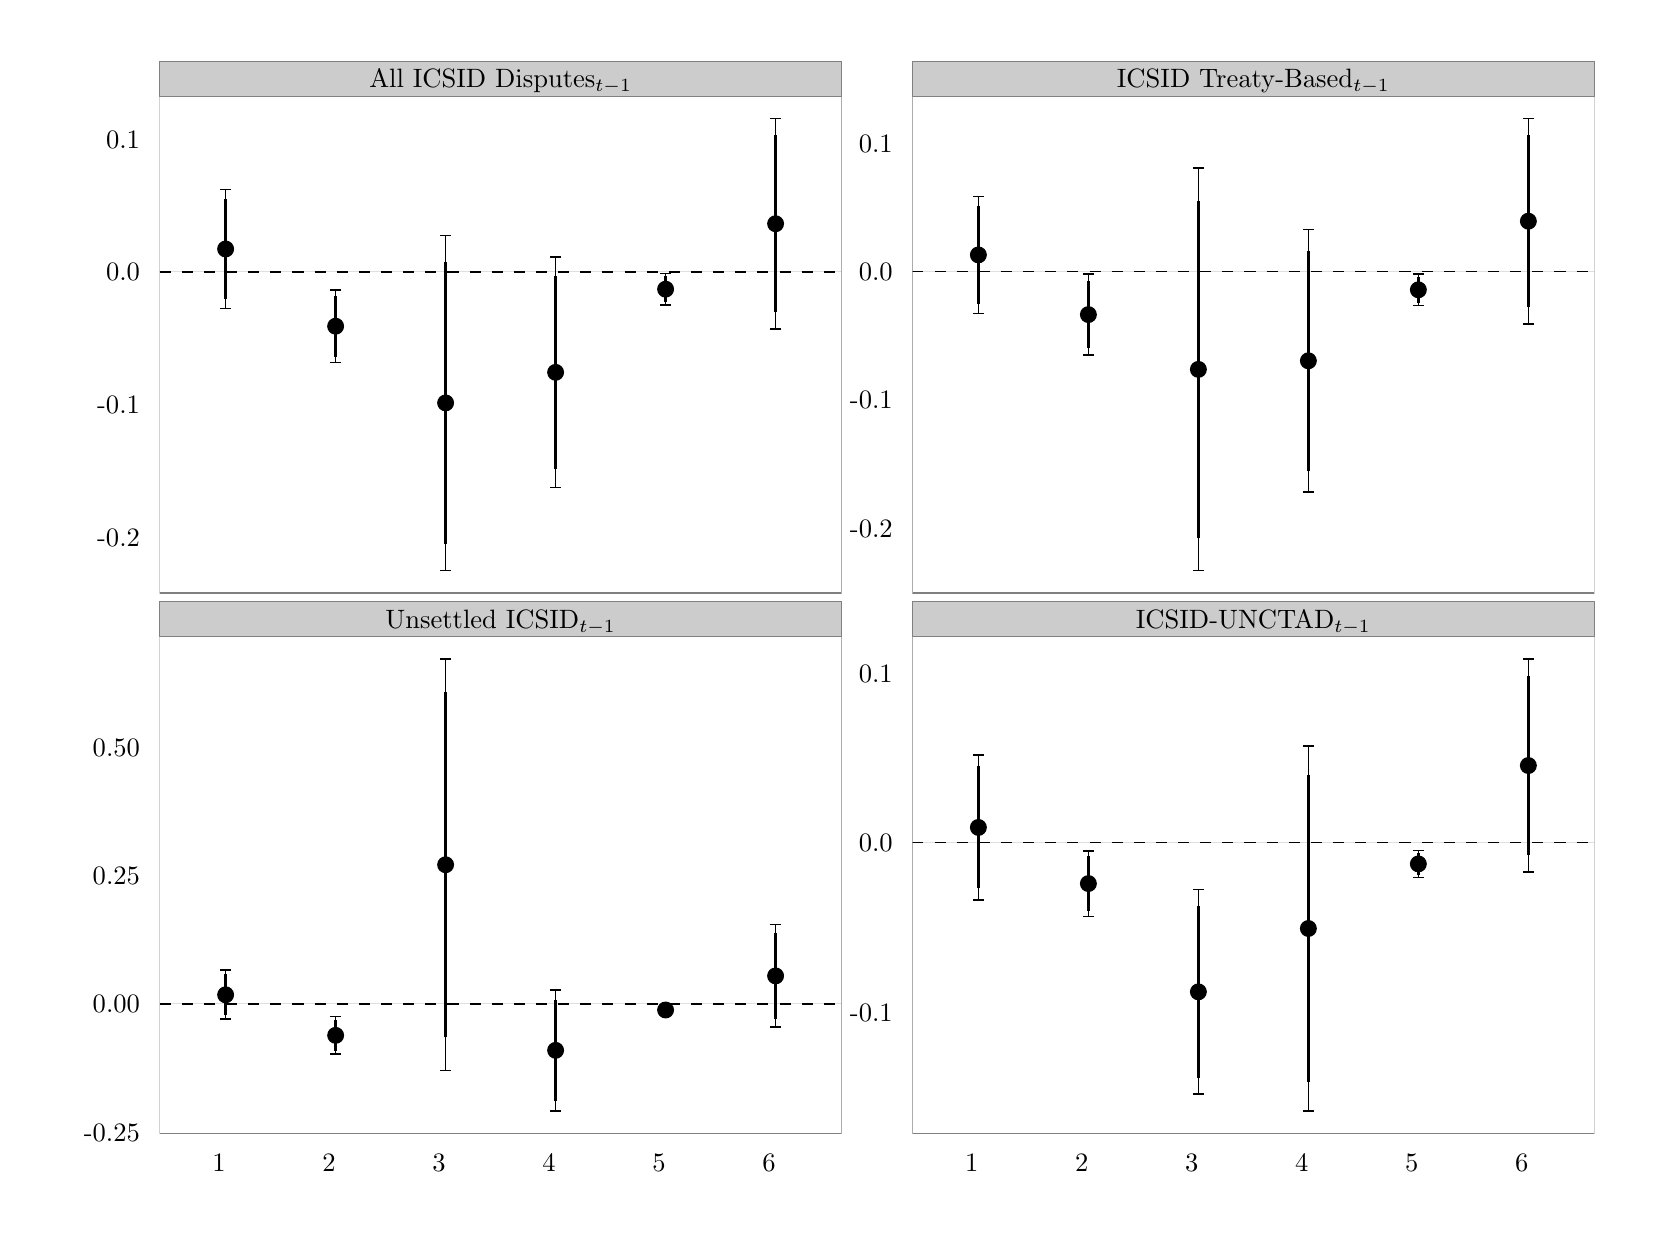
\begin{tikzpicture}[x=1pt,y=1pt]
\definecolor[named]{fillColor}{rgb}{1.00,1.00,1.00}
\path[use as bounding box,fill=fillColor,fill opacity=0.00] (0,0) rectangle (578.16,433.62);
\begin{scope}
\path[clip] (  0.00,  0.00) rectangle (578.16,433.62);
\definecolor[named]{drawColor}{rgb}{1.00,1.00,1.00}
\definecolor[named]{fillColor}{rgb}{1.00,1.00,1.00}

\path[draw=drawColor,line width= 0.6pt,line join=round,line cap=round,fill=fillColor] (  0.00,  0.00) rectangle (578.16,433.62);
\end{scope}
\begin{scope}
\path[clip] ( 47.68,229.31) rectangle (294.11,408.94);
\definecolor[named]{fillColor}{rgb}{1.00,1.00,1.00}

\path[fill=fillColor] ( 47.68,229.31) rectangle (294.11,408.94);
\definecolor[named]{drawColor}{rgb}{0.00,0.00,0.00}
\definecolor[named]{fillColor}{rgb}{0.00,0.00,0.00}

\path[draw=drawColor,draw opacity=0.30,line width= 0.3pt,line join=round,fill=fillColor,fill opacity=0.30] ( 71.53,332.16) -- ( 71.53,375.12);

\path[draw=drawColor,draw opacity=0.30,line width= 0.3pt,line join=round,fill=fillColor,fill opacity=0.30] (111.28,312.60) -- (111.28,338.88);

\path[draw=drawColor,draw opacity=0.30,line width= 0.3pt,line join=round,fill=fillColor,fill opacity=0.30] (151.02,237.48) -- (151.02,358.57);

\path[draw=drawColor,draw opacity=0.30,line width= 0.3pt,line join=round,fill=fillColor,fill opacity=0.30] (190.77,267.44) -- (190.77,350.71);

\path[draw=drawColor,draw opacity=0.30,line width= 0.3pt,line join=round,fill=fillColor,fill opacity=0.30] (230.51,333.46) -- (230.51,344.77);

\path[draw=drawColor,draw opacity=0.30,line width= 0.3pt,line join=round,fill=fillColor,fill opacity=0.30] (270.26,324.76) -- (270.26,400.78);
\definecolor[named]{drawColor}{rgb}{0.00,0.00,0.00}
\definecolor[named]{fillColor}{rgb}{0.00,0.00,0.00}

\path[draw=drawColor,line width= 1.1pt,line join=round,fill=fillColor] ( 71.53,335.62) -- ( 71.53,371.66);

\path[draw=drawColor,line width= 1.1pt,line join=round,fill=fillColor] (111.28,314.71) -- (111.28,336.77);

\path[draw=drawColor,line width= 1.1pt,line join=round,fill=fillColor] (151.02,247.21) -- (151.02,348.84);

\path[draw=drawColor,line width= 1.1pt,line join=round,fill=fillColor] (190.77,274.13) -- (190.77,344.02);

\path[draw=drawColor,line width= 1.1pt,line join=round,fill=fillColor] (230.51,334.37) -- (230.51,343.86);

\path[draw=drawColor,line width= 1.1pt,line join=round,fill=fillColor] (270.26,330.88) -- (270.26,394.67);

\path[draw=drawColor,line width= 0.6pt,dash pattern=on 4pt off 4pt ,line join=round,fill=fillColor] ( 47.68,345.41) -- (294.11,345.41);

\path[draw=drawColor,line width= 0.4pt,line join=round,line cap=round,fill=fillColor] ( 71.53,353.64) circle (  2.85);

\path[draw=drawColor,line width= 0.4pt,line join=round,line cap=round,fill=fillColor] (111.28,325.74) circle (  2.85);

\path[draw=drawColor,line width= 0.4pt,line join=round,line cap=round,fill=fillColor] (151.02,298.02) circle (  2.85);

\path[draw=drawColor,line width= 0.4pt,line join=round,line cap=round,fill=fillColor] (190.77,309.07) circle (  2.85);

\path[draw=drawColor,line width= 0.4pt,line join=round,line cap=round,fill=fillColor] (230.51,339.12) circle (  2.85);

\path[draw=drawColor,line width= 0.4pt,line join=round,line cap=round,fill=fillColor] (270.26,362.77) circle (  2.85);

\path[draw=drawColor,line width= 0.6pt,line join=round] ( 69.54,375.12) --
	( 73.52,375.12);

\path[draw=drawColor,line width= 0.6pt,line join=round] ( 71.53,375.12) --
	( 71.53,332.16);

\path[draw=drawColor,line width= 0.6pt,line join=round] ( 69.54,332.16) --
	( 73.52,332.16);

\path[draw=drawColor,line width= 0.6pt,line join=round] (109.29,338.88) --
	(113.26,338.88);

\path[draw=drawColor,line width= 0.6pt,line join=round] (111.28,338.88) --
	(111.28,312.60);

\path[draw=drawColor,line width= 0.6pt,line join=round] (109.29,312.60) --
	(113.26,312.60);

\path[draw=drawColor,line width= 0.6pt,line join=round] (149.04,358.57) --
	(153.01,358.57);

\path[draw=drawColor,line width= 0.6pt,line join=round] (151.02,358.57) --
	(151.02,237.48);

\path[draw=drawColor,line width= 0.6pt,line join=round] (149.04,237.48) --
	(153.01,237.48);

\path[draw=drawColor,line width= 0.6pt,line join=round] (188.78,350.71) --
	(192.76,350.71);

\path[draw=drawColor,line width= 0.6pt,line join=round] (190.77,350.71) --
	(190.77,267.44);

\path[draw=drawColor,line width= 0.6pt,line join=round] (188.78,267.44) --
	(192.76,267.44);

\path[draw=drawColor,line width= 0.6pt,line join=round] (228.53,344.77) --
	(232.50,344.77);

\path[draw=drawColor,line width= 0.6pt,line join=round] (230.51,344.77) --
	(230.51,333.46);

\path[draw=drawColor,line width= 0.6pt,line join=round] (228.53,333.46) --
	(232.50,333.46);

\path[draw=drawColor,line width= 0.6pt,line join=round] (268.27,400.78) --
	(272.25,400.78);

\path[draw=drawColor,line width= 0.6pt,line join=round] (270.26,400.78) --
	(270.26,324.76);

\path[draw=drawColor,line width= 0.6pt,line join=round] (268.27,324.76) --
	(272.25,324.76);
\definecolor[named]{drawColor}{rgb}{0.50,0.50,0.50}

\path[draw=drawColor,line width= 0.6pt,line join=round,line cap=round] ( 47.68,229.31) rectangle (294.11,408.94);
\end{scope}
\begin{scope}
\path[clip] (319.69,229.31) rectangle (566.12,408.94);
\definecolor[named]{fillColor}{rgb}{1.00,1.00,1.00}

\path[fill=fillColor] (319.69,229.31) rectangle (566.12,408.94);
\definecolor[named]{drawColor}{rgb}{0.00,0.00,0.00}
\definecolor[named]{fillColor}{rgb}{0.00,0.00,0.00}

\path[draw=drawColor,draw opacity=0.30,line width= 0.3pt,line join=round,fill=fillColor,fill opacity=0.30] (343.54,330.36) -- (343.54,372.64);

\path[draw=drawColor,draw opacity=0.30,line width= 0.3pt,line join=round,fill=fillColor,fill opacity=0.30] (383.29,315.38) -- (383.29,344.51);

\path[draw=drawColor,draw opacity=0.30,line width= 0.3pt,line join=round,fill=fillColor,fill opacity=0.30] (423.03,237.48) -- (423.03,382.81);

\path[draw=drawColor,draw opacity=0.30,line width= 0.3pt,line join=round,fill=fillColor,fill opacity=0.30] (462.78,265.78) -- (462.78,360.69);

\path[draw=drawColor,draw opacity=0.30,line width= 0.3pt,line join=round,fill=fillColor,fill opacity=0.30] (502.52,333.17) -- (502.52,344.62);

\path[draw=drawColor,draw opacity=0.30,line width= 0.3pt,line join=round,fill=fillColor,fill opacity=0.30] (542.27,326.60) -- (542.27,400.78);
\definecolor[named]{drawColor}{rgb}{0.00,0.00,0.00}
\definecolor[named]{fillColor}{rgb}{0.00,0.00,0.00}

\path[draw=drawColor,line width= 1.1pt,line join=round,fill=fillColor] (343.54,333.76) -- (343.54,369.24);

\path[draw=drawColor,line width= 1.1pt,line join=round,fill=fillColor] (383.29,317.72) -- (383.29,342.17);

\path[draw=drawColor,line width= 1.1pt,line join=round,fill=fillColor] (423.03,249.16) -- (423.03,371.13);

\path[draw=drawColor,line width= 1.1pt,line join=round,fill=fillColor] (462.78,273.41) -- (462.78,353.06);

\path[draw=drawColor,line width= 1.1pt,line join=round,fill=fillColor] (502.52,334.09) -- (502.52,343.70);

\path[draw=drawColor,line width= 1.1pt,line join=round,fill=fillColor] (542.27,332.57) -- (542.27,394.81);

\path[draw=drawColor,line width= 0.6pt,dash pattern=on 4pt off 4pt ,line join=round,fill=fillColor] (319.69,345.54) -- (566.12,345.54);

\path[draw=drawColor,line width= 0.4pt,line join=round,line cap=round,fill=fillColor] (343.54,351.50) circle (  2.85);

\path[draw=drawColor,line width= 0.4pt,line join=round,line cap=round,fill=fillColor] (383.29,329.94) circle (  2.85);

\path[draw=drawColor,line width= 0.4pt,line join=round,line cap=round,fill=fillColor] (423.03,310.14) circle (  2.85);

\path[draw=drawColor,line width= 0.4pt,line join=round,line cap=round,fill=fillColor] (462.78,313.24) circle (  2.85);

\path[draw=drawColor,line width= 0.4pt,line join=round,line cap=round,fill=fillColor] (502.52,338.89) circle (  2.85);

\path[draw=drawColor,line width= 0.4pt,line join=round,line cap=round,fill=fillColor] (542.27,363.69) circle (  2.85);

\path[draw=drawColor,line width= 0.6pt,line join=round] (341.55,372.64) --
	(345.53,372.64);

\path[draw=drawColor,line width= 0.6pt,line join=round] (343.54,372.64) --
	(343.54,330.36);

\path[draw=drawColor,line width= 0.6pt,line join=round] (341.55,330.36) --
	(345.53,330.36);

\path[draw=drawColor,line width= 0.6pt,line join=round] (381.30,344.51) --
	(385.27,344.51);

\path[draw=drawColor,line width= 0.6pt,line join=round] (383.29,344.51) --
	(383.29,315.38);

\path[draw=drawColor,line width= 0.6pt,line join=round] (381.30,315.38) --
	(385.27,315.38);

\path[draw=drawColor,line width= 0.6pt,line join=round] (421.04,382.81) --
	(425.02,382.81);

\path[draw=drawColor,line width= 0.6pt,line join=round] (423.03,382.81) --
	(423.03,237.48);

\path[draw=drawColor,line width= 0.6pt,line join=round] (421.04,237.48) --
	(425.02,237.48);

\path[draw=drawColor,line width= 0.6pt,line join=round] (460.79,360.69) --
	(464.76,360.69);

\path[draw=drawColor,line width= 0.6pt,line join=round] (462.78,360.69) --
	(462.78,265.78);

\path[draw=drawColor,line width= 0.6pt,line join=round] (460.79,265.78) --
	(464.76,265.78);

\path[draw=drawColor,line width= 0.6pt,line join=round] (500.54,344.62) --
	(504.51,344.62);

\path[draw=drawColor,line width= 0.6pt,line join=round] (502.52,344.62) --
	(502.52,333.17);

\path[draw=drawColor,line width= 0.6pt,line join=round] (500.54,333.17) --
	(504.51,333.17);

\path[draw=drawColor,line width= 0.6pt,line join=round] (540.28,400.78) --
	(544.26,400.78);

\path[draw=drawColor,line width= 0.6pt,line join=round] (542.27,400.78) --
	(542.27,326.60);

\path[draw=drawColor,line width= 0.6pt,line join=round] (540.28,326.60) --
	(544.26,326.60);
\definecolor[named]{drawColor}{rgb}{0.50,0.50,0.50}

\path[draw=drawColor,line width= 0.6pt,line join=round,line cap=round] (319.69,229.31) rectangle (566.12,408.94);
\end{scope}
\begin{scope}
\path[clip] ( 47.68, 34.03) rectangle (294.11,213.66);
\definecolor[named]{fillColor}{rgb}{1.00,1.00,1.00}

\path[fill=fillColor] ( 47.68, 34.03) rectangle (294.11,213.66);
\definecolor[named]{drawColor}{rgb}{0.00,0.00,0.00}
\definecolor[named]{fillColor}{rgb}{0.00,0.00,0.00}

\path[draw=drawColor,draw opacity=0.30,line width= 0.3pt,line join=round,fill=fillColor,fill opacity=0.30] ( 71.53, 75.31) -- ( 71.53, 92.99);

\path[draw=drawColor,draw opacity=0.30,line width= 0.3pt,line join=round,fill=fillColor,fill opacity=0.30] (111.28, 62.73) -- (111.28, 76.25);

\path[draw=drawColor,draw opacity=0.30,line width= 0.3pt,line join=round,fill=fillColor,fill opacity=0.30] (151.02, 56.77) -- (151.02,205.50);

\path[draw=drawColor,draw opacity=0.30,line width= 0.3pt,line join=round,fill=fillColor,fill opacity=0.30] (190.77, 42.20) -- (190.77, 85.95);

\path[draw=drawColor,draw opacity=0.30,line width= 0.3pt,line join=round,fill=fillColor,fill opacity=0.30] (230.51, 76.74) -- (230.51, 80.57);

\path[draw=drawColor,draw opacity=0.30,line width= 0.3pt,line join=round,fill=fillColor,fill opacity=0.30] (270.26, 72.47) -- (270.26,109.49);
\definecolor[named]{drawColor}{rgb}{0.00,0.00,0.00}
\definecolor[named]{fillColor}{rgb}{0.00,0.00,0.00}

\path[draw=drawColor,line width= 1.1pt,line join=round,fill=fillColor] ( 71.53, 76.74) -- ( 71.53, 91.57);

\path[draw=drawColor,line width= 1.1pt,line join=round,fill=fillColor] (111.28, 63.81) -- (111.28, 75.16);

\path[draw=drawColor,line width= 1.1pt,line join=round,fill=fillColor] (151.02, 68.73) -- (151.02,193.54);

\path[draw=drawColor,line width= 1.1pt,line join=round,fill=fillColor] (190.77, 45.72) -- (190.77, 82.43);

\path[draw=drawColor,line width= 1.1pt,line join=round,fill=fillColor] (230.51, 77.05) -- (230.51, 80.27);

\path[draw=drawColor,line width= 1.1pt,line join=round,fill=fillColor] (270.26, 75.45) -- (270.26,106.52);

\path[draw=drawColor,line width= 0.6pt,dash pattern=on 4pt off 4pt ,line join=round,fill=fillColor] ( 47.68, 80.90) -- (294.11, 80.90);

\path[draw=drawColor,line width= 0.4pt,line join=round,line cap=round,fill=fillColor] ( 71.53, 84.15) circle (  2.85);

\path[draw=drawColor,line width= 0.4pt,line join=round,line cap=round,fill=fillColor] (111.28, 69.49) circle (  2.85);

\path[draw=drawColor,line width= 0.4pt,line join=round,line cap=round,fill=fillColor] (151.02,131.14) circle (  2.85);

\path[draw=drawColor,line width= 0.4pt,line join=round,line cap=round,fill=fillColor] (190.77, 64.08) circle (  2.85);

\path[draw=drawColor,line width= 0.4pt,line join=round,line cap=round,fill=fillColor] (230.51, 78.66) circle (  2.85);

\path[draw=drawColor,line width= 0.4pt,line join=round,line cap=round,fill=fillColor] (270.26, 90.98) circle (  2.85);

\path[draw=drawColor,line width= 0.6pt,line join=round] ( 69.54, 92.99) --
	( 73.52, 92.99);

\path[draw=drawColor,line width= 0.6pt,line join=round] ( 71.53, 92.99) --
	( 71.53, 75.31);

\path[draw=drawColor,line width= 0.6pt,line join=round] ( 69.54, 75.31) --
	( 73.52, 75.31);

\path[draw=drawColor,line width= 0.6pt,line join=round] (109.29, 76.25) --
	(113.26, 76.25);

\path[draw=drawColor,line width= 0.6pt,line join=round] (111.28, 76.25) --
	(111.28, 62.73);

\path[draw=drawColor,line width= 0.6pt,line join=round] (109.29, 62.73) --
	(113.26, 62.73);

\path[draw=drawColor,line width= 0.6pt,line join=round] (149.04,205.50) --
	(153.01,205.50);

\path[draw=drawColor,line width= 0.6pt,line join=round] (151.02,205.50) --
	(151.02, 56.77);

\path[draw=drawColor,line width= 0.6pt,line join=round] (149.04, 56.77) --
	(153.01, 56.77);

\path[draw=drawColor,line width= 0.6pt,line join=round] (188.78, 85.95) --
	(192.76, 85.95);

\path[draw=drawColor,line width= 0.6pt,line join=round] (190.77, 85.95) --
	(190.77, 42.20);

\path[draw=drawColor,line width= 0.6pt,line join=round] (188.78, 42.20) --
	(192.76, 42.20);

\path[draw=drawColor,line width= 0.6pt,line join=round] (228.53, 80.57) --
	(232.50, 80.57);

\path[draw=drawColor,line width= 0.6pt,line join=round] (230.51, 80.57) --
	(230.51, 76.74);

\path[draw=drawColor,line width= 0.6pt,line join=round] (228.53, 76.74) --
	(232.50, 76.74);

\path[draw=drawColor,line width= 0.6pt,line join=round] (268.27,109.49) --
	(272.25,109.49);

\path[draw=drawColor,line width= 0.6pt,line join=round] (270.26,109.49) --
	(270.26, 72.47);

\path[draw=drawColor,line width= 0.6pt,line join=round] (268.27, 72.47) --
	(272.25, 72.47);
\definecolor[named]{drawColor}{rgb}{0.50,0.50,0.50}

\path[draw=drawColor,line width= 0.6pt,line join=round,line cap=round] ( 47.68, 34.03) rectangle (294.11,213.66);
\end{scope}
\begin{scope}
\path[clip] (319.69, 34.03) rectangle (566.12,213.66);
\definecolor[named]{fillColor}{rgb}{1.00,1.00,1.00}

\path[fill=fillColor] (319.69, 34.03) rectangle (566.12,213.66);
\definecolor[named]{drawColor}{rgb}{0.00,0.00,0.00}
\definecolor[named]{fillColor}{rgb}{0.00,0.00,0.00}

\path[draw=drawColor,draw opacity=0.30,line width= 0.3pt,line join=round,fill=fillColor,fill opacity=0.30] (343.54,118.34) -- (343.54,170.90);

\path[draw=drawColor,draw opacity=0.30,line width= 0.3pt,line join=round,fill=fillColor,fill opacity=0.30] (383.29,112.50) -- (383.29,136.17);

\path[draw=drawColor,draw opacity=0.30,line width= 0.3pt,line join=round,fill=fillColor,fill opacity=0.30] (423.03, 48.22) -- (423.03,122.22);

\path[draw=drawColor,draw opacity=0.30,line width= 0.3pt,line join=round,fill=fillColor,fill opacity=0.30] (462.78, 42.20) -- (462.78,174.02);

\path[draw=drawColor,draw opacity=0.30,line width= 0.3pt,line join=round,fill=fillColor,fill opacity=0.30] (502.52,126.53) -- (502.52,136.34);

\path[draw=drawColor,draw opacity=0.30,line width= 0.3pt,line join=round,fill=fillColor,fill opacity=0.30] (542.27,128.48) -- (542.27,205.50);
\definecolor[named]{drawColor}{rgb}{0.00,0.00,0.00}
\definecolor[named]{fillColor}{rgb}{0.00,0.00,0.00}

\path[draw=drawColor,line width= 1.1pt,line join=round,fill=fillColor] (343.54,122.57) -- (343.54,166.67);

\path[draw=drawColor,line width= 1.1pt,line join=round,fill=fillColor] (383.29,114.40) -- (383.29,134.27);

\path[draw=drawColor,line width= 1.1pt,line join=round,fill=fillColor] (423.03, 54.17) -- (423.03,116.27);

\path[draw=drawColor,line width= 1.1pt,line join=round,fill=fillColor] (462.78, 52.80) -- (462.78,163.42);

\path[draw=drawColor,line width= 1.1pt,line join=round,fill=fillColor] (502.52,127.32) -- (502.52,135.55);

\path[draw=drawColor,line width= 1.1pt,line join=round,fill=fillColor] (542.27,134.67) -- (542.27,199.31);

\path[draw=drawColor,line width= 0.6pt,dash pattern=on 4pt off 4pt ,line join=round,fill=fillColor] (319.69,139.13) -- (566.12,139.13);

\path[draw=drawColor,line width= 0.4pt,line join=round,line cap=round,fill=fillColor] (343.54,144.62) circle (  2.85);

\path[draw=drawColor,line width= 0.4pt,line join=round,line cap=round,fill=fillColor] (383.29,124.34) circle (  2.85);

\path[draw=drawColor,line width= 0.4pt,line join=round,line cap=round,fill=fillColor] (423.03, 85.22) circle (  2.85);

\path[draw=drawColor,line width= 0.4pt,line join=round,line cap=round,fill=fillColor] (462.78,108.11) circle (  2.85);

\path[draw=drawColor,line width= 0.4pt,line join=round,line cap=round,fill=fillColor] (502.52,131.44) circle (  2.85);

\path[draw=drawColor,line width= 0.4pt,line join=round,line cap=round,fill=fillColor] (542.27,166.99) circle (  2.85);

\path[draw=drawColor,line width= 0.6pt,line join=round] (341.55,170.90) --
	(345.53,170.90);

\path[draw=drawColor,line width= 0.6pt,line join=round] (343.54,170.90) --
	(343.54,118.34);

\path[draw=drawColor,line width= 0.6pt,line join=round] (341.55,118.34) --
	(345.53,118.34);

\path[draw=drawColor,line width= 0.6pt,line join=round] (381.30,136.17) --
	(385.27,136.17);

\path[draw=drawColor,line width= 0.6pt,line join=round] (383.29,136.17) --
	(383.29,112.50);

\path[draw=drawColor,line width= 0.6pt,line join=round] (381.30,112.50) --
	(385.27,112.50);

\path[draw=drawColor,line width= 0.6pt,line join=round] (421.04,122.22) --
	(425.02,122.22);

\path[draw=drawColor,line width= 0.6pt,line join=round] (423.03,122.22) --
	(423.03, 48.22);

\path[draw=drawColor,line width= 0.6pt,line join=round] (421.04, 48.22) --
	(425.02, 48.22);

\path[draw=drawColor,line width= 0.6pt,line join=round] (460.79,174.02) --
	(464.76,174.02);

\path[draw=drawColor,line width= 0.6pt,line join=round] (462.78,174.02) --
	(462.78, 42.20);

\path[draw=drawColor,line width= 0.6pt,line join=round] (460.79, 42.20) --
	(464.76, 42.20);

\path[draw=drawColor,line width= 0.6pt,line join=round] (500.54,136.34) --
	(504.51,136.34);

\path[draw=drawColor,line width= 0.6pt,line join=round] (502.52,136.34) --
	(502.52,126.53);

\path[draw=drawColor,line width= 0.6pt,line join=round] (500.54,126.53) --
	(504.51,126.53);

\path[draw=drawColor,line width= 0.6pt,line join=round] (540.28,205.50) --
	(544.26,205.50);

\path[draw=drawColor,line width= 0.6pt,line join=round] (542.27,205.50) --
	(542.27,128.48);

\path[draw=drawColor,line width= 0.6pt,line join=round] (540.28,128.48) --
	(544.26,128.48);
\definecolor[named]{drawColor}{rgb}{0.50,0.50,0.50}

\path[draw=drawColor,line width= 0.6pt,line join=round,line cap=round] (319.69, 34.03) rectangle (566.12,213.66);
\end{scope}
\begin{scope}
\path[clip] (  0.00,  0.00) rectangle (578.16,433.62);
\definecolor[named]{drawColor}{rgb}{0.50,0.50,0.50}
\definecolor[named]{fillColor}{rgb}{0.80,0.80,0.80}

\path[draw=drawColor,line width= 0.2pt,line join=round,line cap=round,fill=fillColor] ( 47.68,408.94) rectangle (294.11,421.57);
\definecolor[named]{drawColor}{rgb}{0.00,0.00,0.00}

\node[text=drawColor,anchor=base,inner sep=0pt, outer sep=0pt, scale=  0.96] at (170.90,411.95) {All ICSID Disputes$_{t-1}$};
\end{scope}
\begin{scope}
\path[clip] (  0.00,  0.00) rectangle (578.16,433.62);
\definecolor[named]{drawColor}{rgb}{0.50,0.50,0.50}
\definecolor[named]{fillColor}{rgb}{0.80,0.80,0.80}

\path[draw=drawColor,line width= 0.2pt,line join=round,line cap=round,fill=fillColor] (319.69,408.94) rectangle (566.12,421.57);
\definecolor[named]{drawColor}{rgb}{0.00,0.00,0.00}

\node[text=drawColor,anchor=base,inner sep=0pt, outer sep=0pt, scale=  0.96] at (442.90,411.95) {ICSID Treaty-Based$_{t-1}$};
\end{scope}
\begin{scope}
\path[clip] (  0.00,  0.00) rectangle (578.16,433.62);
\definecolor[named]{drawColor}{rgb}{0.50,0.50,0.50}
\definecolor[named]{fillColor}{rgb}{0.80,0.80,0.80}

\path[draw=drawColor,line width= 0.2pt,line join=round,line cap=round,fill=fillColor] ( 47.68,213.66) rectangle (294.11,226.30);
\definecolor[named]{drawColor}{rgb}{0.00,0.00,0.00}

\node[text=drawColor,anchor=base,inner sep=0pt, outer sep=0pt, scale=  0.96] at (170.90,216.68) {Unsettled ICSID$_{t-1}$};
\end{scope}
\begin{scope}
\path[clip] (  0.00,  0.00) rectangle (578.16,433.62);
\definecolor[named]{drawColor}{rgb}{0.50,0.50,0.50}
\definecolor[named]{fillColor}{rgb}{0.80,0.80,0.80}

\path[draw=drawColor,line width= 0.2pt,line join=round,line cap=round,fill=fillColor] (319.69,213.66) rectangle (566.12,226.30);
\definecolor[named]{drawColor}{rgb}{0.00,0.00,0.00}

\node[text=drawColor,anchor=base,inner sep=0pt, outer sep=0pt, scale=  0.96] at (442.90,216.68) {ICSID-UNCTAD$_{t-1}$};
\end{scope}
\begin{scope}
\path[clip] (  0.00,  0.00) rectangle (578.16,433.62);
\definecolor[named]{drawColor}{rgb}{0.00,0.00,0.00}

\node[text=drawColor,anchor=base east,inner sep=0pt, outer sep=0pt, scale=  0.96] at ( 40.57,246.13) {-0.2};

\node[text=drawColor,anchor=base east,inner sep=0pt, outer sep=0pt, scale=  0.96] at ( 40.57,294.12) {-0.1};

\node[text=drawColor,anchor=base east,inner sep=0pt, outer sep=0pt, scale=  0.96] at ( 40.57,342.11) {0.0};

\node[text=drawColor,anchor=base east,inner sep=0pt, outer sep=0pt, scale=  0.96] at ( 40.57,390.09) {0.1};
\end{scope}
\begin{scope}
\path[clip] (  0.00,  0.00) rectangle (578.16,433.62);
\definecolor[named]{drawColor}{rgb}{0.00,0.00,0.00}

\node[text=drawColor,anchor=base east,inner sep=0pt, outer sep=0pt, scale=  0.96] at (312.58,249.43) {-0.2};

\node[text=drawColor,anchor=base east,inner sep=0pt, outer sep=0pt, scale=  0.96] at (312.58,295.83) {-0.1};

\node[text=drawColor,anchor=base east,inner sep=0pt, outer sep=0pt, scale=  0.96] at (312.58,342.24) {0.0};

\node[text=drawColor,anchor=base east,inner sep=0pt, outer sep=0pt, scale=  0.96] at (312.58,388.64) {0.1};
\end{scope}
\begin{scope}
\path[clip] (  0.00,  0.00) rectangle (578.16,433.62);
\definecolor[named]{drawColor}{rgb}{0.00,0.00,0.00}

\node[text=drawColor,anchor=base east,inner sep=0pt, outer sep=0pt, scale=  0.96] at ( 40.57, 31.23) {-0.25};

\node[text=drawColor,anchor=base east,inner sep=0pt, outer sep=0pt, scale=  0.96] at ( 40.57, 77.59) {0.00};

\node[text=drawColor,anchor=base east,inner sep=0pt, outer sep=0pt, scale=  0.96] at ( 40.57,123.96) {0.25};

\node[text=drawColor,anchor=base east,inner sep=0pt, outer sep=0pt, scale=  0.96] at ( 40.57,170.32) {0.50};
\end{scope}
\begin{scope}
\path[clip] (  0.00,  0.00) rectangle (578.16,433.62);
\definecolor[named]{drawColor}{rgb}{0.00,0.00,0.00}

\node[text=drawColor,anchor=base east,inner sep=0pt, outer sep=0pt, scale=  0.96] at (312.58, 74.49) {-0.1};

\node[text=drawColor,anchor=base east,inner sep=0pt, outer sep=0pt, scale=  0.96] at (312.58,135.83) {0.0};

\node[text=drawColor,anchor=base east,inner sep=0pt, outer sep=0pt, scale=  0.96] at (312.58,197.17) {0.1};
\end{scope}
\begin{scope}
\path[clip] (  0.00,  0.00) rectangle (578.16,433.62);
\definecolor[named]{drawColor}{rgb}{0.00,0.00,0.00}

\node[text=drawColor,anchor=base east,inner sep=0pt, outer sep=0pt, scale=  0.96] at ( 71.53, 20.31) {1};

\node[text=drawColor,anchor=base east,inner sep=0pt, outer sep=0pt, scale=  0.96] at (111.28, 20.31) {2};

\node[text=drawColor,anchor=base east,inner sep=0pt, outer sep=0pt, scale=  0.96] at (151.02, 20.31) {3};

\node[text=drawColor,anchor=base east,inner sep=0pt, outer sep=0pt, scale=  0.96] at (190.77, 20.31) {4};

\node[text=drawColor,anchor=base east,inner sep=0pt, outer sep=0pt, scale=  0.96] at (230.51, 20.31) {5};

\node[text=drawColor,anchor=base east,inner sep=0pt, outer sep=0pt, scale=  0.96] at (270.26, 20.31) {6};
\end{scope}
\begin{scope}
\path[clip] (  0.00,  0.00) rectangle (578.16,433.62);
\definecolor[named]{drawColor}{rgb}{0.00,0.00,0.00}

\node[text=drawColor,anchor=base east,inner sep=0pt, outer sep=0pt, scale=  0.96] at (343.54, 20.31) {1};

\node[text=drawColor,anchor=base east,inner sep=0pt, outer sep=0pt, scale=  0.96] at (383.29, 20.31) {2};

\node[text=drawColor,anchor=base east,inner sep=0pt, outer sep=0pt, scale=  0.96] at (423.03, 20.31) {3};

\node[text=drawColor,anchor=base east,inner sep=0pt, outer sep=0pt, scale=  0.96] at (462.78, 20.31) {4};

\node[text=drawColor,anchor=base east,inner sep=0pt, outer sep=0pt, scale=  0.96] at (502.52, 20.31) {5};

\node[text=drawColor,anchor=base east,inner sep=0pt, outer sep=0pt, scale=  0.96] at (542.27, 20.31) {6};
\end{scope}
\end{tikzpicture}
}	
	\caption*{Note: Each line here shows the coefficient estimate of one of the lagged dispute variables from rerunning the model on a random subsample within the dataset. All the covariates used in the initial model shown in table \ref{tab:ecm} were included as well.}
\end{figure}

The findings with respect to other independent variables in the model are largely consistent with those reported above in Table \ref{tab:dispRepLevel}, but weaker. Again the coefficients for the lagged population, internal stability and ratified BITs are statistically significant in the anticipated direction, as are the coefficients for changes in capital openness, GDP, and population. Changes in the rate of inflation also have an impact on reputation, but only with respect to the estimates for the UNCTAD dispute data. In addition, the strength of the coefficient of lagged reputation in the ECM model underlines the tendency for investment profile ratings to remain relatively stable over time.

\section*{Conclusion}

This paper contributes to the growing body of literature on international investor-state disputes by clarifying their consequences. Whereas prior research has claimed that alleged treaty violations are predictably translated into reduced foreign direct investment flows, we find no evidence of such an effect. We therefore turn to the analysis of reputational damage, which is the mechanism presumed to be brought into play by perceptions that a state has failed to live up to its treaty violations. Consistent with the literature on international commitments, we find evidence that states incur reputational costs for having arbitral claims filed against them, regardless of the venue or outcome of the ISDS process. On the other hand, the substantive significance of these findings is limited. Relative to country fundamentals, such as economic dynamism, size, or internal stability, investor-state disputes, including those brought under international treaties, have a modest impact on reputation. As emphasized by our ECM analysis, reputational costs only emerge slowly over time as a country accumulates a record of repeated dispute involvement. Individual disputes, whether treaty-based or not, have no immediate  impact on investment reputation. Thus whereas the logic underlying the credible commitment story espoused in the BITs literature assumes that states incur significant reputational costs from alleged violations of international agreements, we show that the effects of involvement in investor-state disputes are circumscribed with respect to investment reputation and completely inconsequential with respect to FDI flows.

These findings have significant implications for the broader body of literature on international institutions. Existing theory assumes that formal international commitments raise the ex post cost of defection, thereby creating incentives for states to comply with their treaty obligations. Our analysis significantly modifies this expectation by suggesting that the strength of the incentives for compliance is likely to vary with the breadth, visibility, and legitimacy of the monitoring, sanctioning, and enforcement mechanisms brought into play by particular sets of international institutions. Under the current ISDS regime, the monitoring of treaty compliance is externalized to individual private firms and ad hoc arbitral tribunals, whose deliberations are limited to the facts of a particular case, unpredictable, less than transparent, prolonged, and potentially reversible. Other characteristics of the ISDS regime further reduce its effectiveness, including the contested legitimacy of international arbitral processes,  related concerns about the independence, impartiality, and lack of restraint of arbitral panels, and  tensions between the treaty protections accorded investors and other sets of international norms. Notwithstanding the legal powers enjoyed by investors under international treaty agreements, the reputational risks of state involvement in ISDS processes are accordingly significantly attenuated. 

\newpage

\bibliographystyle{APSR}
\bibliography{dispRepRefs}

% Insert in tables and figures

\processdelayedfloats 

\newpage

\section*{Appendix}
\label{appendix}

\appendix
\setcounter{figure}{0} \renewcommand{\thefigure}{A.\arabic{figure}}
\setcounter{table}{0} \renewcommand{\thetable}{A.\arabic{table}}

\begin{table}[ht]
\centering
\caption{Descriptive Statistics}
\label{tab:descStats}
\begin{tabular}{lcccccc}
	  \hline\hline
	  & N & n & Mean & Std. Dev. & Min & Max \\ 
	  \hline
Investment Profile & 112 & 2658 & 6.94 & 2.42 & 0.00 & 12.00 \\ 
  All ICSID Disputes (Two Year Sum) & 112 & 2644 & 0.21 & 0.94 & 0.00 & 25.00 \\ 
  ICSID Treaty-Based (Two Year Sum) & 112 & 2644 & 0.18 & 0.92 & 0.00 & 25.00 \\ 
  Unsettled ICSID (Two Year Sum) & 112 & 2644 & 0.13 & 0.69 & 0.00 & 15.00 \\ 
  ICSID-UNCTAD (Two Year Sum) & 112 & 2644 & 0.24 & 1.09 & 0.00 & 29.00 \\ 
  \%$\Delta$ GDP & 109 & 2511 & 0.09 & 0.17 & -0.80 & 1.43 \\ 
  Ln(Pop.) & 111 & 2627 & 16.12 & 1.60 & 12.35 & 21.02 \\ 
  Ln(Inflation) & 108 & 2355 & 3.31 & 0.71 & -4.61 & 10.10 \\ 
  Internal Stability & 112 & 2658 & 8.48 & 2.46 & 0.00 & 12.00 \\ 
  Ratif. BITs & 111 & 2633 & 12.20 & 15.14 & 0.00 & 101.00 \\ 
  Capital Openness & 107 & 2469 & -0.02 & 1.53 & -1.86 & 2.44 \\ 
  Polity & 109 & 2583 & 11.01 & 7.09 & 0.00 & 20.00 \\ 
	   \hline\hline
\end{tabular}
\end{table}

% \newpage

% latex table generated in R 3.0.2 by xtable 1.7-3 package
% Mon May 19 17:07:53 2014
\begin{table}[ht]
\centering
\caption{Investor-State Disputes and International Investment Risk Profile (Using Semi-Balanced Panel, $T \; \geq 17 \;  \forall$ countries)}
\label{tab:dispRepLevelBal}
\begin{tabular}{lr@{} lr@{}lr@{}lr@{}lr@{}}
  \hline\hline
  & \multicolumn{2}{c}{All ICSID} & \multicolumn{2}{c}{ICSID} & \multicolumn{2}{c}{Unsettled$^{a}$} & \multicolumn{2}{c}{ICSID-} \\ 
  & \multicolumn{2}{c}{Disputes} & \multicolumn{2}{c}{Treaty-Based} & \multicolumn{2}{c}{ICSID} & \multicolumn{2}{c}{UNCTAD} \\
 \hline
Registered Disputes$_{(t-1) + (t-2)}$ & $-0$&$.151^{\ast}$ & $-0$&$.162^{\ast}$ & $-0$&$.218^{\ast}$ & -0&.122 \\ 
   & (0&.067) & (0&.076) & (0&.091) & (0&.063) \\ 
  \%$\Delta$ GDP$_{t-1}$ & $0$&$.543^{\ast}$ & $0$&$.543^{\ast}$ & $0$&$.538^{\ast}$ & $0$&$.541^{\ast}$ \\ 
   & (0&.246) & (0&.246) & (0&.245) & (0&.247) \\ 
  Ln(Pop.)$_{t-1}$ & $3$&$.573^{\ast\ast}$ & $3$&$.559^{\ast\ast}$ & $3$&$.545^{\ast\ast}$ & $3$&$.553^{\ast\ast}$ \\ 
   & (0&.602) & (0&.603) & (0&.605) & (0&.605) \\ 
  Ln(Inflation)$_{t-1}$ & $-0$&$.388^{\ast\ast}$ & $-0$&$.388^{\ast\ast}$ & $-0$&$.384^{\ast\ast}$ & $-0$&$.386^{\ast\ast}$ \\ 
   & (0&.112) & (0&.112) & (0&.111) & (0&.113) \\ 
  Internal Stability$_{t-1}$ & $0$&$.183^{\ast\ast}$ & $0$&$.182^{\ast\ast}$ & $0$&$.183^{\ast\ast}$ & $0$&$.183^{\ast\ast}$ \\ 
   & (0&.033) & (0&.033) & (0&.034) & (0&.033) \\ 
  Ratif. BITs$_{t-1}$ & $0$&$.035^{\ast\ast}$ & $0$&$.035^{\ast\ast}$ & $0$&$.035^{\ast\ast}$ & $0$&$.035^{\ast\ast}$ \\ 
   & (0&.011) & (0&.011) & (0&.01) & (0&.011) \\ 
  Capital Openness$_{t-1}$ & $0$&$.202^{\ast}$ & $0$&$.201^{\ast}$ & $0$&$.202^{\ast}$ & $0$&$.2^{\ast}$ \\ 
   & (0&.088) & (0&.088) & (0&.088) & (0&.088) \\ 
  Polity$_{t-1}$ & $0$&$.034^{\ast}$ & $0$&$.034^{\ast}$ & $0$&$.035^{\ast}$ & $0$&$.034^{\ast}$ \\ 
   & (0&.016) & (0&.016) & (0&.016) & (0&.016) \\ 
   \hline
n & 1&884 & 1&884 & 1&884 & 1&884 \\ 
  N && 79 && 79 && 79 && 79 \\ 
  $R^{2}$ & 0&.45 & 0&.45 & 0&.45 & 0&.45 \\ 
  Adj. $R^{2}$ & 0&.43 & 0&.43 & 0&.43 & 0&.43 \\ 
  RMSE & 1&.32 & 1&.32 & 1&.32 & 1&.32 \\ 
   \hline
\hline
\end{tabular}
\caption*{Note: Fixed-effects estimation with standard errors clustered on country using a balanced panel. Standard errors in parentheses. $^{**}$ and $^{*}$ indicate significance at $p<0.01$ and $p<0.05$, respectively. \\ a: The ``unsettled'' category excludes treaty disputes that were resolved via settlement or discontinuation prior to ICSID arbitration.}
\end{table}

\newpage

%\newpage
%About the authors: \\

\end{document}
\bye